%%%%%%%% ICML 2020 EXAMPLE LATEX SUBMISSION FILE %%%%%%%%%%%%%%%%%

\documentclass{article}

% Recommended, but optional, packages for figures and better typesetting:
% \usepackage{subfigure}

\usepackage{booktabs}       % professional-quality tables
\usepackage{amsfonts}       % blackboard math symbols
\usepackage{nicefrac}       % compact symbols for 1/2, etc.
\usepackage{microtype}      % microtypography
\usepackage{graphicx}
\usepackage{multirow}
\usepackage{amsmath}
\usepackage{amssymb}
\usepackage{subcaption}
\usepackage{paralist}
\usepackage{tabularx}
\usepackage{xcolor}
\usepackage[noend]{algpseudocode}
\usepackage{setspace}
\usepackage{enumitem}
\usepackage{subcaption}
% operators

\newcommand{\argmax}{\operatornamewithlimits{argmax}}
\newcommand{\argmin}{\operatornamewithlimits{argmin}}

% vectors
\let\avec\vec
%\renewcommand{\vec}[1]{\ensuremath{\boldsymbol{#1}}}
\renewcommand{\v}[1]{\ensuremath{\boldsymbol{#1}}}

\newcommand{\src}{\lstinline[mathescape, keepspaces]}
\newcommand{\msrc}[1]{\mbox{\src!#1!}}

\newcommand{\tens}[1]{%
  \mathbin{\mathop{\otimes}\limits_{#1}}%
}

% symbol shorthands (lowercase)
%\newcommand{\x}{\ensuremath{\v{x}}}
%\newcommand{\y}{\ensuremath{\v{y}}}
%\newcommand{\z}{\ensuremath{\v{z}}}
%\newcommand{\h}{\v{\eta}}
%\newcommand{\e}{\v{\epsilon}}
%\renewcommand{\u}{\v{u}}
\newcommand{\pd}{\ensuremath{\partial}}
\newcommand{\x}{\ensuremath{x}}
\newcommand{\y}{\ensuremath{y}}
\newcommand{\z}{\ensuremath{z}}
\newcommand{\h}{\ensuremath{\eta}}
\newcommand{\e}{\ensuremath{\epsilon}}
\renewcommand{\u}{\ensuremath{u}}
\newcommand{\q}{\theta}
\newcommand{\f}{\phi}
\renewcommand{\l}{\lambda}
\renewcommand{\t}{\tau}

% symbol shorthands (uppercase)
\renewcommand{\L}{\ensuremath{\mathcal{L}}}
\newcommand{\KL}[2]{\ensuremath{\mathrm{KL}\left({#1} \:\middle\vert\middle\vert\: {#2}\right)}}
\newcommand{\E}{\ensuremath{\mathbb{E}}}
\newcommand{\N}{\ensuremath{\mathcal{N}}}
\newcommand{\C}{\ensuremath{\mathtt{Concrete}}}

%\let\lmid\mid
%\renewcommand{\mid}{\!\lmid\!}

\newcommand{\eval}{\ensuremath{$\reflectbox{$\,\leadsto\,$}$}}
%\newcommand{\eval}{\sim}
\newcommand{\hide}[1]{}

\makeatletter
\DeclareRobustCommand{\cev}[1]{%
  \mathpalette\do@cev{#1}%
}
\newcommand{\do@cev}[2]{%
  \fix@cev{#1}{+}%
  \reflectbox{$\m@th#1\vec{\reflectbox{$\fix@cev{#1}{-}\m@th#1#2\fix@cev{#1}{+}$}}$}%
  \fix@cev{#1}{-}%
}
\newcommand{\fix@cev}[2]{%
  \ifx#1\displaystyle
    \mkern#23mu
  \else
    \ifx#1\textstyle
      \mkern#23mu
    \else
      \ifx#1\scriptstyle
        \mkern#22mu
      \else
        \mkern#22mu
      \fi
    \fi
  \fi
}


\definecolor[named]{Blue}{cmyk}{1,0.1,0,0.1}
\definecolor[named]{Yellow}{cmyk}{0,0.16,1,0}
\definecolor[named]{Orange}{cmyk}{0,0.42,1,0.01}
\definecolor[named]{Red}{cmyk}{0,0.90,0.86,0}
\definecolor[named]{LightBlue}{cmyk}{0.49,0.01,0,0}
\definecolor[named]{Green}{cmyk}{0.20,0,1,0.19}
\definecolor[named]{Purple}{cmyk}{0.55,1,0,0.15}
\definecolor[named]{DarkBlue}{cmyk}{1,0.58,0,0.21}

\usepackage[acronym,smallcaps,nowarn,section,nogroupskip,nonumberlist]{glossaries}
\glsdisablehyper{}
\newacronym{SCFM}{scfm}{stochastic control-flow model}
\newacronym{WS}{ws}{wake-sleep}
\newacronym{BWS}{bws}{basic wake-sleep}
\newacronym{RWS}{rws}{reweighted wake-sleep}
\newacronym{ELBO}{elbo}{evidence lower bound}
\newacronym{VAE}{vae}{variational autoencoder}
\newacronym{IWAE}{iwae}{importance weighted autoencoder}
\newacronym{KL}{kl}{Kullback-Leibler}
\newacronym{SGD}{sgd}{stochastic gradient descent}
\newacronym{VIMCO}{vimco}{variational inference for Monte Carlo objectives}
\newacronym{WW}{ww}{wake-wake}
\newacronym{WWS}{wws}{wake-wake-sleep}
\newacronym{AIR}{air}{Attend, Infer, Repeat}
\newacronym{ESS}{ess}{effective sample size}
\newacronym{REINFORCE}{reinforce}{Reinforce gradient estimator}
\newacronym{IS}{is}{importance sampling}
\newacronym{GMM}{gmm}{Gaussian mixture model}
\newacronym{MNIST}{mnist}{hand-written digit dataset}
\newacronym{RELAX}{relax}{RELAX gradient estimator}
\newacronym{REBAR}{rebar}{REBAR gradient estimator}
\newacronym{PMF}{pmf}{probability mass function}
\newacronym{MLP}{mlp}{multilayer perceptron}
\newacronym{RNN}{rnn}{recurrent neural network}
\newacronym{PCFG}{pcfg}{probabilistic context free grammar}
\newacronym{ADAM}{adam}{ADAM}
\glsunset{ADAM}

\usepackage{amsthm}
\newtheorem{proposition}{Proposition}
\theoremstyle{definition}
\newtheorem{definition}{Definition}

\newcommand{\given}{\lvert}
\newcommand{\pw}{\overset{\text{p.w.}}{\sim}
}
%%%%%%% hand-added %%%%%


% hyperref makes hyperlinks in the resulting PDF.
% If your build breaks (sometimes temporarily if a hyperlink spans a page)
% please comment out the following usepackage line and replace
% \usepackage{icml2020} with \usepackage[nohyperref]{icml2020} above.
\usepackage{hyperref}

% Attempt to make hyperref and algorithmic work together better:
\newcommand{\theHalgorithm}{\arabic{algorithm}}

% Use the following line for the initial blind version submitted for review:
\usepackage{icml2020}

% If accepted, instead use the following line for the camera-ready submission:
% \usepackage[accepted]{icml2020}

% The \icmltitle you define below is probably too long as a header.
% Therefore, a short form for the running title is supplied here:
\icmltitlerunning{Amortized Population Gibbs Samplers with Neural Sufficient Statistics}

\begin{document}

\twocolumn[
\icmltitle{Amortized Population Gibbs Samplers with Neural Sufficient Statistics}

% It is OKAY to include author information, even for blind
% submissions: the style file will automatically remove it for you
% unless you've provided the [accepted] option to the icml2020
% package.

% List of affiliations: The first argument should be a (short)
% identifier you will use later to specify author affiliations
% Academic affiliations should list Department, University, City, Region, Country
% Industry affiliations should list Company, City, Region, Country

% You can specify symbols, otherwise they are numbered in order.
% Ideally, you should not use this facility. Affiliations will be numbered
% in order of appearance and this is the preferred way.
\icmlsetsymbol{equal}{*}

\begin{icmlauthorlist}
\icmlauthor{Hao Wu}{neu}
\icmlauthor{Heiko Zimmermann}{neu}
\icmlauthor{Eli Sennesh}{neu}
\icmlauthor{Tuan Anh Le}{mit}
\icmlauthor{Jan-Willem van de Meent}{neu}
\end{icmlauthorlist}

\icmlaffiliation{neu}{Northeastern University, USA}
\icmlaffiliation{mit}{Massachusetts Institute of Technology, USA}

\icmlcorrespondingauthor{Hao Wu}{haowu@ccs.neu.edu}
\icmlcorrespondingauthor{Jan-Willem van de Meent}{jwvdm@ccs.neu.edu}

% You may provide any keywords that you
% find helpful for describing your paper; these are used to populate
% the "keywords" metadata in the PDF but will not be shown in the document
\icmlkeywords{Machine Learning, ICML}

\vskip 0.3in
]

% this must go after the closing bracket ] following \twocolumn[ ...

% This command actually creates the footnote in the first column
% listing the affiliations and the copyright notice.
% The command takes one argument, which is text to display at the start of the footnote.
% The \icmlEqualContribution command is standard text for equal contribution.
% Remove it (just {}) if you do not need this facility.

\printAffiliationsAndNotice{}  % leave blank if no need to mention equal contribution
% \printAffiliationsAndNotice{\icmlEqualContribution} % otherwise use the standard text.

\begin{abstract}

Amortized variational methods have proven difficult to scale to structured problems, such as inferring positions of multiple objects from video images. We develop amortized population Gibbs (APG) samplers, a class of scalable methods that frames structured variational inference as adaptive importance sampling. APG samplers construct high-dimensional proposals by iterating over updates to lower-dimensional blocks of variables. We train each conditional proposal by minimizing the inclusive KL divergence with respect to the conditional posterior. To appropriately account for the size of the input data, we develop a new parameterization in terms of neural sufficient statistics. Experiments show that APG samplers can train highly structured deep generative models in an unsupervised manner, and achieve substantial improvements in inference accuracy relative to standard autoencoding variational methods.

\end{abstract}

%%%
\vspace{-1.0em}
\section{Introduction}
%\vspace{-0.5em}
\label{introduction}
% Many inference tasks involve hierarchical structure. For example, when modeling a corpus of videos that contain moving objects, there are three levels of representation. At the level of the corpus as a whole, we might want to reason about the distribution over objects, as well as the dynamics of motion. At the level of each instance, we might wish to reason about specific objects that are present in a video. Finally, at the level of individual data points, we might want to reason about the positions of objects in a video frame.
Many inference tasks involve hierarchical structure. For example, when modeling a corpus of videos that contain moving objects, there are three levels of representation. At the level of the corpus as a whole, we can reason about the distribution over objects and dynamics of motion. At the instance level, i.e.~for each video, we can reason the visual features and trajectories of individual objects. Finally, at a data point level, i.e.~for each video frame, we can reason about the visibility of objects and their position.

%Intuitively, being able to reason about the position of an object in individual frames should help to reason about the trajectories of the object in the video, which in turn helps us to reason about the governing dynamics of the system. Vice versa, if we can reason about the dynamics, inferring individual trajectories and consequently object's positions in a video frames should be much easier. The same intuition holds for for sequential structure, i.e. reasoning about a particular frame is much easier if we are able to reason about previous frames. This high level intuition is one of the main drivers of the presented work.

% In the absence of supervision, uncovering such hierarchical structure from data requires strong inductive biases. Deep generative models provide a path towards incorporating such biases in the form of hierarchical priors that mirror the structure of the problem domain. By parameterizing conditional distributions in the model using neural networks, we can hope to learn a model from data that captures corpus-level features (e.g.~the appearance of objects and the motion dynamics), and perform inference to reason about instance-level variables (e.g.~object characteristics and positions).

% In the absence of supervision, uncovering structure from data requires inductive biases. Deep generative models provide a path towards incorporating biases in the form of priors that mirror the structure of the problem domain. 
In the absence of supervision, uncovering structure from data requires inductive biases. Deep generative models let us incorporate biases in the form of priors that mirror the structure of the problem domain. 
By parameterizing conditional distributions with neural networks, we hope to learn models that use corpus-level characteristics (e.g.~the appearance of objects and the motion dynamics) to make data-efficient inferences about instance-level variables (e.g.~object appearance and positions).

In recent years we have seen applications of amortized variational methods to inference in hierarchical domains, such as object detection \cite{eslami2016attend}, modeling of user reviews \cite{esmaeili2019structured}, and object tracking \cite{kosiorek2018sequential}. These approaches build on the framework of variational autoencoders (VAEs) \cite{kingma2013auto-encoding, rezende2014stochastic} to train structured deep generative models. However, scaling up these approaches to more complex domains still poses significant challenges. Whereas it is easy to train VAEs on large corpora of data, it is not easy to train structured encoders for models with a large number of (correlated) variables at the instance level. 

In this paper, we develop methods for amortized inference that scale to structured models with hundreds of latent variables. Our approach takes inspiration from work by \citet{johnson2016composing}, which develops methods for efficient inference in deep generative models with conjugate-exponential family priors. In this class of models, we can perform inference using variational expectation maximization (EM)  \cite{beal2003variational,bishop2006pattern,wainwright2008graphical}, which iterates between closed-form updates to blocks of variables. Variational EM is computationally efficient, often converges in a small number of iterations, and scales to a large number of variables. However, variational EM is also model-specific, difficult to implement, and only applicable to a restricted class of conjugate-exponential models.

To overcome these limitations, we develop a more general approach that frames variational inference as adaptive importance sampling. We propose \emph{amortized population Gibbs} samplers, a class of methods that iterate between conditional proposals to blocks of variables to construct high-quality samples. To train these proposals, we minimize the inclusive KL divergence w.r.t.~the conditional posterior to approximate Gibbs updates. We combine these proposals with a sequential Monte Carlo (SMC) sampling strategy to reduce the variance of importance weights, which improves efficiency during training and inference at test time.

%%%%%%%%%Tuan Anh's EDIT
% The key component of APG samplers is the resampling step within a sequential Monte Carlo (SMC) sampler~\citep{delmoral2006sequential} scheme which leads to more efficient training and better inference during test time.
% Resampling reduces the variance of the gradient of the KL divergence that is minimized during training time.
% It also acts as a correcting factor for the discrepancy between the learned Gibbs conditionals and the true conditional posterior.
% Thus, our method can also be viewed as adaptive importance sampling since it learns a set of proposals for SMC samplers, and as amortized inference since using these proposals speeds up test time inference for different observations.

% Hao's EDIT
%APG methods

%can be understood as a form of adaptive importance sampling; By iterative processes it constructs high quality proposals, which serve to compute the gradient estimate of the KL divergence we minimize at training time. Equivalently it can be understood as a form of amortized variational inference; We can use the learned proposals at test time to perform inference to different models (instances) by expending more computation.

% Our experiments show that learned proposals converge to the conditional posteriors in Gaussian mixture models, where the Gibbs updates can be computed in closed form. Moreover we establish that APG samplers can capture the hierarchical structure in deep generative models in an unsupervised manner.

% train deep generative models, including deep generative mixture models and unsupervised tracking models. Both of the tasks are representative of the current state-of-the art in unsupervised approaches. As a class of scalable inference methods, APG samplers achieve accurate inference results at test time to instances with much more number of variables.

Our experiments establish that APG samplers can capture the hierarchical structure in deep generative models in an unsupervised manner.
In Gaussian mixture models, where Gibbs updates can be computed in closed form, the learned proposals converge to the analytic conditional posteriors.
To evaluate the performance on non-conjugate models, we trained a deep generative mixture model and an unsupervised tracking model and compare APG samplers to reweighted wake-sleep methods, a bootstrapped population sampler, and a HMC-augmented baseline.
% Both models are representative of current state-of-the art unsupervised inference problems.
% -> models can not be representative of problems
% -> confused all the test readers
In all experiments APG samplers can capture the hierarchical characteristics of the problem and outperformed existing methods in terms of training efficiency and inference accuracy.

We summarize the contributions of this paper as follows: 
\begin{enumerate}[labelwidth=0.5em,labelsep=0.5em,leftmargin=1.0em,topsep=0em,itemsep=\parsep]
% [labelwidth=0.5em,labelsep=0.5em,leftmargin=1.0em,topsep=0em,label={\tiny\raisebox{0.7ex}{\textbullet}}]
    \item We develop APG samplers, a new class of amortized inference methods that employ approximate Gibbs conditionals to iteratively improve samples.
    \item We present a novel parameterization using neural suffi- cient statistics to learn proposals that generalize across input datasets that vary in size.
    \item We show that APG samplers can be used to train structured deep generative models with 100s of instance-level variables in an unsupervised manner.
    \item We demonstrate substantial improvements in terms of test-time inference efficiency relative to baseline methods.
\end{enumerate}

%In this work we develop a novel amortized variational inference method which can be used to train deep generative models with hierarchical structure. Moreover, our approach learns higher-quality proposals than standard amortized variational methods, and outperforms other inference methods that also perform iterative updates with a transition kernel.

% [SUMMARIZE CONTRIBUTIONS AS FOLLOWS. WE DEVELOP A NOVEL VARIATIONAL INFERENCE METHOD. WE DEMONSTRATE THAT THE METHOD CAN BE USED TO TRAIN DEEP GENERATIVE MODELS WITH HIERARCHICAL STUCTURE. MOREOVER OUR METHOD LEARNS HIGHER-QUALITY PROPOSALS THAN STANDARD AMORTIZED VARIATIONAL METHODS, AND OUTPERFORMS OTHER BASELINES IMPROVE AMORTIZED VARIATIONAL METHODS BY WAY OF ITERATIVE UPDATES WITH A TRANSITION KERNEL.]

%Variational autoencoders (VAEs) \cite{kingma2013auto-encoding,rezende2014stochastic} are commonly used to map input data (e.g.~an image or sentence) onto and embedding vector, also known as the latent code. During training VAEs maximize a variational lower bound to learn a deep generative model and a neural variational distribution, which is known as the encoder. The lower bound is typically optimized using stochastic gradient descent by computing a reparameterized Monte Carlo estimate of its gradient. This constitutes a form of stochastic expectation maximization (EM); the Monte Carlo estimate approximates the expectation step, whereas gradient ascent implements the maximization step.
\vspace{-0.5em}
\section{Background}
\label{sec:background}

% In deep probabilistic machine learning, we are interested in the task of jointly training a generative model $p_\q(x, z)$ by maximizing its marginal likelihood $p_\q(x)$ and learning an inference model $q_\f(z \mid x)$ that approximates the posterior $p_\q(z \mid x)$ conditioned on the data $x\sim p^{\text{DATA}}(x)$ that is sampled from an (unknown) data distribution.

In probabilistic machine learning we commonly define generative models in terms of a joint distribution $p_\q(\x, \z)$ over data $\x$ and latent variables $\z$. Given a model specification, we are interested in reasoning about the posterior distribution $p_\q(\z \mid \x)$ conditioned on data $\x \sim p^\textsc{data}(\x)$ sampled from an (unknown) data distribution. Amortized variational inference methods approximate the posterior $p_\q(\z \mid \x)$ with a distribution $q_\f(\z \mid \x)$ in some tractable variational family.

% In VAEs, generative model combines an unstructured prior (e.g.~a spherical Gaussian) with a likelihood that is parameterized by a neural network, known as a decoder. The inference network, known as an encoder, maps input data (e.g.~an image or sentence) onto an embedding vector, also known as the latent code.
A widely used class of deep probabilistic models are variational autoencoders (VAEs) \cite{kingma2013auto-encoding, rezende2014stochastic}.
These models are trained by maximizing the stochastic lower bound (ELBO) in Equation~\ref{eq:elbo} on the log marginal likelihood, which is equivalent to minimizing the exclusive divergence $\mathrm{KL}(q_\f(z | x) || p_\q(z | x))$. 
\begin{align}
    \label{eq:elbo}
    \mathcal{L} (\f)
    &
    = 
    \E_{p^\textsc{data}(\x) \: q_\f(\z \mid \x)}
    \left[
       \log \frac{p_\q(\x, \z)}{q_\f(\z \mid \x)}
    \right] 
    % \\
    % &
    % =
    % \E_{p^\textsc{data}(\x)}
    % \left[
    %     \log p_\q(x)
    %     - 
    %     \text{KL}(q_\f(\z \mid \x) \,||\, p_\q(\z \mid \x))
    % \right]
\end{align}
When the distribution specified by the encoder is reparameterizable, we can compute Monte Carlo estimates of the gradient of this objective using pathwise derivatives. However, reparameterization is not always straightforward or even possible, e.g. in models with discrete variables. Non-reparameterizable cases require likelihood-ratio estimators  \cite{williams1992simple} %(also known as REINFORCE-style estimators), 
which can have a high variance. A range of approaches for variance reduction have been put forward, including reparameterized continuous relaxations \cite{maddison2017concrete,jang2017categorical}, credit assignment techniques \cite{weber2019credit}, and other control variates \cite{mnih2016variational,tucker2017rebar,grathwohl2018backpropagation}. 

Reweighted wake-sleep (RWS) methods \cite{bornschein2014reweighted} sidestep the need for reparameterization by minimizing the stochastic upper bound in Equation~\ref{eq:eubo}, which is equivalent to minimizing an inclusive KL divergence:
\begin{align}
    \label{eq:eubo}
    \mathcal{U} (\f)
    &
    = 
    \E_{p^\textsc{data}(\x) \, p_\q(\z \mid \x)}
    \left[
       \log \frac{p_\q(\x, \z)}{q_\f(\z \mid \x)}
    \right]
    % \\
    % &
    % =
    % \E_{p^\textsc{data}(\x)}
    % \left[
    %     \log p_\q(x)
    %     +
    %     \text{KL}(p_\q(\z \mid \x) \,||\, q_\f(\z \mid \x))
    % \right]
    .
\end{align}
Here we can compute a self-normalized gradient estimator using samples $z \sim q_\f(z \mid x)$ and weights $w = \frac{p_\q(x, z)}{q_\f(z \mid x)}$
\begin{align}
\label{eq:grad-phi-rws}
    - \nabla_\f
    \,
    \mathcal{U} (\f)
    \simeq
    \sum_{l=1}^L
    \frac{w^l}{\sum_{l'} w^{l'}}
    \nabla_\f
    \log q_\f(z^l \,|\, x)
    .
\end{align}
This gradient estimator has a number of advantages over the estimator used in standard VAEs \cite{le2019revisiting}. Notably, it only requires that the \emph{proposal density} is differentiable, whereas reparameterized estimators require that the \emph{sample} itself is differentiable. This is a milder condition that holds for most distributions of interest, including those over discrete variables. Moreover, minimizing the inclusive KL reduces our risk of learning a proposal that collapses to a single mode of a multi-modal posterior \cite{le2019revisiting}. 

%%%%%%
% The caveat of the gradient estimator in Equation~\ref{eq:grad-phi-rws} is that its variance crucially depends on the variance of the importance weights and hence the quality of our variational proposal, i.e. how well the variational proposal approximates the posterior. In the following we are interested in the task of jointly training an inference model $q_\f(z \mid x)$ that approximates the posterior $p_\q(z \mid x)$ and a generative model, $p_\q(x, z)$, which we train by maximizing its marginal likelihood $p_\q(x)$. 
% Training structured models (encoders) to  using VAE or RWS methods. Both of these gradient estimators can have a high variance in models the latent variables are high-dimensional and/or correlated. Owing to these limitations, models using VAE objective or RWS objective often consider relatively small-scale problems, such as tracking $\leq 2$ objects over the course of $10$ frames\cite{kosiorek2018sequential}, or assigning $\leq 10$ sentences in a review to distinct aspects \cite{esmaeili2019structured}.

% \subsection{Sequential Monte Carlo Samplers}
% \label{sec:background-smc-samplers}
% SMC methods \cite{doucet2001sequential} combine two basic ideas. The first is sequential importance sampling, which decomposes a proposal for a sequence of variables into a sequence of conditional proposals. The second is resampling, which selects partial proposals with probability proportional to their weights in order to improve the overall sample quality. SMC \emph{samplers} (see  Algorithm~\ref{alg:smcs}) \cite{delmoral2006sequential}  are a subclass of SMC methods that interleave resampling with the application of a transition kernel, which is sometimes also referred to as \emph{resample-move} SMC. 

% The distinction between SMC methods and SMC samplers is subtle but important. Whereas the former generate proposals for a sequence of variables $z_{1:t}$ by proposing $z_t \sim q(z_t \mid z_{1:t-1})$ to \emph{extend} the sample space at each iteration, SMC samplers can be understood as an importance sampling analogue to Markov chain Monte Carlo (MCMC) methods \cite{brooks2011handbook}, which construct a Markov chain $z^{1:k}$ by generating a proposal $q(z^k \mid z^{k-1})$ from a transition kernel at each iteration.
\vspace{-0.5em}
\section{Amortized Population Gibbs Samplers}
\label{sec:amortized-gibbs}
To generate high-quality samples from the posterior in an incremental manner, we develop methods that are inspired by EM and Gibbs sampling, both of which perform iterative updates to blocks of variables. Concretely, we assume that the latent variables in the generative model decompose into blocks $\z = \{\z_1, \ldots, \z_B\}$ and train proposals $q_\f(z_b \mid x, z_{-b})$ that update the variables in a each block $z_{b}$ conditioned on variables in the remaining blocks $\z_{-b} = z \setminus \{z_b\}$.

Starting from a sample $q_\f(\z^{1} \mid \x)$ from a standard encoder, we will generate a sequence of samples $\{z^1, \ldots, z^K\}$ by performing conditional updates to each block $z_b$, which we refer to as a \emph{sweep}
\begin{align}
    \label{eq:approx-gibbs-kernel}
    q_\f \big( \z^k \mid \x, \z^{k-1} \big)
    &=
    \prod_{b=1}^B
    q_\f(\z^k_b \mid \x, \z^{k}_{\prec b}, \z^{k-1}_{\succ b})
    ,
\end{align}
where $\z_{\prec b} = \{z_i \mid i < b\}$ and $\z_{\succ b} = \{z_i \mid i > b\}$. Repeatedly applying sweep updates then yields a proposal
%\vspace{-0.25em}
\begin{equation*}
    q_\f(z^1, \ldots, z^K \mid x) 
    =
    q_\f(z^1 \mid x)
    \prod_{k=2}^K
    q_\f(z^k \mid \x, z^{k-1}).
\end{equation*}
%\vspace{-0.25em}
We want to train proposals that improve the quality of each sample $z^k$ relative to that of the preceding sample $z^{k-1}$. There are two possible strategies for accomplishing this. One is to define an objective that minimizes the discrepancy between the marginal $q_\f(z^K \mid x)$ for the final sample and the posterior $p_\q(z^K \mid x)$. This corresponds to learning a sweep update $q_\f(z^k \mid x, z^{k-1})$ that transforms the initial proposal to the posterior in exactly $K$ sweeps. An example of this type of approach, albeit one that does not employ block updates, is the recent work on annealing variational objectives \cite{huang2018improving}.

In this paper, we will pursue a different approach. Instead of transforming the initial proposal in exactly $K$ steps, we learn a sweep update that leaves the target density \emph{invariant}
\begin{equation}
    \label{eq:kernel-invariance}
    p_\q(\z^k \,|\, \x) = \int \: p_\q(\z^{k-1} \,|\, \x) \: q_\f(\z^k \,|\,\x, \z^{k-1}) d z^{k-1}.
\end{equation}
When this condition is met, the proposal $q_\f(z^1, \ldots z^K \,|\, x)$ is a Markov Chain whose stationary distribution is the posterior. 
This means a sweep update learned at training time can be applied at test time to iteratively improve sample quality, without requiring a pre-specified number of updates $K$.

When we require that each block update $q_\f(z'_b \mid x, z_{-b})$ leaves the target density invariant, 
\begin{align}
    \label{eq:gibbs-invariance}
    p_\q(z'_b, z_{-b} \mid x)
    &= 
    \int 
    p_\q(z_b, z_{-b} \mid x) \:
    q_\f(z'_b, \mid x, z_{-b}) 
    dz_{b}
    \nonumber
    \\
    &= 
    p_\q(z_{-b} \mid x) \:
    q_\f(z'_b \mid x, z_{-b}),
\end{align}
then the each update must equal the exact conditional posterior 
$q_\f(z'_b \mid x, z_{-b}) = p_\q(z'_b \mid x, z_{-b})$. In other words, when the condition in Equation~\ref{eq:gibbs-invariance} is met, the proposal $q_\f(z^1, \ldots z^K \,|\, x)$ is a Gibbs sampler.

\subsection{Variational Objective} 
To learn each of the block proposals $q_\f(z_b \mid x, z_{-b})$ we will minimize the inclusive KL divergence $\mathcal{K}_b(\f)$.
\begin{align}
    \E_{\hat{p}(x)p_\q(z_{-b} | x)}
    \biggl[
    \underbrace{
        \text{KL}\left(
            p_\q(z_{b}\, |\, x, z_{-b})
            ||
            q_\f(z_{b}\, |\, x, z_{-b})
            %equation space hacking DONT'T replace with \mid
        \right)
    }_{\mathcal{K}_b(\f)}
    \biggr]
    \label{eq:variational_objective}
\end{align}
Unfortunately, this objective is intractable, since we are not able to evaluate the density of the true marginal $p_\q(z_{-b} \mid x)$, nor that of the conditional $p_\q(z_{b} \mid z_{-b}, x)$. 
% This also prevents us from computing an upper bound to $\log p_\theta(x)$ which is a proxy for the model quality.
As we will discuss in Section~\ref{sec:experiments}, this has implications for the evaluation of the learned proposals, since we cannot compute a lower or upper bound on the log marginal likelihood like in other variational methods. However, it is nonetheless possible to approximate the gradient of the objective 
\begin{align*}
    -\nabla_\f \mathcal{K}_b(\f)
    % &=
    % \E_{
    % p_\q(z_{b} | x, z_{-b}) p_\q(z_{-b} | x)
    % }
    % \!\!
    % \left[
    % \nabla_\f
    % \log q_\f(z_{b} \,|\, x, z_{-b})
    % \right]\\
    &=
    \E_{
    \hat{p}(x) \:
    p_\q(z_{b}, z_{-b} | x)
    }
    \left[
    \nabla_\f
    \log q_\f(z_{b} \,|\, x, z_{-b})
    \right].
\end{align*}
We can estimate this gradient using any Monte Carlo method that generates samples $z \sim p_\q(z \mid x)$ from the posterior. In the next section, we will use the learned proposals to define an importance sampler, which we will use to obtain a set of weighted samples $\{(z^l_b, z^l_{-b})\}_{l=1}^L$ to compute a self-normalized gradient estimate
\begin{align}
    \label{eq:grad-self-normalized}
    -\nabla_\f \mathcal{K}_b(\f)
    \simeq
    \sum_{l=1}^L
    \frac{w^l}{\sum_{l'} w^{l'}}
    \nabla_\f
    \log q_\f(z^l_{b} \,|\, x, z^l_{-b}).
\end{align}
% The estimator in Equation~\ref{eq:grad-self-normalized} is similar to the gradient estimator used in reweighted wake sleep in Equation~\ref{eq:grad-phi-rws} which also minimizes an inclusive KL divergence. 

In problems where we additionally want to learn a generative model $p_\q(\x, \z)$, we can compute a similar self-normalized gradient estimate 
\begin{align}
    \nabla_\q \log p_\q(\x) 
    &=
    \mathbb{E}_{p_\q(\z | \x)} 
    \left[
    \nabla_\q \log p_\q(\x, \z)
    \right] \label{eq:grad-theta}\\
    &
    \simeq
    \sum_{l=1}^L
    \frac{w^l}{\sum_{l'} w^{l'}}
    \nabla_\q
    \log p_\q(x, z^l)
    \nonumber
\end{align}
to maximize the marginal likelihood.
The identity in Equation~\ref{eq:grad-theta} holds due to the identity \mbox{$\E_{p_\q(z|x)}[\nabla_\q \log p_\q(z|x)]=0$} (see Appendix \ref{appendix:grad-theta} for details). 

In the following, we will describe an adaptive importance sampling scheme which generates high quality samples to accurately estimate gradients for the conditional proposal $q_\f(z_b | x, z_{-b})$ and an initial one-shot encoder $q_\f(z | x)$.

\subsection{Generating High Quality Samples}
%%%%%%%%Tuan Anh Edit
% The proposed training method for learning the Gibbs conditionals is slow and their application during the test time results in a poor posterior approximation.
% A well-known limitation of importance sampling is that the computed weights have high variance in models with high-dimensional and/or correlated variables such as models with a hierarchical structure.
% Thus, learning based on gradients estimated by importance sampling in \eqref{eq:grad-self-normalized} and \eqref{eq:grad-theta} is slow.
% During test time, the sampler will only result in a good full posterior approximation if the learned Gibbs conditionals match the posterior conditionals exactly~\eqref{eq:gibbs-invariance}.
%%%%%Hao Edit
A well-known limitation of importance sampling is that the computed weights have high variance for high-dimensional and/or correlated variables, which typical in models with hierarchical structure. When weighted samples poorly approximate the posterior, the gradient estimates in Equations~\ref{eq:grad-self-normalized} and~\ref{eq:grad-theta} will have high variance, leading to slow convergence.

% If we replace the naive importance sampler in reweighted wake-sleep with a more sophisticated sampling strategy, then this both improves the quality of gradient estimates at training, and the quality of inference results at test time.

% Moreover we will use the learned proposals to perform inference in test-time instances, which can have much larger number of variables than those during training. This means that we will require an adaptive importance sampling strategy where we can iteratively update the blocks of variables, given that the learned proposals $q_\f(z_b' | x, z_{-b})$ leaves the target density invariant (see Equation~\ref{eq:gibbs-invariance}).

To address these challenges, we propose to generate samples using a sequential Monte Carlo (SMC) sampler \citep{delmoral2006sequential}.
SMC methods \cite{doucet2001sequential} reduce the variance of importance weights by decomposing a high-dimensional sampling problem into a sequence of lower-dimensional problems. The do so by combinining two basic ideas: (1) sequential importance sampling, which decomposes a proposal for a sequence of variables into a sequence of conditional proposals, (2) resampling, which selects partial proposals with probability proportional to their weights to improve the overall sample quality. 
% Most commonly, SMC methods are used in the context of state space models to generate proposals for a sequence of variables by proposing one variable at a time. 
SMC \emph{samplers} (see  Algorithm~\ref{alg:smcs}) are a subclass of SMC methods that interleave resampling with the application of a transition kernel, which is sometimes also referred to as \emph{resample-move} SMC. 

% The distinction between SMC methods for state space models and SMC samplers is subtle but important. Whereas the former generate proposals for a sequence of variables $z_{1:t}$ by proposing $z_t \sim q(z_t \mid z_{1:t-1})$ to \emph{extend} the sample space at each iteration, SMC samplers can be understood as an importance sampling analogue to Markov chain Monte Carlo (MCMC) methods \cite{brooks2011handbook}, which construct a Markov chain $z^{1:k}$ by generating a proposal $q(z^k \mid z^{k-1})$ from a transition kernel at each iteration.
\begin{algorithm}[!t]
\setstretch{1.2}
  \caption{SMC sampler}
  \label{alg:smcs}
\begin{algorithmic}[1]
    \small
    \For{$l = 1$ \textbf{to} $L$}
        \State $z^{1,l} \sim q^1(\cdot)$\Comment{Propose}
        \State $w^{1,l} = \frac{\gamma^1(z^{1,l})}{q^1(z^{1,l})}$\Comment{Weigh}
    \EndFor
    \For{$k = 2$ \textbf{to} $K$}
      \State$z^{k-1,1:L}, w^{k-1,1:L}=\textsc{resample}(z^{k-1,1:L}, w^{k-1,1:L})$
    %   \State$\{z^{k-1,l}, w^{k-1,l}\}_{l=1}^L=\textsc{resample}(\{z^{k-1,l}, w^{k-1,l}\}_{l=1}^L)$

      \For{$l = 1$ \textbf{to} $L$}
          \State $z^{k,l} \sim q^k(\cdot \mid z^{k-1,l})$\Comment{Propose}\label{line:apg-propose}
          \State $w^{k,l} = \frac{\gamma^k(z^{k,l}) r^{k-1}(z^{k-1,l} \mid z^{k,l})}{\gamma^{k-1}(z^{k-1,l}) q^k(z^{k,l} \mid z^{k-1,l})}w^{k-1,l}$\Comment{Weigh}
      \EndFor
    \EndFor
\end{algorithmic}
\end{algorithm}

To understand how approximate Gibbs proposals can be used within a SMC sampler, we will first define a sequential importance sampler (SIS) which recursively computes the important weights by computing a sequence of \emph{incremental weights}. In general, SIS considers a sequence of unnormalized target densities 
% $\gamma^1(z^1), \gamma^2(z^{1:2}), \dots, \gamma^K(z^{1:K})$. 
% $\{\gamma^1, \gamma^2, \ldots, \gamma^K\}$
$\{\gamma^k: \mathcal{Z}^k \to \mathbb{R}_+\}_{k=1}^K$ with increasing support. 
By defining an initial proposal $q^1(z^1)$ and a sequence of conditional proposals $q^k(z^k \mid z^{1:k-1})$, we can recursively construct a sequence of importance weights 
% $w^k = v^k w^{k-1}$ by assuming $w^1 = \gamma^1(z^1) / q^1(z^1)$ and defining incremental weights 
\begin{align*}
    w^k 
    = v^k w^{k-1}
    = w^k
    \frac{\gamma^k(z^{1:k})}{\gamma^{k-1}(z^{1:k-1}) q^k(z^k \mid z^{1:k-1})},
\end{align*}
where the initial weight is defined as $w^1 = \gamma^1(z^1) / q^1(z^1)$.
This construction ensures that, at the $k$-th step we have a weight $w^k$ w.r.t. the intermediate density $\gamma^k(z^{1:k})$. Unrolling the recursive update the weight takes the following form (see Appendix~\ref{appendix:sis-weight} for a complete derivation):
\begin{align*}
    w^k
    =
    \frac{\gamma^k(z^{1:k})}
         {q^1(z^1) \prod_{k'=2}^k q^{k'}(z^{k'} \mid z^{1:k'-1})}.
\end{align*}

In the following we will consider a sequence of intermediate target densities defined by a \emph{reverse kernel} $r(z' \mid z)$:
\begin{align*}
    \gamma^k(z^{1:k})
    =
    p_\q(x,z^k) \prod_{k'=2}^{k} r(z^{k'-1} \mid z^{k'})
    .
\end{align*}
This defines a density on an \emph{extended space} which admits the marginal density
\begin{align*}
    \gamma^k(z^k) = \int \gamma^k(z^{1:k}) \: dz^{1:k-1} = p_\q(x, z^k).
\end{align*}
Therefore, at each step $k$, we can treat the preceding samples $z^{k-1}$ as \emph{auxiliary variables}; if we generate a proposal $z^{1:k}$ and simply disregard $z^{1:k-1}$, then the pair $(w^k, z^k)$ is a valid importance sample relative to $p_\q(z^k \mid x)$. 
If we additionally condition the proposals and reverse kernels on $x$, the incremental weight for this particular choice of target densities is
\begin{align}
    \label{eq:incremental-weight-forward-reverse}
    v^k 
    = 
    \frac{p_\q(x,z^k) \: r(z^{k-1} \mid x, z^k)}
         {p_\q(x,z^{k-1}) \: q(z^{k} \mid x, z^{k-1})}
    .
\end{align}
This construction is valid for any choice of \emph{forward kernel}  $q(z^k \mid z^{k-1})$ and reverse kernel $r(z^{k-1} \mid z^{k})$. For a given forward kernel the \emph{optimal} reverse kernel is given by
\begin{align*}
    r(z^{k-1} \mid x, z^k)
    =   
    \frac{p_\q(x, z^{k-1})}
         {p_\q(x, z^k)}
    q(z^{k} \mid x, z^{k-1})
    .
\end{align*}
For this choice of kernel, the incremental weights are 1, which minimizes the variance of the weights $w^k$.

We propose to use the approximate Gibbs kernel from Equation~\ref{eq:approx-gibbs-kernel} as both the forward and the reverse kernel, i.e.
\begin{align}
    q(z^{k} |\, x, z^{k-1}) = r(z^{k-1} |\, x, z^k) = q_\f(z^k |\, x, z^{k-1}).
    % equation space hacking DONT'T replace with \mid
\end{align}
When the approximate Gibbs kernel converges to the actual Gibbs kernel, this choice becomes optimal, since in the limit the kernel will satisfies detailed balance 
\begin{align*}
    p_\q(x, z^k) 
    \,
    q_\f(z^{k-1} \,|\, x, z^{k})
    =
    p_\q(x, z^{k-1}) 
    \,
    q_\f(z^{k} \,|\, x, z^{k-1}).
\end{align*}
% In general, the importance weights $w^k$ in the sequential importance sampling scheme defined above will have a high variance. The weights $w^1$ are just normal importance sampling weights, which themselves will have a high variance when $z$ is high-dimensional, or there are correlations between variables. Moreover, we are now sampling these same variables $k$ times. When the approximate Gibbs kernel converges to the true kernel, this will not increase the variance of weights (since $v^k=1$ in this limit), but during training variance of weights $w^k$ will increase with $k$, since we are now jointly sampling an entire Markov chain.
Note that $w_1$ is a standard importance weight and thus prone to high variance due to the limitations of importance sampling discussed above. Moreover, the variance of the importance weights $w^k$ further increases with the number of additional SIS steps $k$ unless the forward kernel has converged to the true Gibbs kernel, in which case the incremental weights are 1.

To overcome this problem, SMC samplers interleave applications of the transition kernel with a \emph{resampling} steps (see Appendix~\ref{appendix:resample-algo} for Algorithm). The resampling step generates a new set of samples by selecting (with replacement) samples from the current sample set with probability proportional to their weight.
% Concretely, suppose that we have a set \emph{incoming} samples $\{(w^{k,l}, z^{k,l})\}_{l=1}^L$, then the resampling procedure (see Algorithm~\ref{appendix:resample-algo}) selects index $a$ with probability $P(a\!=\!l) = w^{k,l} / \sum_{l'} w^{k,l'}$ and returns an outgoing sample $z'^{k,l} = z^{k,a}$ whose $w'^{k,l} = \frac{1}{L} \sum_l w^{k,l}$ is equal to the average weight. 
It thereby reduces the variance of the importance weights at the cost of also reducing the diversity of the sample set; high-weight samples are selected frequently, whereas low-weight samples are selected infrequently or not at all.

% To prevent from this diversity reduction, we instead perform the systematic resampling~\cite{murray2013parallel} (see Appendix~\ref{appendix:resample-algo}). 

% When we perform resampling after each sweep, we reduce the variance of importance weights to an extent. However we will likely still have high-variance weights, since each sample from the approximate Gibbs kernel still constitutes a high-dimensional proposal over all variables in the model. To further reduce the variance, we will employ resampling after each block update, rather than after each sweep. Because the incoming weights are now equal at each block update, we can compute gradient estimates using incremental weights $v$ of the form 
APG samplers employ resampling after each block update $z_b\sim q_\phi(z_b | x, z_{-b})$. Because the incoming weights are now equal at each block update, we can compute gradient estimates using incremental weights $v$ of the form
\begin{align}
    v
    = 
    \frac{p_\q(x, z'_b, z_{-b}) \: q_\f(z_b \mid  x, z_{-b})}
         {p_\q(x, z_b, z_{-b}) \: q_\f(z'_b \mid  x, z_{-b})}
    .
\end{align}
These incremental weights will have a much lower variance than the weights $w^k$, since we now decompose a sampling problem for all variables into sampling problems for individual blocks. 
In models with high-dimensional correlated variables, resampling can increase sample-efficiency during both inference and gradient estimation.

We refer to this implementation of a SMC sampler as an amortized population Gibbs sampler, and summarize all the steps of the computation in Algorithm~\ref{alg:amortized-gibbs}. In Appendix~\ref{appendix:proof-algo}, we prove that this algorithm is correct using an argument based on proper weighting. 
% More informally this property holds due to the fact that this sampler is a specific instance of a SMC sampler. 

\begin{algorithm}[!tb]
\setstretch{1.2}
  \caption{Amortized Population Gibbs Sampling}
  \label{alg:amortized-gibbs}
\begin{algorithmic}[1]
\small
  \State $g_\phi = 0, g_\theta = 0$\Comment{Initialize gradient to 0}\label{line:init-grad}
  \For{$l = 1$ \textbf{to} $L$}\label{line:rws-loop}\Comment{Initial proposal}
      \State $z^{1,l} \sim q_\phi(\cdot \mid x)$\Comment{Propose}\label{line:rws-propose}
      \State $w^{1,l} = \frac{p_\theta(x, z^{1,l})}{q_\phi(z^{1,l} \mid x)}$\Comment{Weigh}\label{line:rws-weight}
  \EndFor
  \State $g_\phi = g_\phi + \sum_{l = 1}^L \frac{w^{1,l}}{\sum_{l' = 1}^L w^{1,l'}} \nabla_\f \log q_\phi(z^{1,l} \mid x)$\label{line:rws-grad-phi}
  \State $g_\theta = g_\theta + \sum_{l = 1}^L \frac{w^{1,l}}{\sum_{l' = 1}^L w^{1,l'}} \nabla_\q \log p_\theta(x, z^{1,l})$\label{line:rws-grad-theta}
  \For {$k = 2$ \textbf{to} $K$}\label{line:sweep-loop}\Comment{Gibbs sweeps}
    \State $\tilde{z}^{1:L}, \tilde{w}^{1:L} = z^{k-1,1:L}, w^{k-1,1:L}$ \label{line:apg-sweep-begin}
    \For{$b = 1$ \textbf{to} $B$}\label{line:block-loop}\Comment{Block updates}
      \State $\tilde{z}^{1:L}, \tilde{w}^{1:L}=\textsc{resample}(\tilde{z}^{1:L}, \tilde{w}^{1:L})$\label{line:resample} 
        \For{$l = 1$ \textbf{to} $L$}\label{line:apg-sample-loop}
          \State $\tilde{z}'^{\:l}_b \sim q_\phi(\cdot \mid x, \tilde{z}_{-b}^l)$\Comment{Propose}\label{line:apg-propose}
          \State \label{line:apg-weight} $\tilde{w}^l = \frac{p_\theta(x, \tilde{z}'^{\:l}_{b}, \tilde{z}^{\:l}_{-b}) q_\f(\tilde{z}^{\:l}_b \mid x, \tilde{z}^{\:l}_{-b})}{p_\theta(x, \tilde{z}^{\:l}_b, \tilde{z}^{\:l}_{-b}) q_\phi(\tilde{z}'^{\:l}_b \mid x, \tilde{z}^{\:l}_{-b})}\tilde{w}^l$ \Comment{Weigh}
          \State \label{line:apg-reassign}$\tilde{z}^{\:l}_b = \tilde{z}'^{\:l}_b$ \Comment{Reassign}
      \EndFor
      \State $g_\phi=g_\phi+ \sum_{l = 1}^L\frac{\tilde{w}^l}{\sum_{l'= 1}^L \tilde{w}^{l'}} \nabla_\f\log q_\phi(\tilde{z}^{\:l}_b \mid x, \tilde{z}^{\:l}_{-b})$\label{line:apg-grad-phi}
      \State $g_\theta = g_\theta + \sum_{l = 1}^L \frac{\tilde{w}^l}{\sum_{l' = 1}^L \tilde{w}^{l'}} \nabla_\q \log p_\theta(x, \tilde{z}^l)$ \label{line:apg-grad-theta}
     \EndFor
     \State $z^{k,\:1:L}, w^{k,\:1:L} = \tilde{z}^{1:L}, \tilde{w}^{1:L}$\label{line:apg-sweep-end}
     \vspace{0.5em}
  \EndFor
  \Return $g_\phi$, $g_\theta$\Comment{Output: gradient}
\end{algorithmic}
\end{algorithm}




\iffalse
\section{Amortized Population Gibbs Samplers}
\label{sec:amortized-gibbs}
We are interested in the task of jointly training a generative model $p_\q(x, z)$ by maximizing its marginal likelihood $p_\q(x)$ and learning an inference model $q_\f(z \mid x)$ that approximates the posterior $p_\q(z \mid x)$. Like most amortized inference approaches, we assume that we can sample from a (possibly implicit) distribution $\hat{p}(\x)$ that either takes the form of an empirical distribution over training data or a data simulator.

As a means of generating high-quality samples in an incremental manner, we develop methods that are inspired by EM and Gibbs sampling strategies, which perform iterative updates to blocks of variables. Concretely, we will assume that the latent variables in the generative model decompose into blocks $\z = \{\z_1, \ldots, \z_B\}$ and train proposals $q_\f(z_b \mid x, z_{-b})$ that update the variables in a each block $z_{b}$ conditioned on the variables in the remaining blocks $\z_{-b} = z \setminus \{z_b\}$.

Starting with an initial sample $q_\f(\z^{1} \mid \x)$ from a standard encoder we will generate a sequence of samples $\{z^1, \ldots, z^K\}$ by performing conditional updates to each block $z_b$, which we refer to as a \emph{sweep}
\begin{align}
    \label{eq:approx-gibbs-kernel}
    q_\f \big( \z^k \mid \x, \z^{k-1} \big)
    &=
    \prod_{b=1}^B
    q_\f(\z^k_b \mid \x, \z^{k}_{\prec b}, \z^{k-1}_{\succ b})
    ,
\end{align}
where $\z_{\prec b} = \{z_i \mid i < b\}$ and $\z_{\succ b} = \{z_i \mid i > b\}$. Repeatedly applying sweep updates then yields a proposal
\begin{equation*}
    q_\f(z^1, \ldots, z^K \mid x) 
    =
    q_\f(z^1 \mid x)
    \prod_{k=2}^K
    q_\f(z^k \mid \x, z^{k-1}).
\end{equation*}
We want to train proposals that improve the quality of each sample $z^k$ relative to that of the preceding sample $z^{k-1}$. There are two possible strategies for accomplishing this. One strategy is to define an objective that minimizes the discrepancy between the marginal $q_\f(z^K \mid x)$ for the final sample and the posterior $p_\q(z^K \mid x)$. This corresponds to learning a sweep update $q_\f(z^k \mid x, z^{k-1})$ that transforms the initial proposal to the posterior in exactly $K$ sweeps. An example of this type of approach, albeit one that does not employ block updates, is the recent work on annealing variational objectives \cite{huang2018improving}.

In this paper, we will pursue a different approach. Instead of transforming the initial proposal in exactly $K$ steps, we learn a sweep update that leaves the target density \emph{invariant}
\begin{equation}
    \label{eq:kernel-invariance}
    p_\q(\z^k \,|\, \x) = \int \: p_\q(\z^{k-1} \,|\, \x) \: q_\f(\z^k \,|\,\x, \z^{k-1}) d z^{k-1}.
\end{equation}
When this condition is met, the proposal $q_\f(z^1, \ldots z^K \,|\, x)$ is a Markov Chain whose stationary distribution is the posterior. 
This means a sweep update learned at training time can be applied at test time to iteratively improve sample quality, without requiring a pre-specified number of updates $K$.


In addition, when we require that each single block update $q_\f(z'_b \mid x, z_{-b})$ also leaves the target density invariant,
\begin{align}
    \label{eq:gibbs-invariance}
    p_\q(z'_b, z_{-b} \mid x)
    &= 
    \int 
    p_\q(z_b, z_{-b} \mid x) \:
    q_\f(z'_b, \mid x, z_{-b}) 
    dz_{b},
    \\
    &= 
    p_\q(z_{-b} \mid x) \:
    q_\f(z'_b \mid x, z_{-b})
    , \nonumber
\end{align}
Then we see that a block update must equal the exact conditional posterior, $q_\f(z'_b \mid x, z_{-b}) = p_\q(z'_b \mid x, z_{-b})$.
In other words, when the condition in Equation~\ref{eq:gibbs-invariance} is met, the proposal $q_\f(z^1, \ldots z^K \,|\, x)$ is a Gibbs sampler.


\subsection{Variational Objective} 
To learn each of the block proposals $q_\f(z_b \mid x, z_{-b})$ we will minimize the inclusive KL divergence $\mathcal{K}_b(\f)$
\begin{align}
    \E_{\hat{p}(x)p_\q(z_{-b} | x)}
    \left[
    \text{KL}\left(
        p_\q(z_{b} \mid x, z_{-b})
        ||
        q_\f(z_{b} \mid x, z_{-b})
    \right)
    \right]. \label{eq:variational_objective}
\end{align}
Unfortunately, this objective is intractable, since we are not able to evaluate the density of the true marginal $p_\q(z_{-b} \mid x)$, nor that of the conditional $p_\q(z_{b} \mid z_{-b}, x)$. 
% This also prevents us from computing an upper bound to $\log p_\theta(x)$ which is a proxy for the model quality.
As we will discuss in Section~\ref{sec:experiments}, this has implications for the evaluation of learned proposals, since we cannot compute a lower or upper bound on the log marginal likelihood as in other variational methods. However, it nonetheless possible to approximate the gradient of the objective 
\begin{align*}
    -\nabla_\f \mathcal{K}_b(\f)
    % &=
    % \E_{
    % p_\q(z_{b} | x, z_{-b}) p_\q(z_{-b} | x)
    % }
    % \!\!
    % \left[
    % \nabla_\f
    % \log q_\f(z_{b} \,|\, x, z_{-b})
    % \right]\\
    &=
    \E_{
    \hat{p}(x) \:
    p_\q(z_{b}, z_{-b} | x)
    }
    \left[
    \nabla_\f
    \log q_\f(z_{b} \,|\, x, z_{-b})
    \right].
\end{align*}
We can estimate this gradient using any Monte Carlo method that generates samples $z \sim p_\q(z \mid x)$ from the posterior. In the next section, we will use the learned proposals to define an importance sampler, which we then use to compute an self-normalized estimator of the gradient from weighted samples $\{(w^l, z^l)\}_{l=1}^L$, 
\begin{align}
    \label{eq:grad-self-normalized}
    -\nabla_\f \mathcal{K}_b(\f)
    \simeq
    \sum_{l=1}^L
    \frac{w^l}{\sum_{l'} w^{l'}}
    \nabla_\f
    \log q_\f(z^l_{b} \,|\, x, z^l_{-b})
    .
\end{align}
In problems where we would like to learn a deep generative model $p_\q(\x, \z)$, we can apply a similar self-normalized gradient estimator of the form
\begin{align}
    \nabla_\q \log p_\q(\x) 
    &=
    \mathbb{E}_{p_\q(\z | \x)} 
    \left[
    \nabla_\q \log p_\q(\x, \z)
    \right] \label{eq:grad-theta}\\
    &
    \simeq
    \sum_{l=1}^L
    \frac{w^l}{\sum_{l'} w^{l'}}
    \nabla_\q
    \log p_\q(x, z^l)
    .\nonumber
\end{align}
This identity holds due to the standard property $\E_{p_\q(z|x)}[\nabla_\q \log p_\q(z|x)]=0$ (see Appendix \ref{appendix:grad-theta} for details). 

The estimator in Equation~\ref{eq:grad-self-normalized} is similar to the gradient estimator in reweighted wake-sleep (RWS) methods \cite{bornschein2014reweighted}, which also minimizes an inclusive KL divergence. This estimator has a number of advantages over the estimator that is commonly used to train standard VAEs, which minimize an exclusive KL divergence \cite{le2019revisiting}. VAE objectives compute gradient estimates base on reparameterization, which is not possible for discrete variables. This means that we need to compute likelihood-ratio estimators (also known as REINFORCE-style estimators \cite{williams1992simple}), which can have very high variance. A range of approaches for variance reduction have been put forward, including reparameterized continuous relaxations \cite{maddison2017concrete,jang2017categorical}, credit assignment techniques \cite{weber2019credit}, and other control variates \cite{mnih2016variational,tucker2017rebar,grathwohl2018backpropagation}. 

The estimator in Equation~\ref{eq:grad-self-normalized} sidesteps the need for variance reduction techniques. To compute this gradient, we only require that the proposal \emph{density} is differentiable, whereas reparameterized estimators require that the \emph{sample} itself is differentiable. This is a milder condition, that holds for most distributions of interest, including those over discrete variables. Moreover, since this estimator minimizes the inclusive KL divergence, and not the exclusive KL divergence, there is smaller risk of learning a proposal that collapses to a single mode of a multi-modal posterior \cite{le2019revisiting}.

\subsection{Generating High Quality Samples}
% Approximating the gradient presents a chicken-and-egg problem; we need samples from the posterior to compute a Monte Carlo estimate of the gradient, but generating these samples is precisely what we are hoping to use learned proposals for in the first place. Moreover, self-normalized importance samplers are consistent, but they are not unbiased. In the early stages of training, we will have poor quality proposals, which means that the bias of the gradient estimators in Equations~\ref{eq:grad-self-normalized} and~\ref{eq:grad-theta} can be high. 

% Standard reweighted wake-sleep methods generate proposals from an encoder $z \sim q_\f(z \mid x)$ and compute weights $w = p_\q(x, z) / q_\f(z \mid x)$. A well-known limitation of this type of naive importance sampling strategy is that the computed weights will have a very high variance in models with high-dimensional and/or correlated latent variables, which in turn implies a high bias of the estimator. There is a very broad class of importance sampling strategies that can be employed to reduce the variance of importance weights. If we replace the naive importance sampler in reweighted wake-sleep with a more sophisticated sampling strategy, then this both improves the quality of gradient estimates at training, and the quality of inference results at test time.
% \subsection{Adaptive Importance Sampling Framework}

%%%%%%%%Tuan Anh Edit
% The proposed training method for learning the Gibbs conditionals is slow and their application during the test time results in a poor posterior approximation.
% A well-known limitation of importance sampling is that the computed weights have high variance in models with high-dimensional and/or correlated variables such as models with a hierarchical structure.
% Thus, learning based on gradients estimated by importance sampling in \eqref{eq:grad-self-normalized} and \eqref{eq:grad-theta} is slow.
% During test time, the sampler will only result in a good full posterior approximation if the learned Gibbs conditionals match the posterior conditionals exactly~\eqref{eq:gibbs-invariance}.

%%%%%Hao Edit
To construct high quality samples using learned proposals, we need to employ an iterative sampling strategy. This is challenging because each single block update $q_\f(z_b' | x, z_{-b})$ needs to leave the target density invariant (see Equation~\ref{eq:gibbs-invariance}).
In addition, this sampling framework needs to consistently improve the inference results as we expend more computation at test time, while it can be used to reliably train these proposals with less computation budget, i.e.~less number of samples and updates.
While training should be reliable with relatively little computation, as measured by number of iterations and number of samples per iteration, increasing computation must improve learning speed during training time and inference performance during test time.

Training these proposals also requires some sophisticated importance sampling strategy. 
Approximating the gradient presents a chicken-and-egg problem; we need samples from the posterior to compute a Monte Carlo estimate of the gradient, but generating these samples is precisely what we are hoping to use learned proposals for in the first place. 
A well-known limitation of importance sampling is that the computed weights have high variance in models with high-dimensional and/or correlated variables such as models with a hierarchical structure.
Thus, learning based on gradients estimated by importance sampling in \eqref{eq:grad-self-normalized} and \eqref{eq:grad-theta} is slow.

% To train APG proposals using the estimator in Equation~\ref{eq:grad-self-normalized}, we need to employ some form of importance sampling strategy that targets at the posterior. 

% To address these challenges, we use the Gibbs conditionals as proposals of a sequential Monte Carlo (SMC) sampler~\citep{delmoral2006sequential}.
To address these challenges, we will use the proposals to define a sequential Monte Carlo (SMC) sampler \citep{delmoral2006sequential}.
% SMC methods reduce the variance of importance weights by decomposing a high-dimensional sampling problem into a sequence of lower-dimensional problems. 
SMC methods \cite{doucet2001sequential} combine two basic ideas. The first is sequential importance sampling, which decomposes a proposal for a sequence of variables into a sequence of conditional proposals. The second is resampling, which selects partial proposals with probability proportional to their weights in order to improve the overall sample quality. 
% Most commonly, SMC methods are used in the context of state space models to generate proposals for a sequence of variables by proposing one variable at a time. 
SMC \emph{samplers} (see  Algorithm~\ref{alg:smcs}) are a subclass of SMC methods that interleave resampling with the application of a transition kernel, which is sometimes also referred to as \emph{resample-move} SMC. 

The distinction between SMC methods for state space models and SMC samplers is subtle but important. Whereas the former generate proposals for a sequence of variables $z_{1:t}$ by proposing $z_t \sim q(z_t \mid z_{1:t-1})$ to \emph{extend} the sample space at each iteration, SMC samplers can be understood as an importance sampling analogue to Markov chain Monte Carlo (MCMC) methods \cite{brooks2011handbook}, which construct a Markov chain $z^{1:k}$ by generating a proposal $q(z^k \mid z^{k-1})$ from a transition kernel at each iteration.

To understand how approximate Gibbs proposals can be used in a SMC sampler, we will first explain how they can be used to define a sequential importance sampler (SIS), which decomposes the importance weight into a sequence of \emph{incremental} weights. In general, SIS considers a sequence of unnormalized target densities $\gamma^1(z^1), \gamma^2(z^{1:2}), \dots, \gamma^K(z^{1:K})$. If we now consider an initial proposal $q^1(z^1)$, along with a sequence of conditional proposals $q^k(z^k \mid z^{1:k-1})$, then we can recursively construct a sequence of weights $w^k = v^k w^{k-1}$ by assuming $w^1 = \gamma^1(z^1) / q^1(z^1)$ and defining the incremental weight
\begin{align*}
    v^k 
    &=
    \frac{\gamma^k(z^{1:k})}{\gamma^{k-1}(z^{1:k-1}) q^k(z^k \mid z^{1:k-1})}.
\end{align*}
This construction ensures that, at step $k$ in the sequence, we have a weight $w^k$ relative to the intermediate  density $\gamma^k(z^{1:k})$ of the form (see Appendix~\ref{appendix:sis-weight})
\begin{align*}
    w^k
    = 
    \frac{\gamma^k(z^{1:k})}
         {q^1(z^1) \prod_{k'=2}^k q^{k'}(z^{k'} \mid z^{1:k'-1})}.
\end{align*}

We will now consider a specific sequence of intermediate densities that are defined using a reverse kernel $r(z' \mid z)$
\begin{align*}
    \gamma^k(z^{1:k})
    =
    p_\q(x,z^k) \prod_{k'=2}^{k} r(z^{k'-1} \mid z^{k'})
    .
\end{align*}
This defines a density on an \emph{extended space} such that 
\begin{align*}
    \gamma^k(z^k) = \int \gamma^k(z^{1:k}) \: dz^{1:k-1} = p_\q(x, z^k).
\end{align*}
This means that at each step $k$, we can treat the preceding samples $z^{k-1}$ as \emph{auxiliary variables}; if we generate a proposal $z^{1:k}$ and simply disregard $z^{1:k-1}$, then the pair $(w^k, z^k)$ is a valid importance sample relative to $p_\q(z^k \mid x)$. If we additionally condition proposals on $x$, the incremental weight for this particular choice of target densities is
\begin{align}
    \label{eq:incremental-weight-forward-reverse}
    v^k 
    = 
    \frac{p_\q(x,z^k) \: r(z^{k-1} \mid  z^k)}
         {p_\q(x,z^{k-1}) \: q(z^{k} \mid  z^{k-1})}
    .
\end{align}
This construction defines a valid importance sampler for \emph{any} choice of proposal kernel $q(z^k \mid z^{k-1})$ and reverse kernel $r(z^{k-1} \mid z^{k})$. For a given choice of proposal, the \emph{optimal} reverse kernel is
\begin{align*}
    r(z^{k-1} \mid  z^k)
    =   
    \frac{p_\q(x,z^{k-1})}
         {p_\q(x,z^k)}
    q(z^{k} \mid  z^{k-1})
    .
\end{align*}
For this choice of kernel, the incremental weights are 1, which minimizes the variance of the weights $w^k$.

We will now use the approximate Gibbs kernel from Equation~\ref{eq:approx-gibbs-kernel} as both the forward and the reverse kernel
\begin{align}
    q(z^{k} \mid  z^{k-1}) = r(z^{k-1} \mid  z^k) = q_\f(z^k \mid x, z^{k-1}).
\end{align}
When the approximate Gibbs kernel converges to the actual Gibbs kernel, this choice becomes optimal, since the kernel will satisfy detailed balance in this limit
\begin{align*}
    p_\q(x, z^k) 
    \,
    q_\f(z^{k-1} \,|\, x, z^{k})
    =
    p_\q(x, z^{k-1}) 
    \,
    q_\f(z^{k} \,|\, x, z^{k-1}).
\end{align*}
In general, the weights $w^k$ in the sequential importance sampling scheme defined above will have a high variance. The weights $w^1$ are just normal importance sampling weights, which themselves will have a high variance when $z$ is high-dimensional, or there are correlations between variables. Moreover, we are now sampling these same variables $k$ times. When the approximate Gibbs kernel converges to the true kernel, this will not increase the variance of weights (since $v^k=1$ in this limit), but during training variance of weights $w^k$ will increase with $k$, since we are now jointly sampling an entire Markov chain.

To overcome this problem, SMC samplers interleave application of the transition kernel with a \emph{resampling} step. This step generates a new set of samples by selecting current samples with replacement, with probability proportional to their weight.
% Concretely, suppose that we have a set \emph{incoming} samples $\{(w^{k,l}, z^{k,l})\}_{l=1}^L$, then the resampling procedure (see Algorithm~\ref{appendix:resample-algo}) selects index $a$ with probability $P(a\!=\!l) = w^{k,l} / \sum_{l'} w^{k,l'}$ and returns an outgoing sample $z'^{k,l} = z^{k,a}$ whose $w'^{k,l} = \frac{1}{L} \sum_l w^{k,l}$ is equal to the average weight. 
The resampling (see Appendix~\ref{appendix:resample-algo}) reduces the variance of the importance weights at the expense of also reducing the diversity of the sample set; high-weight samples are selected frequently, whereas low-weight samples are selected infrequently or not at all.

% To prevent from this diversity reduction, we instead perform the systematic resampling~\cite{murray2013parallel} (see Appendix~\ref{appendix:resample-algo}). 

% When we perform resampling after each sweep, we reduce the variance of importance weights to an extent. However we will likely still have high-variance weights, since each sample from the approximate Gibbs kernel still constitutes a high-dimensional proposal over all variables in the model. To further reduce the variance, we will employ resampling after each block update, rather than after each sweep. Because the incoming weights are now equal at each block update, we can compute gradient estimates using incremental weights $v$ of the form 
In APG sampler we will employ resampling after each block update $z_b\sim q_\phi(z_b | x, z_{-b})$. Because the incoming weights are now equal at each block update, we can compute gradient estimates using incremental weights $v$ of the form
\begin{align}
    v
    = 
    \frac{p_\q(x, z'_b, z_{-b}) \: q_\f(z_b \mid  x, z_{-b})}
         {p_\q(x, z_b, z_{-b}) \: q_\f(z'_b \mid  x, z_{-b})}
    .
\end{align}
These incremental weights will have a much lower variance than the weights $w^k$, since we are now able to decompose a sampling problem for all the variables in a model into sampling problems for individual blocks. In models with many latent variables, such as the ones that we will consider in our experiments, this has the potential to greatly increase the tractability of the gradient estimation problem. 


We refer to this implementation of a SMC sampler as an amortized population Gibbs (APG) sampler, and summarize all the steps of the computation in Algorithm~\ref{alg:amortized-gibbs}. In Appendix~\ref{appendix:proof-algo}, we prove that this algorithm is correct using an argument based on proper weighting. More informally this property holds due to the fact that this sampler is a specific instance of a SMC sampler. 

\begin{algorithm}[!tb]
\setstretch{1.2}
  \caption{Amortized Population Gibbs Sampling}
  \label{alg:amortized-gibbs}
\begin{algorithmic}[1]
\small
  \State $g_\phi = 0, g_\theta = 0$\Comment{Initialize gradient to 0}\label{line:init-grad}
  \For{$l = 1$ \textbf{to} $L$}\label{line:rws-loop}\Comment{Initial proposal}
      \State $z^{1,l} \sim q_\phi(\cdot \mid x)$\Comment{Propose}\label{line:rws-propose}
      \State $w^{1,l} = \frac{p_\theta(x, z^{1,l})}{q_\phi(z^{1,l} \mid x)}$\Comment{Weigh}\label{line:rws-weight}
  \EndFor
  \State $g_\phi = g_\phi + \sum_{l = 1}^L \frac{w^{1,l}}{\sum_{l' = 1}^L w^{1,l'}} \nabla_\f \log q_\phi(z^{1,l} \mid x)$\label{line:rws-grad-phi}
  \State $g_\theta = g_\theta + \sum_{l = 1}^L \frac{w^{1,l}}{\sum_{l' = 1}^L w^{1,l'}} \nabla_\q \log p_\theta(x, z^{1,l})$\label{line:rws-grad-theta}
  \For {$k = 2$ \textbf{to} $K$}\label{line:sweep-loop}\Comment{Gibbs sweeps}
    \State $\tilde{z}^{1:L}, \tilde{w}^{1:L} = z^{k-1,1:L}, w^{k-1,1:L}$ \label{line:apg-sweep-begin}
    \For{$b = 1$ \textbf{to} $B$}\label{line:block-loop}\Comment{Block updates}
      \State $\tilde{z}^{1:L}, \tilde{w}^{1:L}=\textsc{resample}(\tilde{z}^{1:L}, \tilde{w}^{1:L})$\label{line:resample} 
        \For{$l = 1$ \textbf{to} $L$}\label{line:apg-sample-loop}
          \State $\tilde{z}'^{\:l}_b \sim q_\phi(\cdot \mid x, \tilde{z}_{-b}^l)$\Comment{Propose}\label{line:apg-propose}
          \State \label{line:apg-weight} $\tilde{w}^l = \frac{p_\theta(x, \tilde{z}'^{\:l}_{b}, \tilde{z}^{\:l}_{-b}) q_\f(\tilde{z}^{\:l}_b \mid x, \tilde{z}^{\:l}_{-b})}{p_\theta(x, \tilde{z}^{\:l}_b, \tilde{z}^{\:l}_{-b}) q_\phi(\tilde{z}'^{\:l}_b \mid x, \tilde{z}^{\:l}_{-b})}\tilde{w}^l$ \Comment{Weigh}
          \State \label{line:apg-reassign}$\tilde{z}^{\:l}_b = \tilde{z}'^{\:l}_b$ \Comment{Reassign}
      \EndFor
      \State $g_\phi=g_\phi+ \sum_{l = 1}^L\frac{\tilde{w}^l}{\sum_{l'= 1}^L \tilde{w}^{l'}} \nabla_\f\log q_\phi(\tilde{z}^{\:l}_b \mid x, \tilde{z}^{\:l}_{-b})$\label{line:apg-grad-phi}
      \State $g_\theta = g_\theta + \sum_{l = 1}^L \frac{\tilde{w}^l}{\sum_{l' = 1}^L \tilde{w}^{l'}} \nabla_\q \log p_\theta(x, \tilde{z}^l)$ \label{line:apg-grad-theta}
     \EndFor
     \State $z^{k,\:1:L}, w^{k,\:1:L} = \tilde{z}^{1:L}, \tilde{w}^{1:L}$\label{line:apg-sweep-end}
     \vspace{0.5em}
  \EndFor
  \Return $g_\phi$, $g_\theta$\Comment{Output: gradient}
\end{algorithmic}
\end{algorithm}
\fi
\section{Neural Sufficient Statistics}
Gibbs sampling strategies that sample from exact conditionals rely on conjugacy relationships. We assume a prior and likelihood that can both be expressed as exponential families
\begin{align*}
    p(\x \mid \z) 
    &= 
    h(\x) \exp \{ 
        \eta(\z)^\top \: T(\x)  
        -\log A(\eta(\z)) \}, 
    \\
    p(\z ) 
    &= 
    h(\z) \exp \{ 
        \lambda^\top T(\z) 
        - \log A(\lambda) \}.
\end{align*}
where $h(\cdot)$ is a base measure, $T(\cdot)$ is a vector of sufficient statistics, and $A(\cdot)$ is a log normalizer. The two densities are jointly conjugate when $T(\z) = (\eta(\z), -\log A(\eta(\z)))$.
In this case, the posterior distribution lies in the same exponential family as the prior.
% \begin{align*}
%     p(\z \mid \x) 
%     \propto 
%     h(z)
%     \exp 
%     \big\{
%         & (\lambda_1 + T(\x))^\top T(\z) 
%         -
%         (\lambda_2 + 1) 
%         \log A(\eta(\z))
%     \big\}
%     .
% \end{align*}
% \begin{align*}
%     p(\z \mid \x) 
%     \propto 
%     h(z)
%     \exp 
%     \big\{
%         & (\lambda_1 + T(\x))^\top T(\z) 
%         \\
%         &
%         -
%         (\lambda_2 + 1) 
%         \log A(\eta(\z))
%     \big\}
%     .
% \end{align*}
Typically, the prior $p(\z \mid \lambda)$ and likelihood $p(x \mid z)$ are not jointly conjugate, but it is possible to identify conjugacy relationships at the level of individual blocks of variables, 
\begin{align*}
    p(\z_b \mid \z_{-b}, \x)
    \propto
    h(z_b) 
    \exp \big\{ 
        &
        (\lambda_{b,1} + T(\x, \z_{-b}))^\top T(\z_b) 
        \\
        &
        -
        (\lambda_{b,2} \!+\! 1) 
        \log A(\eta(\z_b))
    \big\}
    .
\end{align*}
In the more general setting we consider here, these conjugacy relationships will typically not hold. However, we can still take inspiration to design variational distributions that make use of conditional independencies in a model. We will assume that each of the approximate Gibbs updates $q_\f(\z_b \mid x, \z_{-b})$ is an exponential family, whose parameters are computed from a vector of prior parameters $\lambda$ and a vector of neural sufficient statistics $T_\f(\x, \z_{-b})$
\begin{align}
    q_\f(\z_b \mid x, z_{-b}) 
    = 
    p(\z_b \mid \lambda + T_\f(x, z_{-b}))
    .
\end{align}
This parameterization has a number of desirable properties. Exponential families are the largest-entropy distributions that match the moments defined by the sufficient statistics (see e.g.~\citet{wainwright2008graphical}), which is helpful when minimizing the inclusive KL divergence. In exponential families it is also more straightforward to control the entropy of the variational distribution. In particular, we can initialize $T_\f(x, z_{-b})$ to output values close to zero in order to ensure that we initially propose from a prior and/or regularize $T_\f(x, z_{-b})$ to help avoid local optima.

A useful case arises when the data $\x = \{x_1, \ldots, x_N\}$ are independent conditioned on $\z$. In this setting, it is often possible to partition the latent variables $\z = \{\z^\textsc{g}, \z^\textsc{l}\}$ into global (instance-level) and local (datapoint-level) variables $\z^{\textsc{g}}$ and local variables $\z^{\textsc{l}}$. The dimensionality of global variables is typically constant, whereas local variables $\z^\textsc{l} = \{\z^\textsc{l}_1, \ldots, \z^\textsc{l}_N\}$ have a dimensionality that increases with the data $N$. For models with this structure, the local variables are typically conditionally independent $z^\textsc{L}_n \bot z^\textsc{L}_{-n} \mid x, z^\textsc{g}$, which means that we can parameterize the sufficient statistics as $\tilde{\lambda}^\textsc{g}=\lambda^\textsc{g} + 
    \sum_{n=1}^N T^\textsc{g}_\f(\x_n z^\textsc{l}_{n})$, $\tilde{\lambda}^\textsc{l}_n=\lambda^\textsc{l}_n + T^\textsc{l}_\f(\x_n, \z^\textsc{g})$.
% \begin{align*}
%     \tilde{\lambda}^\textsc{g}
%     &= 
%     \lambda^\textsc{g} 
%     + 
%     \sum_{n=1}^N 
%     T^\textsc{g}_\f(\x_n, z^\textsc{l}_{n}),
%     &
%     \tilde{\lambda}^\textsc{l}_n
%     &=
%     \lambda^\textsc{l}_n + T^\textsc{l}_\f(\x_n, \z^\textsc{g}).
% \end{align*}
The advantage of this parameterization is it allows us to train approximate Gibbs updates for global variables in a manner that scales dynamically with the size of the dataset, and appropriately adjusts the posterior variance according to the amount of available data.
\begin{figure*}[t!]
  \centering
  \begin{subfigure}[t]{0.5\textwidth}
  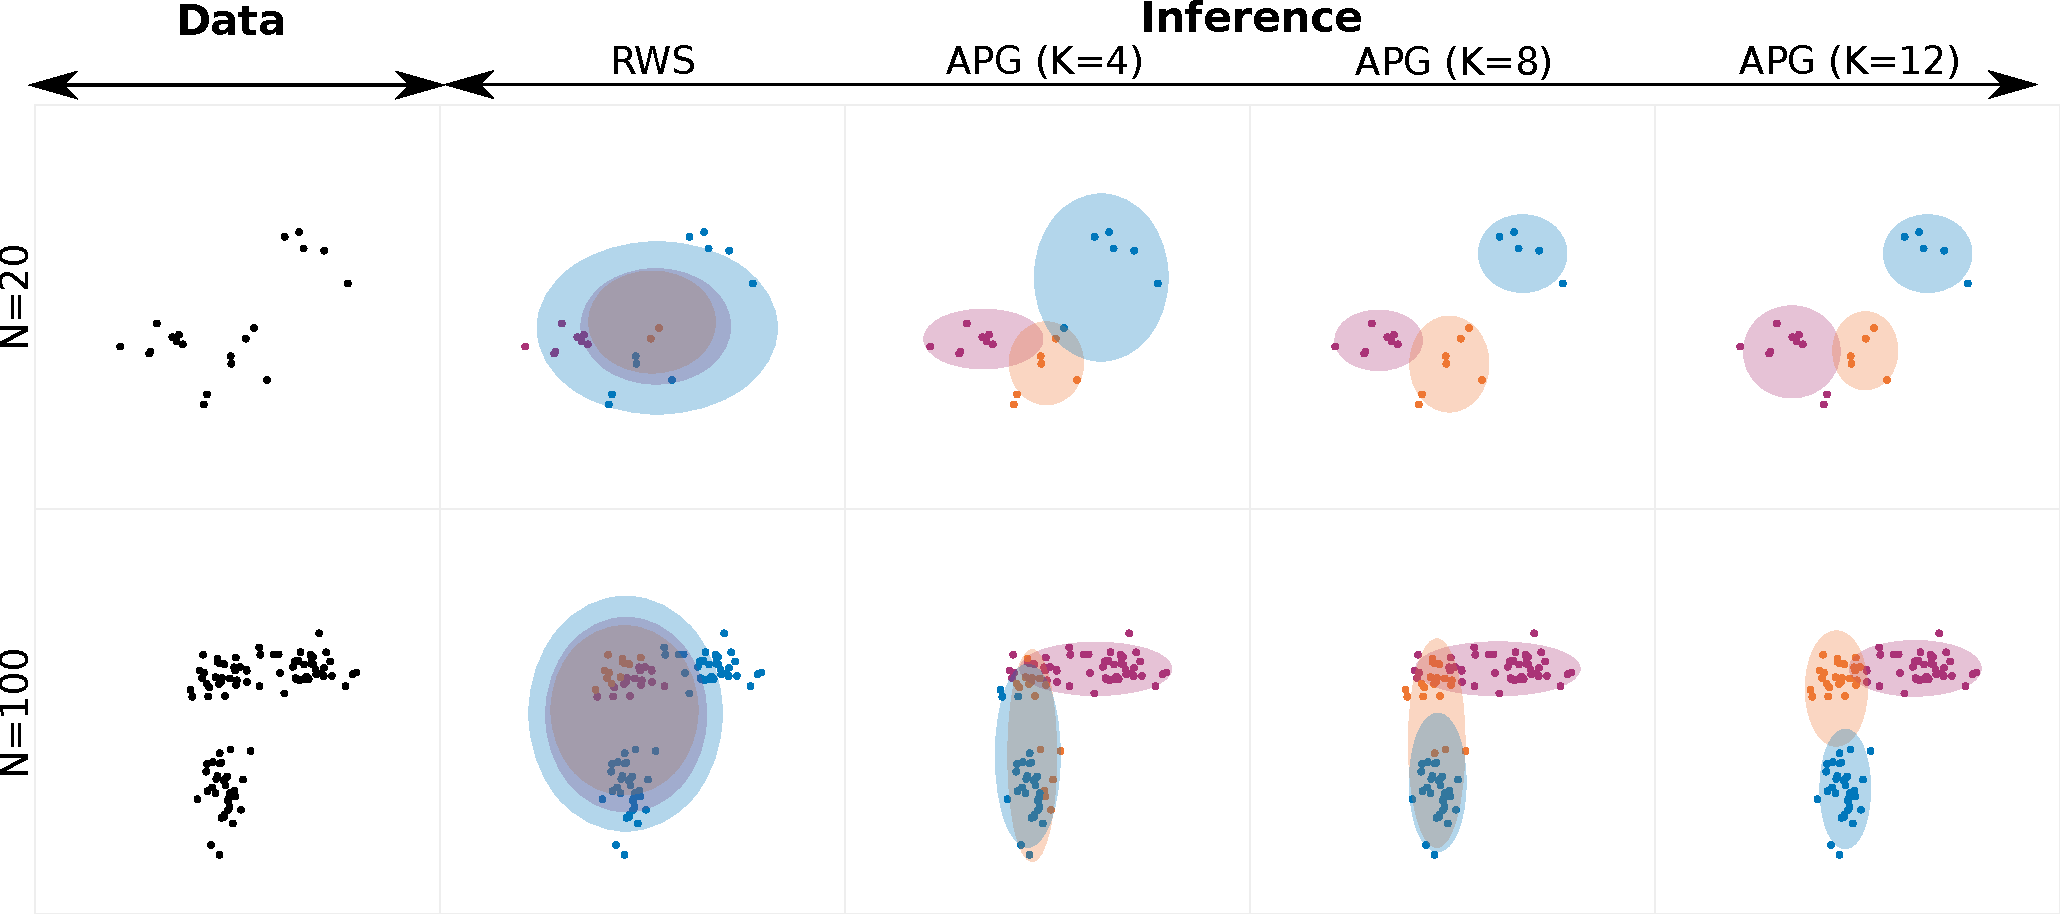
\includegraphics[width=85mm]{figures/gmm_samples_2datasets.pdf}
  \vspace*{-1mm}
  \caption{GMM}
  \label{fig:samples-gmm}
  \vspace{-1ex}
  \end{subfigure}%
  \begin{subfigure}[t]{0.5\textwidth}
  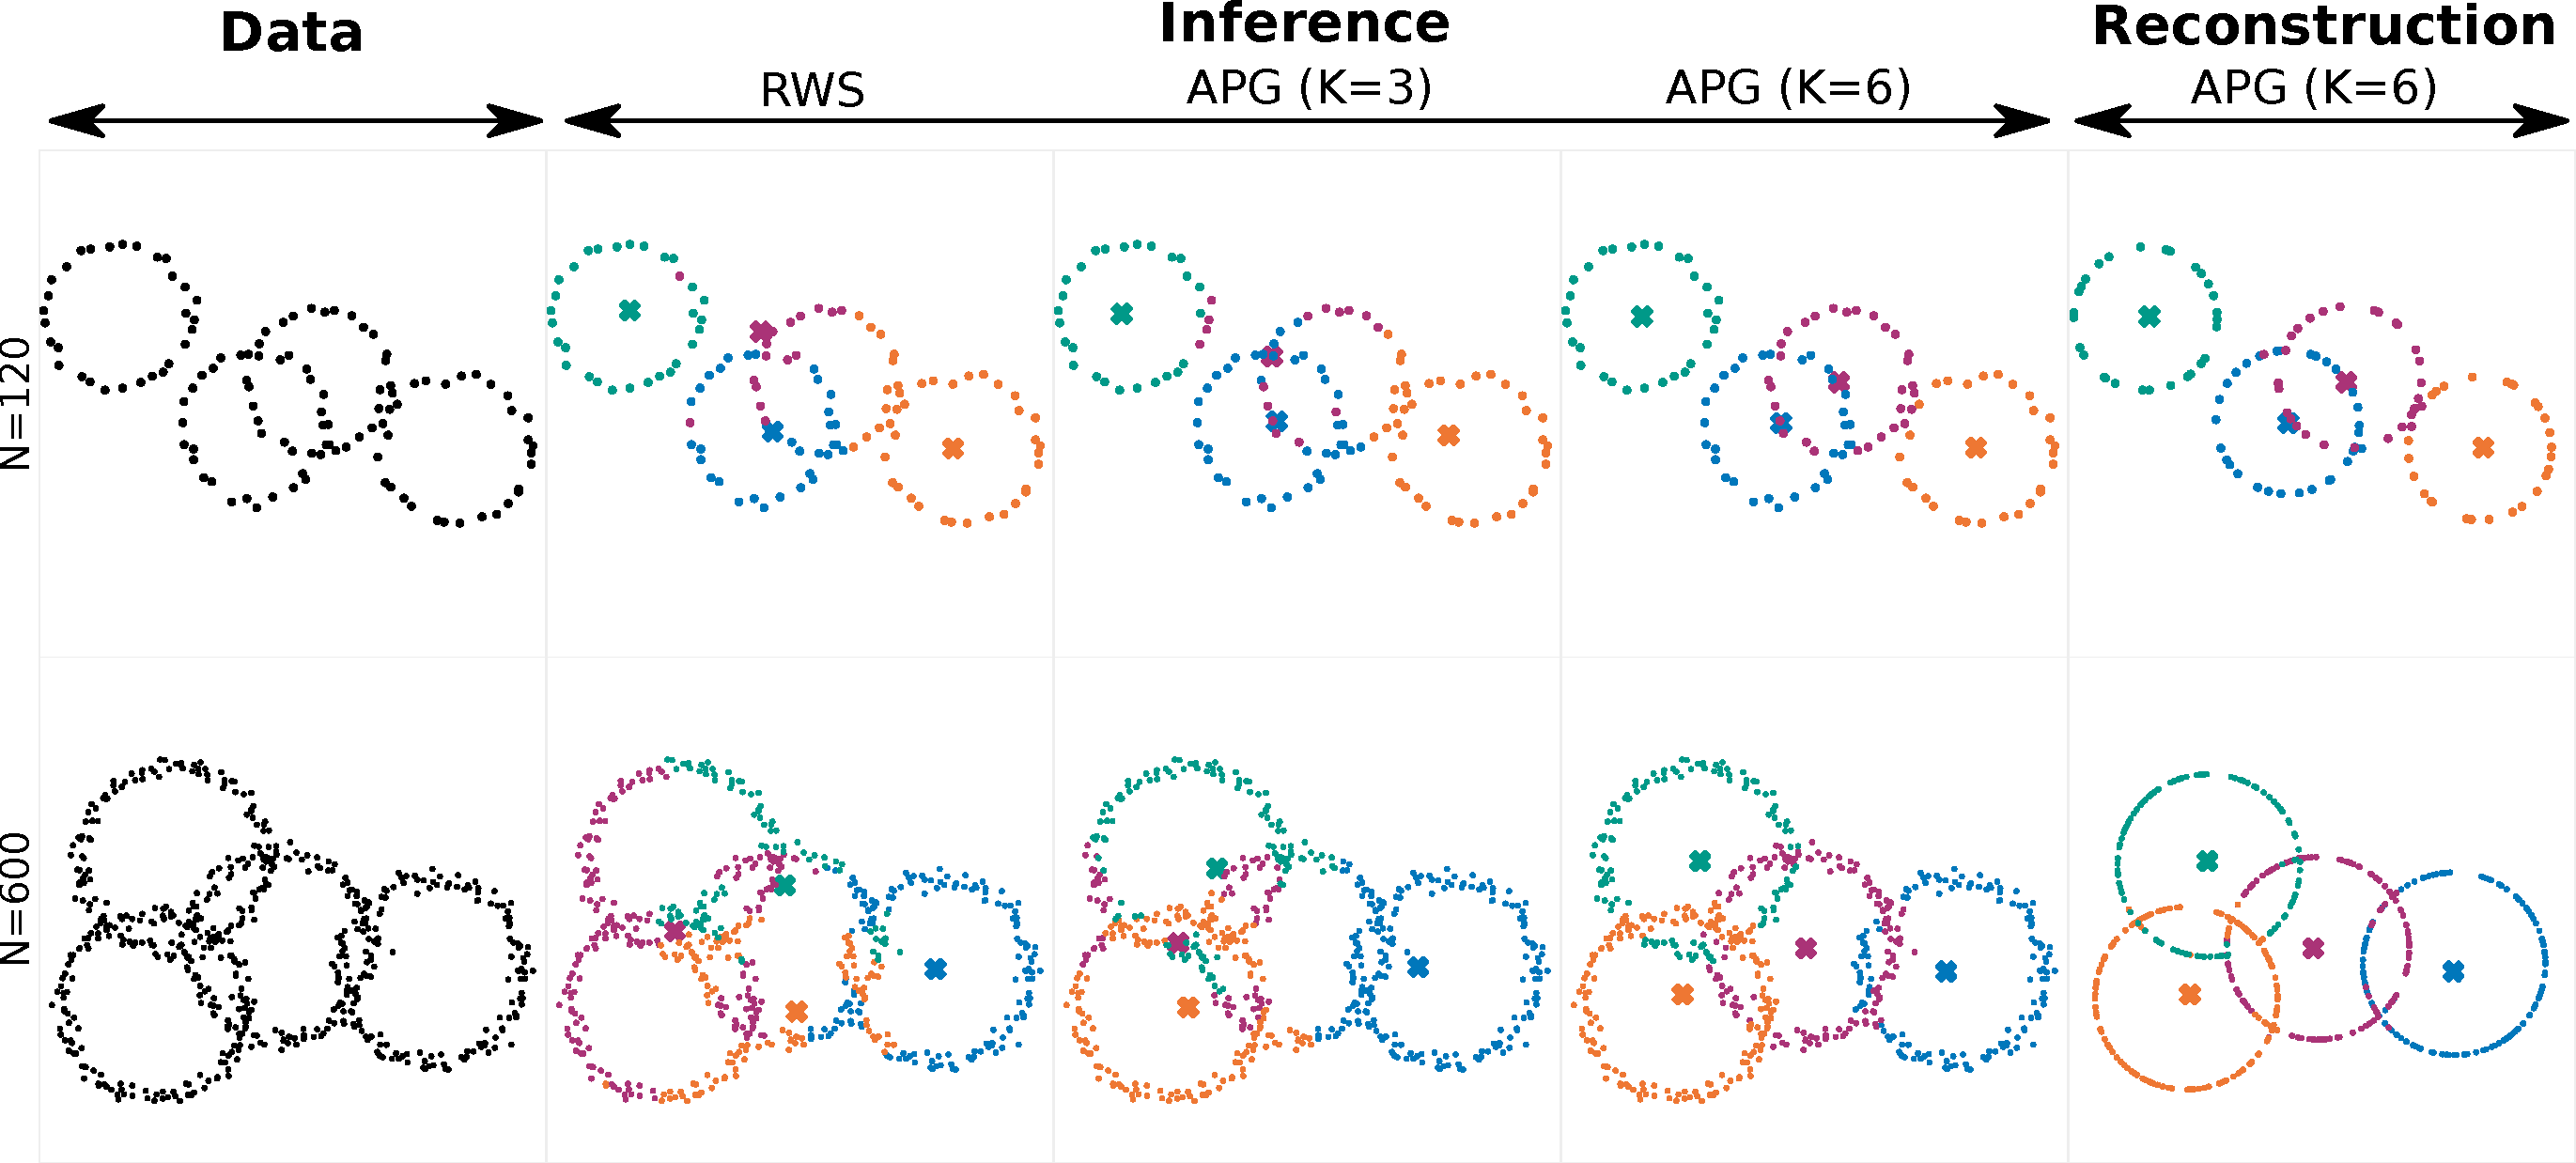
\includegraphics[width=85mm]{figures/dgmm_samples_2datasets.pdf}
  \vspace*{-1mm}
  \caption{DMM}
  \label{fig:samples-dgmm}
  \vspace{-1ex}
  \end{subfigure}
  \caption{Visualization of a single sample for (\textbf{a}) GMM instances with $N=100$ data points and (\textbf{b}) DMM instances with $N=600$ data points. The left columns show the data instance, the second column the inference result from RWS, and the subsequent columns the inference result after $K$ APG sweeps. In addition the rightmost column in (\textbf{b}) shows the reconstruction from the generative model.
  Unlike RWS, APG successfully learns the model parameters and an inference model and its perfomance improves with increasing $K$.}
  \vspace{-0.25em}
%   \caption{Visualization of a single sample for (\textbf{a}) a GMM instance with $N=100$ data points and (\textbf{b}) a DMM instance with $N=600$ data points. The left columns show the data instance, the second column the inference result from RWS, and the subsequent columns the inference result after $K$ APG sweeps. In addition the rightmost column in (\textbf{b}) shows the reconstruction from the generative model.}
  \label{fig:samples-mixture}
\end{figure*}

\vspace{-1.5em}
\section{Related Work}
\vspace{-0.25em}

Our work fits into a line of recent methods for deep generative modeling that seek to improve inference quality, either by introducing auxiliary variables~\cite{maaloe2016auxiliary, ranganath2016hierarchical}, or by performing iterative updates~\cite{marino2018iterative}. 
% Our specific approach to learning block proposals is related to a number of methods that, in some way or other, combine transition kernels with variational inference. 
Work by \citet{hoffman2017learning} applies Hamiltonian Monte Carlo to samples that are generated from the encoder, which serves to improve the gradient estimate w.r.t.~$\theta$ (Equation~\ref{eq:grad-theta}), while learning the inference network using a standard reparameterized ELBO objective. 
% Work by \citet{hoffman2017learning} applies Hamiltonian Monte Carlo methods to improve sample quality to obtain better gradient estimate w.r.t. the parameters of the generative model.
% While their inference network is 
% trained by maximizing a reparameterized ELBO 
% their architecture is
% specifically designed to introduce rotational invariance that can be exploited to speed up HMC.
% This renderes their approach inapplicable for large scale problems which require more specialized architectures where running standard HMC is computationally too expensive. 
% Li et al.~\cite{li2017approximate} consider learning an inference network which is used for initializing an MCMC chain. They focus on a setting where the density of the inference network cannot be evaluated.
% Learning is also performed by targeting the inclusive KL. However, the posterior expectation is approximated using MCMC and, due to the inability to compute the density, the gradient is estimated adversarially. 
\citet{li2017approximate} also use MCMC to improve the quality of samples from an encoder, but additionally use these samples to train the encoder by minimizing the inclusive KL divergence relative to the filtering distribution of the Markov chain. As in our work, the filtering distribution after multiple MCMC steps is intractable. \citet{li2017approximate} therefore use an adversarial objective to minimize the inclusive KL. Neither of these methods consider block decompositions of latent variables, nor do they learn kernels. 

\citet{salimans2015markov} derive a (stochastic) lower bound for variational inference which uses an importance weight defined in terms of forward and reverse kernels similar to Equation~\ref{eq:incremental-weight-forward-reverse}.
\citet{huang2018improving} extend the work by \citet{salimans2015markov} by learning a sequence of transition kernels that performs annealing from the initial encoder to the posterior. 
Since both these methods minimize an exclusive KL, rather than an inclusive KL, the gradient estimates rely on reparameterization which makes them inapplicable to models with discrete variables. 
Moreover, both methods perform a joint update on all variables while we are considering the task of learning conditional proposals.

%% russell amortized MCMC https://papers.nips.cc/paper/7669-meta-learning-mcmc-proposals.pdf
%% - learns block conditionals using sleep loss
%% - focus on conditional-sleep
\citet{wang2018meta} develop a meta-learning approach to learn Gibbs block conditionals. This work assumes a setup in which it is possible to sample $x, z$ from the true generative model $p(x,z)$. This circumvents the need for self-normalized estimators in Equation~\ref{eq:grad-self-normalized}, which are necessary when we additionally wish to learn the generative model. Similar to our work, the approach by \citet{wang2018meta} minimizes the inclusive KL, but uses the learned conditionals to define an (approximate) MCMC sampler, rather than using them as proposals in a SMC sampler. This work also has a somewhat different focus from ours, in that it primarily seeks to learn block conditionals that have the potential to generalize to previously unseen graphical models.


\vspace{-0.25em}
\section{Experiments}
\label{sec:experiments}

We evaluate APG samplers in 3 tasks. We begin by considering a Gaussian mixture model (GMM) as an exemplar of a model in the conjugate-exponential family. Here we verify that the learned proposals converge to conditional posterior, and show that APG can outperform other iterative inference methods even when using a smaller computational budget. We next consider a deep generative mixture model (DMM) that incorporates a neural likelihood. Here APG samplers can jointly train the generative model and inference model, and perform scalable inference to test-time instances with 600 points. 
% For both models we quantify performance in terms of the effective sample size (ESS) and the relative magnitude of the log joint.
In our third experiment, we consider an unsupervised model for multiple bouncing MNIST data. We extend the task proposed by \citet{srivastava2015unsupervised} to consider up to 5 individual digits, and learn both a deep generative model for videos and an inference model that performs tracking. At test time we show that APG easily scales beyond previously reported results for a specialized recurrent architecture \cite{kosiorek2018sequential}. 

Results on each of these tasks constitute a significant advance relative to the state of the art. APG is not only able to scale to models with higher complexity, but also provides a general framework for performing inference in models with global and local variables, which can be adapted to a variety of model classes with comparative ease. 


\subsection{Evaluating APG Samplers with Baselines}
In these 3 tasks we compare the APG samplers with multiple inference methods as baselines. The comparison is made under the same computation budget, which is defined as the number of times on evaluation of the log joint $p_\q(x, z)$. The first baseline is models trained by reweighted wake-sleep (RWS) methods, so that we can see the improvement by APG proposals. As RWSs are not iterative methods, we train and test the RWS baseline with $K \cdot L$ computation budget, same as the budget used in APG samplers.

As a means of assessing how much improvement achieved by the learned proposals, we implement the bootstrapped population sampler (BPS), which employs the exact APG sampling scheme but propose global (instance-level) variables from the prior $p(z)$. Since sampling from the prior is less likely to generate high-quality samples, we perform BPS with much more number of particles (i.e.~budget) within in the comparison.

Moreover we augment the RWS methods with 
\iffalse
all of which start with initial proposals learned in APG sampler (to make a fair comparison): (1) We apply true Gibbs sampling to verify that the learned proposals converge to conditional posterior. 
(2) We run bootstrapped population sampling (BPS) where we employ the APG sampling scheme but propose $\mu, \tau$ from the prior $p(\mu, \tau)$. This shows how much we improve by learning the proposals under the same sampling scheme. (3) We perform Hamiltonian Monte Carlo (HMC) method for continuous variables $\mu, \tau$ by marginalizing the discrete variables $c$, and Gibbs updates $p(c | x, \mu, \tau)$ for discrete variables.
Figure~\ref{fig:convergence-gmm} shows that the APG sampler outperforms even when we run HMC with 10 times the computation budget; And learned proposals substantially improves on inference since BPS does not converge even with 100 times budget.
\fi


\subsection{Gaussian Mixture Model}
\label{sec:gmm}
\vspace{-0.5em}
To evaluate whether APG samplers can learn the exact Gibbs updates in conditionally conjugate models, we consider a Gaussian mixture model 
\begin{align*}
    \mu_i, \tau_i &\sim \text{Normal-Gamma}(\mu_0, \nu_0, \alpha_0, \beta_0)
    , \,
    i =1,2..,I, \\
    c_n &\sim \mathrm{Cat}(\pi), \,
    x_n | c_n\!=\!i \sim \text{N}(\mu_i, 1 / \tau_i)
    , \,
    n =1,2,..,N.
\end{align*}
In this model, the global variables $z^\textsc{g} = \{\mu_{1:I}, \tau_{1:I}\}$ are the mean and precision for each mixture component, whereas the local variables are the cluster assignments $z^\textsc{l} = \{c_{1:N}\}$. Conditioned on cluster assignments, the Gaussian likelihood $p(\x_{1:N} \mid z_{1:N}, \mu_{1:I}, \tau_{1:I})$ is conjugate to a normal-gamma prior $p(\mu_{1:I}, \tau_{1:I})$ with sufficient statistics $T(x_n, c_n)$ 
\begin{align*}
    \Big\{\mathrm{I}[c_n \!=\! i], 
        ~\mathrm{I}[c_n \!=\! i] \: x_n, 
        ~\mathrm{I}[c_n \!=\! i] \: x_n^2 
        ~\Big\vert~ i \!=\! 1,2,\dots,I 
    \Big\}
    ,
\end{align*}
where $\mathrm{I}[z_n \!=\! i]$ is an indicator function that evaluates to 1 if the equality holds, and 0 otherwise.

\begin{table*}[t!]
\centering
\caption{$\log p_\q (x, z)$ averaged over test corpus for RWS, BPS, HMC-RWS, and Gibbs Sampling for different numbers of sweeps $K$.
We run HMC-RWS with 1, 5, and 10 leapfrog integration steps, which corresponds to 1, 5, and 10 times the computational budget used by APG with the same number of sweeps.
GMM's test corpus contains $20,000$ instances, each of which has $N=100$ data points. DMM's test corpus contains $20,000$ instances with $N=600$ data points per instance. Bouncing MNIST's test corpus contains $10,000$ instances each containing $T=100$ time steps and $D=5$ digits.
In all tasks, APG with $K=20$ performs the best.}
\vspace{0.5em}
\addtolength{\tabcolsep}{-2pt} 
\begin{tabularx}{\textwidth}{cccccccccc}
    \toprule
     & RWS & BPS & HMC-RWS & HMC-RWS & HMC-RWS & APG & APG & APG & GIBBS \\
     & & K=20 & K=20, LF=1 & K=20, LF=5 & K=5, LF=10 & K=5 & K=10 & K=20 & K=20 \\
    \midrule
    GMM ($\times10^2$)& $-7.651$ & $-6.688$ & $-6.594$ & $-5.420$ & $-4.673$ & $-4.816$ & $-4.556$ & $\textbf{-4.469}$ & $-4.573$ \\
    DMM ($\times10^3$) & $-3.172$ & $-4.204$ & $-2.185$ & $-2.184$ & $-2.184$ & $-2.050$ & $-2.040$ & $\textbf{-2.035}$ & -- \\
    BC-MNIST ($\times10^5$) & $-1.673$ & $-1.884$ & $-1.538$ & $-1.405$ & $-1.303$ & $-0.706$ & $-0.652$ & $\textbf{-0.620}$ & --\\
    \bottomrule
\end{tabularx}
\label{table:log-joint-all}
\end{table*}

We employ a variational distribution that initializes samples by $q_\f(\mu, c | x)$ and iterates over $q_\f(c \mid x, \mu, \tau)$ and $q_\f(\mu, \tau \mid x, c)$ , using point-wise neural sufficient statistics modeled after the ones in the analytical updates.
We train our model on 20,000 GMM instances, each containing $I = 3$ clusters and $N = 60$ data points, with $K=5$ sweeps, $L=10$ particles, $20$ instances per batch, learning rate $2.5\times10^{-4}$, and $2\times10^5$ gradient steps.
\begin{figure}[t!]
\centering
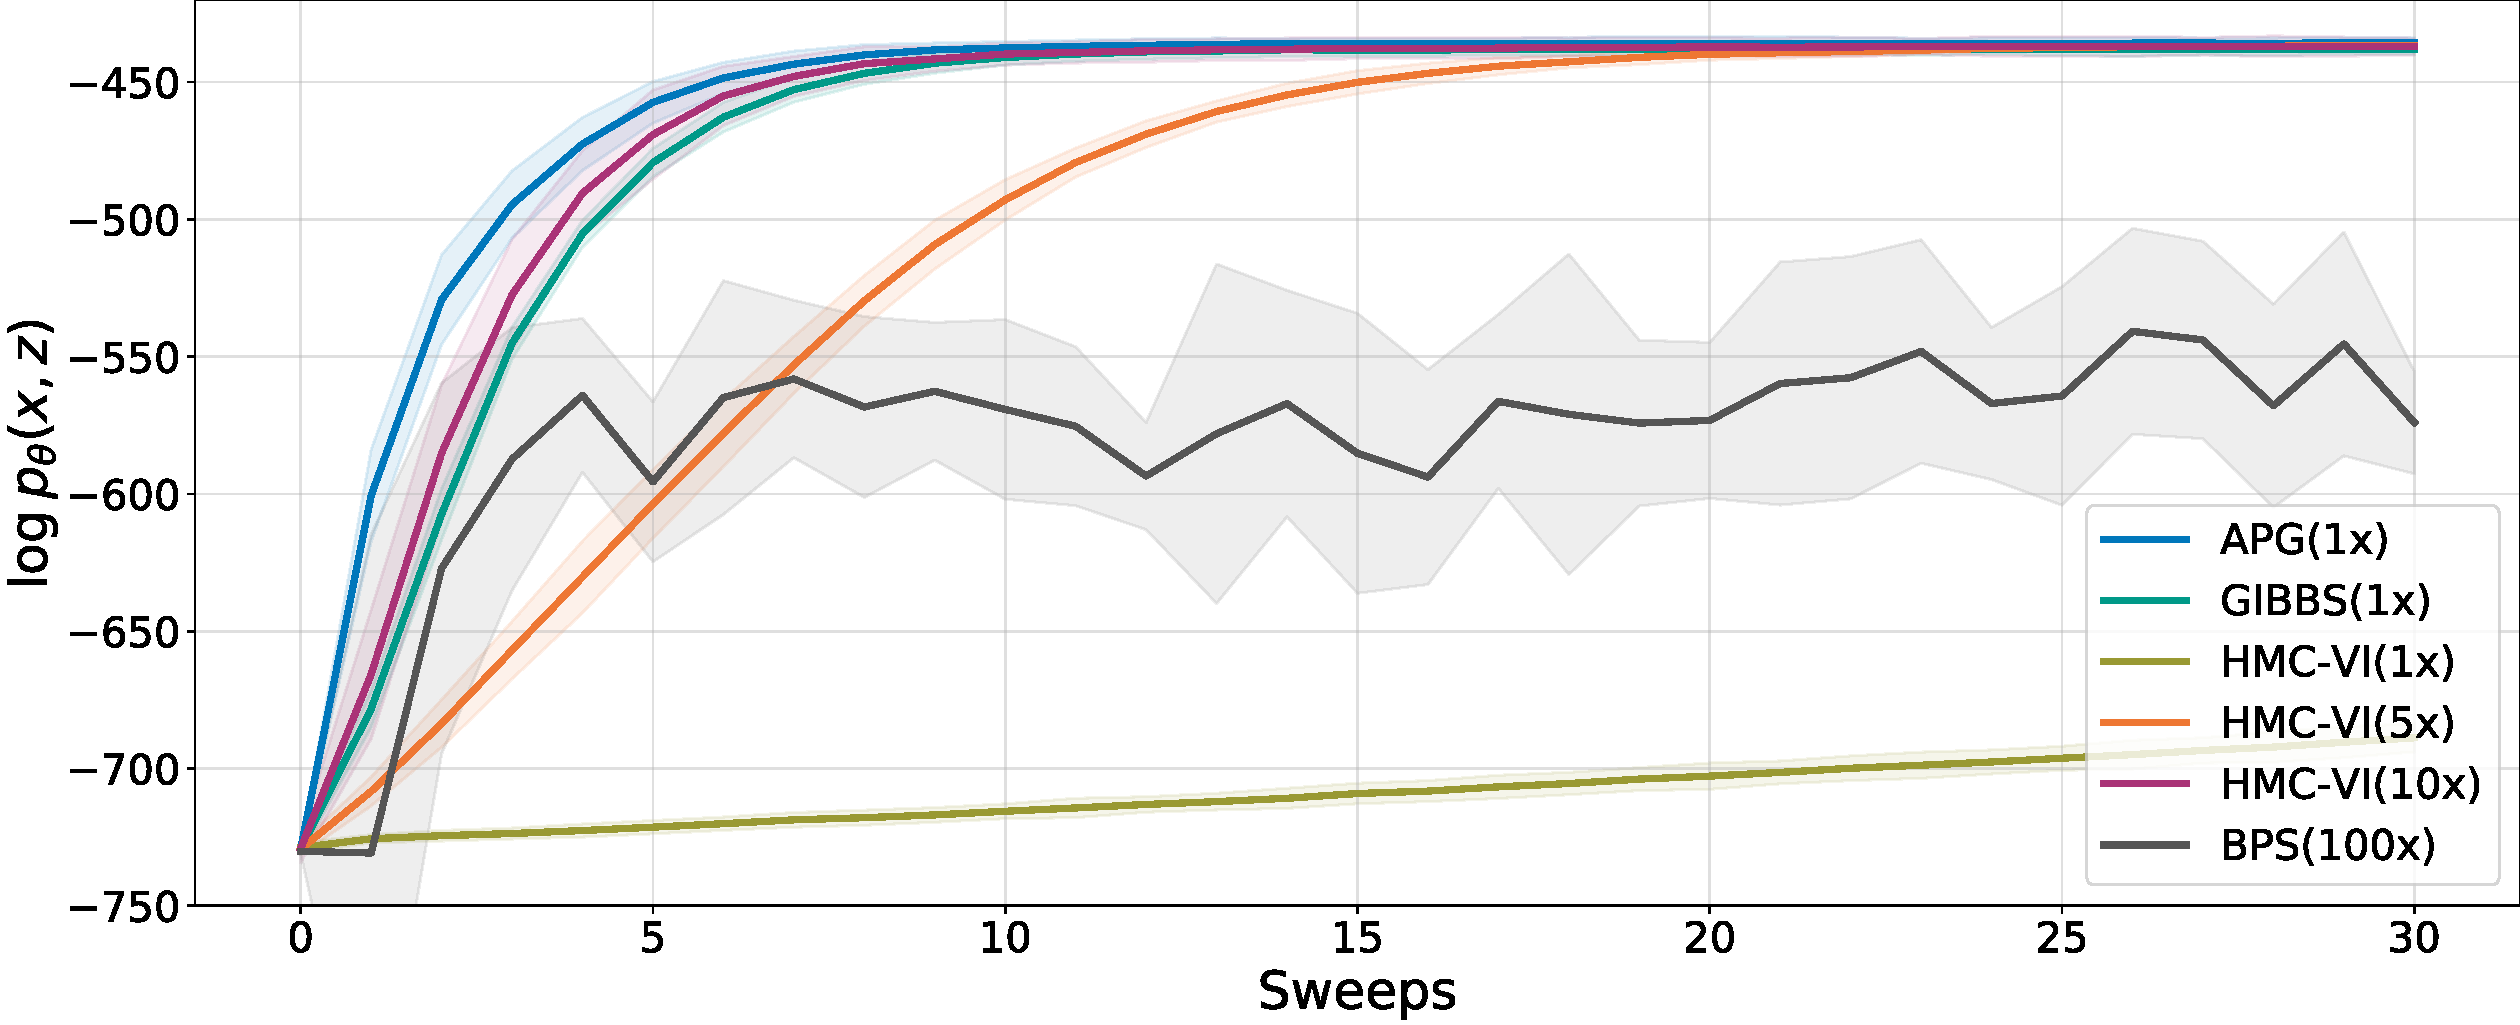
\includegraphics[width=\columnwidth]{figures/convergence_gmm_v2.pdf}
  \caption{$\log p_\theta(x, z)$ as a function of number of sweeps for a GMM test instance. We perform APG sampler and Gibbs sampler using $L=100$ particles, BPS using $L=10,000$ particles (around $100\times$ the computation budget), HMC-RWS using $L=100$ particles and $1, 5, 10$ leapfrog steps (around $1, 5, 10\times$ the computation budget), respectively. To achive results comparable to APG and Gibbs samplers, HMC-RWS needs a $10\times$ larger sampling budget while BPS underperforms even with a $100\times$ budget.}
  \label{fig:convergence-gmm}
\end{figure}
% We compare the APG sampler to samples from a standard encoder with MLP and LSTM architectures,  which is trained using reweighted wake-sleep (RWS). Both architectures are parameterized using the same neural sufficient statistics as the APG sampler.

Figure~\ref{fig:samples-gmm} shows a single sample in test instance with $N=100$ points. The sample is initialized from an RWS encoder and updated with APG sweeps. Even when using a parameterization that employs neural sufficient statistics, the RWS encoder fails to propose reasonable clusters, whereas the APG converges within 12 sweeps in GMM with more number of variables than training instances.



Furthermore, we compare the APG sampler with other iterative inference methods, all of which start with initial proposals learned in APG sampler (to make a fair comparison): (1) We apply true Gibbs sampling to verify that the learned proposals converge to conditional posterior. 
(2) We run bootstrapped population sampling (BPS) where we employ the APG sampling scheme but propose $\mu, \tau$ from the prior $p(\mu, \tau)$. This shows how much we improve by learning the proposals under the same sampling scheme. (3) We perform Hamiltonian Monte Carlo (HMC) method for continuous variables $\mu, \tau$ by marginalizing the discrete variables $c$, and Gibbs updates $p(c | x, \mu, \tau)$ for discrete variables.
Figure~\ref{fig:convergence-gmm} shows that the APG sampler outperforms even when we run HMC with 10 times the computation budget; And learned proposals substantially improves on inference since BPS does not converge even with 100 times budget.
\begin{figure}[t!]
\centering
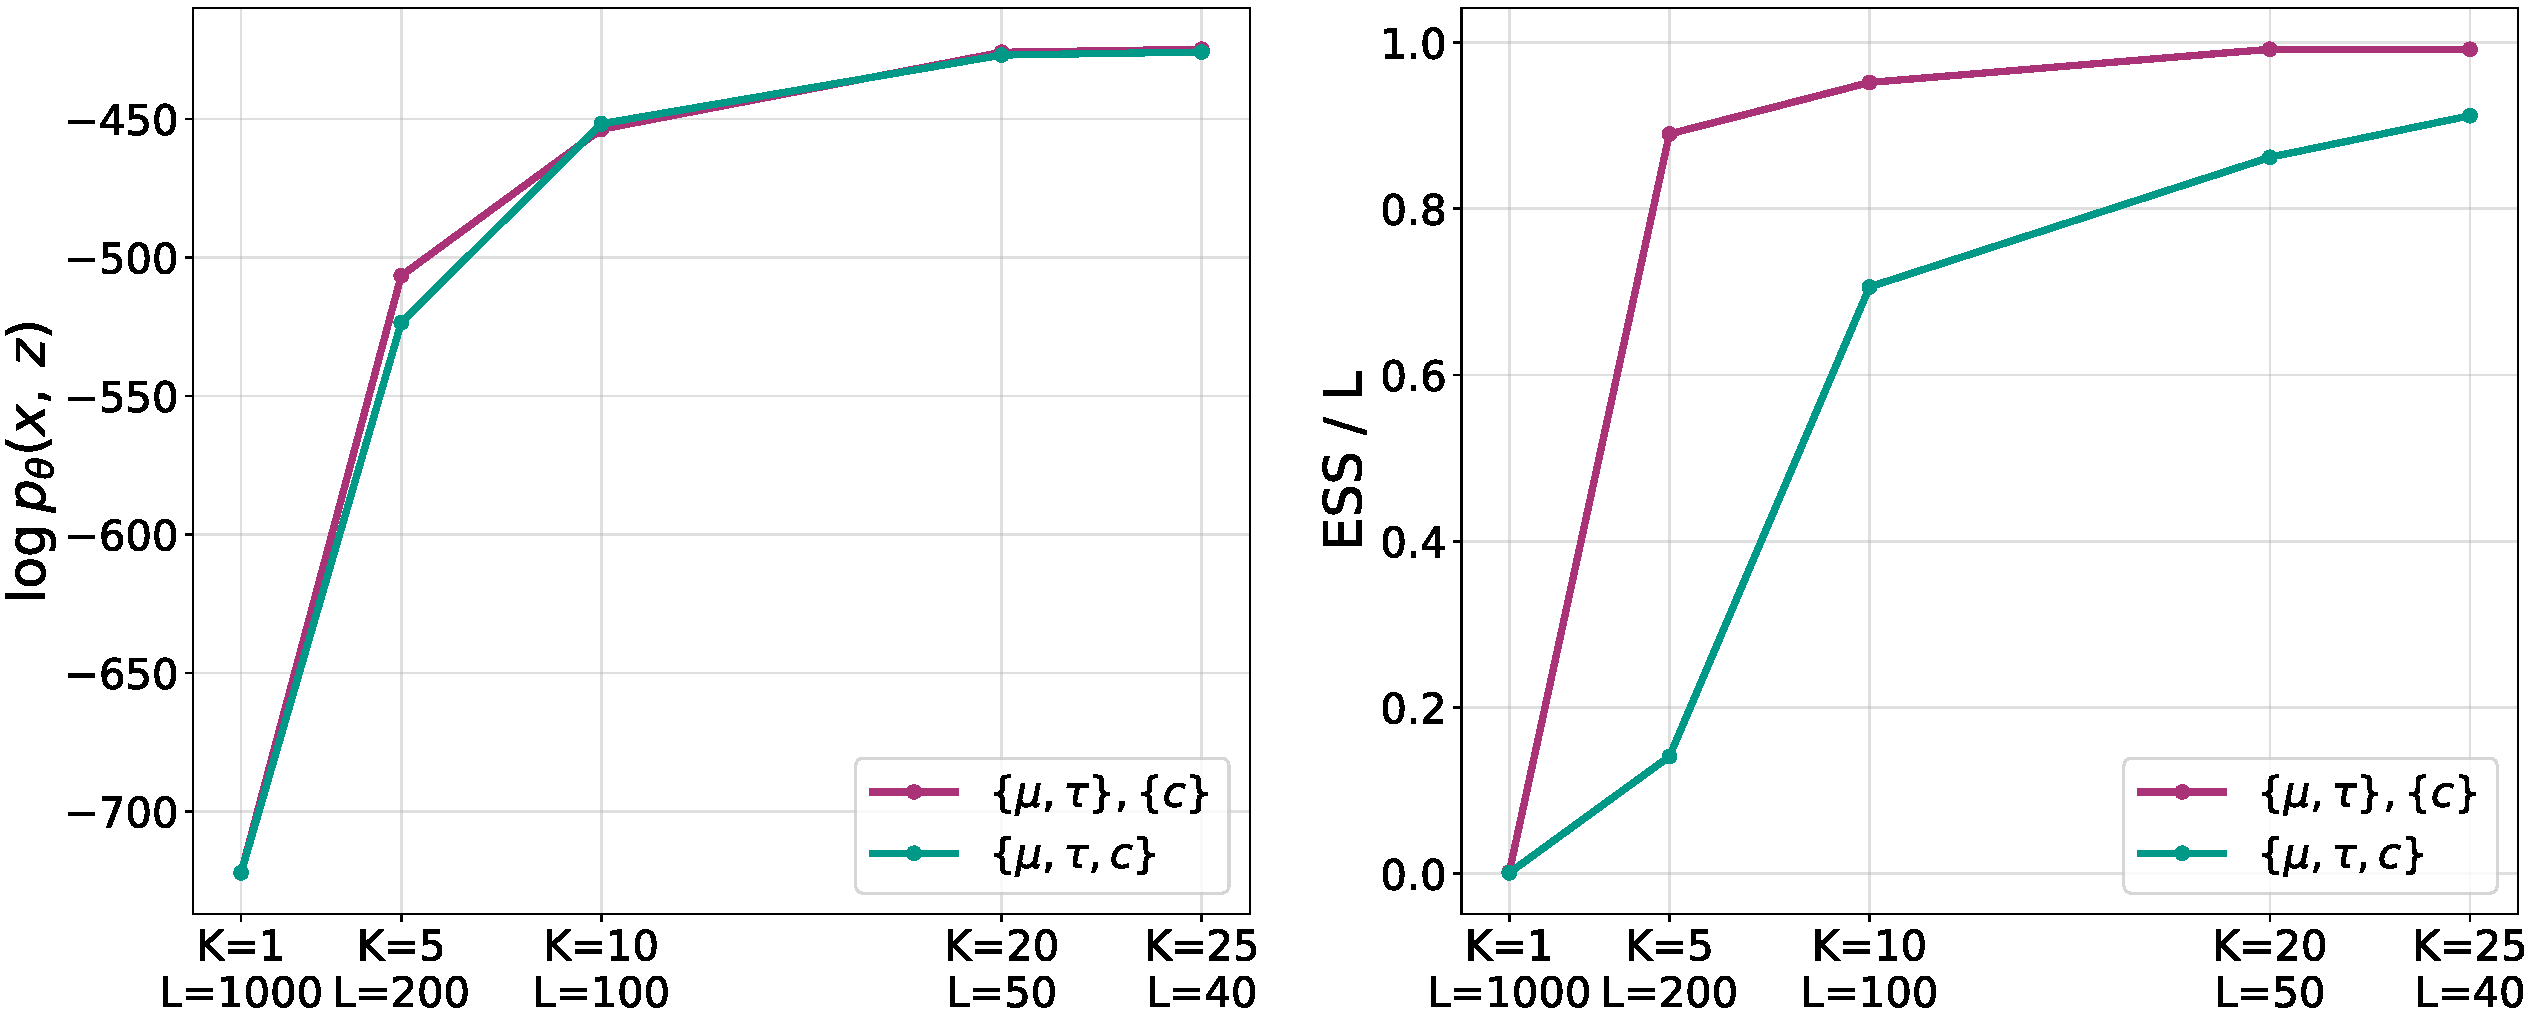
\includegraphics[width=\columnwidth]{figures/budget_gmm.pdf}
  \caption{$\log p(x, z)$ (left) and ESS (right) as a function of number of sweeps for APG samplers with different block update strategies and same overall sampling budget $K \cdot L = 1000$. A higher ESS is achieved by performing more sweeps with fewer samples.}
  \label{fig:fixed-budget-gmm}
\end{figure}

\begin{figure*}[!t]
  \centering
  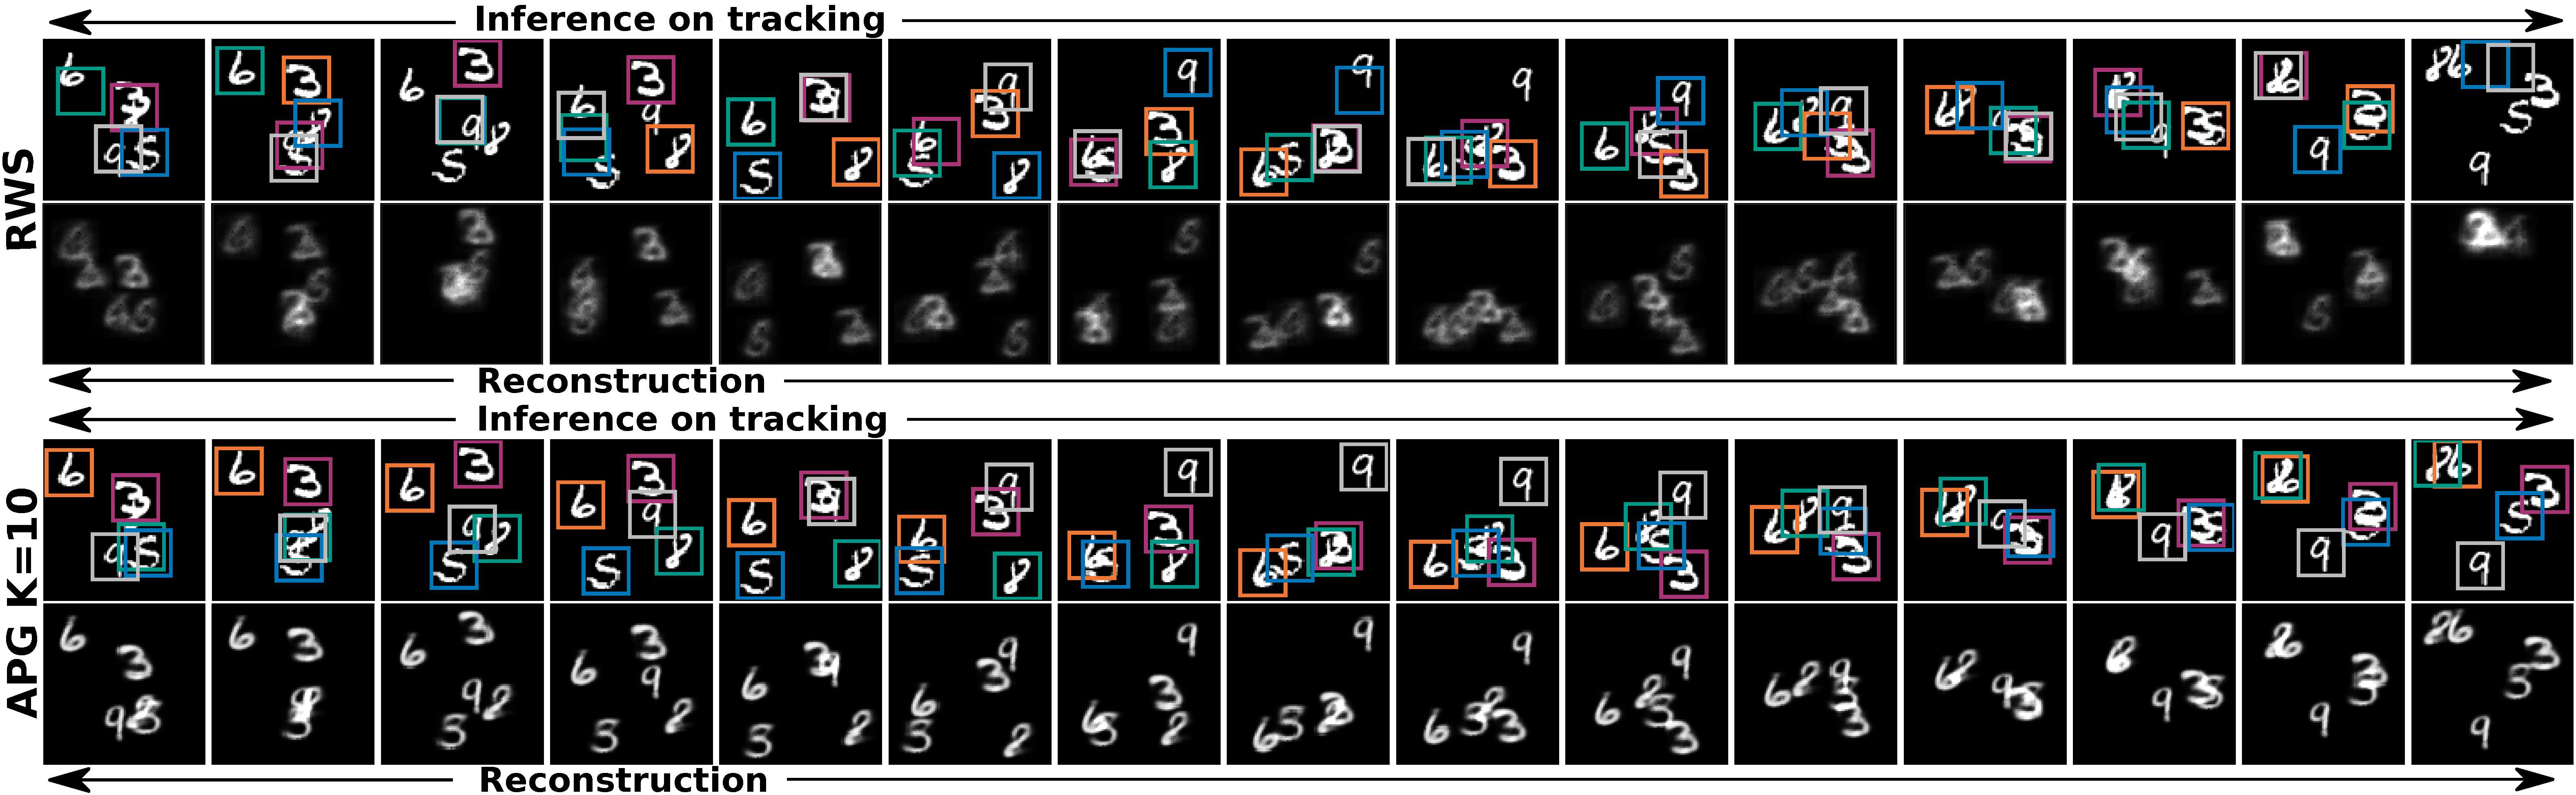
\includegraphics[width=1.0\textwidth]{figures/bmnist-5digits-samples-with-rws.pdf}
%   \vspace*{-5mm}
%   \caption{5 digits.}
%   \caption{Inferred trajectories (top), sequence reconstructions (bottom) and individual MNIST digit reconstructions (right) on one test set.}
%   \caption{A single sample after 10 APG sweeps in one video instance with $T=100$ time steps and $D=5$ digits. The visualization is truncated due to limited space (see Appendix~\ref{appendix:full-recons} for full time steps and Appendix~\ref{appendix:bmnist-comparison-rws} for more examples). Even when the digits are highly overlapped, APG sampler performs accurate inference on tracking, and the generative model can clearly reconstructs the video frames.}
  \caption{A single sample from variational distribution in one video instance with $T=100$ time steps and $D=5$ digits. The visualization is truncated by the first 15 time steps due to limited space (see Appendix~\ref{appendix:full-recons} for full time steps and Appendix~\ref{appendix:bmnist-comparison-rws} for more examples). The sample is initialized from RWS (top) and updated by $K=10$ APG sweeps (bottom). The APG sampler improves the inference results in tracking and also learns better MNIST digit embedding that gives better reconstruction.}
  \label{mnist-qualitative}
\end{figure*}


% \vspace{-1.0em}
% \begin{table*}[t!]
% \centering
% \caption{Average log joint $\log p_\q (x, z)$ over all test sets in each experiment. Iterative methods run with $K$ sweeps. }
% \begin{tabular}{cccccccccc}
% \toprule
%      & RWS & BPS & HMC1x & HMC5x & HMC10x & APG & APG & APG & GIBBS \\
%      & & K=20 & K=20 & K=20 & K=20 &  K=5 & K=10 & K=20 & K=20 \\
%     \midrule
%     GMM & -765.13 & -668.89 & -659.45 & -542.01 & -467.3 & -481.65 & -455.66 & -446.91 & -457.33 \\
%     DMM & -3172.0 & -4204.5 & -2184.9 & -2184.2 & -2184.0 & -2050.4 & -2040.2 & -2035.1 & -- \\
%     BouncingMNIST & -167390 & -188497 & -153850 & -140598 & -130354 & -70605 & -65224 & -62057 & --\\
%     \bottomrule
% \end{tabular}
% \label{table:log-joint-all}
% \end{table*}

We compare joint block updates $\{\mu, \tau, c\}$ with separate that decomposes blocks $\{\mu, \tau\}, \{c\}$, for varying number of sweeps (see Figure~\ref{fig:fixed-budget-gmm}). Here we compute the log joint distribution $\log p_\q(\x, z)$ as one metric, because the marginal $q_\f(z^k | x)$ is intractable% and it is hard to compute an lower/upper bound at each sweep. Also 
We additionally assess sample quality using the effective sample size
\vspace{-0.5em}
\begin{align*}
% \label{ess-eq}
    \frac{\text{ESS}}{L} 
    = 
    \frac{(\sum_{l=1}^L w^{k,l})^2}
         {L \sum_{l=1}^L (w^{k,l})^2}
    .
\end{align*}
% \vspace{-0.5em}
We can see that it is more effective to perform more sweeps $K$ with a smaller number of particles $L$ with fixed computation budget. Also we see that the decomposed block updates results in higher sample quality.

% that it is to increase the particle budget. To additionally evaluate different block update strategies we perform APG methods in GMM with two block updates; One that jointly update the global and local variables , and the other one that does it separately. We can see that the more granular sampling strategy improves the ESS.

\subsection{Deep Generative Mixture Model}
We next consider the task of jointly training a deep generative mixture model (DMM) $p_\q(\x, \z)$ with a inference model. Our data is a corpus of mixture models, each containing ring-shaped clusters. The generative model takes the form
\begin{align*}
    \mu_i &\sim \text{N}(0, 
    \sigma_0^2 \, I), 
    i = 1, 2, ..., I \\
    c_n &\sim \mathrm{Cat}(\pi), \alpha_n \sim \text{Beta}(1, 1), n = 1, 2, ..., N \\
    x_n | c_n=i &\sim \text{N}(g_\q(\alpha_n) + \mu_i, \sigma^2_{\epsilon} I).
\end{align*}
Here $\mu_i$ is center of the $i$th ring. Given a cluster assignment $c_n$ and an embedding $\alpha_n$ which goes into a MLP decoder $g_\q$, we sample a data point $x_n$ with 2D Gaussian noise. 

We employ a variational distribution that initializes samples by $q_\f(\mu, c, \alpha| x)$, and iterates over  $q_\f(c, \alpha | x, \mu)$ and $q_\f(\mu | x, c, \alpha)$. Using APG sampler, we train our model on 20,000 DMM instances, each containing $I = 4$ clusters and $N=200$ points, with $K=8$ sweeps, $L=10$ particles, 20 instances per batch, learning rate $10^{-4}$, and $3\times10^5$ gradient steps. (see Appendix \ref{appendix:architecture} for architecture).

Once again, we compare the APG sampler with the encoders using RWS. Figure~\ref{fig:samples-dgmm} shows visualization of a single sample from variational distribution in on DMM instance The APG sampler scales to a large range of number of variables, whereas a standard encoder trained using RWS fails to produce reasonable proposals.

\subsection{Time Series Model -- Bouncing MNIST}

Finally we consider the task of an unsupervised time series model, where our data is a corpus of video frames recording multiple bouncing MNIST digits. To demonstrate the scalability of APG samplers, we train both a deep generative model and a inference model with $60000$ video instances, each of which contains $T=10$ time steps and $D=3$ digits; Then we evaluate the model on test instances that contain $T=100$ time steps and $D=5$ digits. Our generative model has the form
%\vspace{-0.5em}
\begin{align*}
    z^{\mathrm{what}}_{d} 
    &\sim 
    \text{N}(0, I)
    ,
    \,
    z^{\mathrm{where}}_{d, 1} \sim \text{N}(0, I)
    ,
    \,
    d=1, 2,.., D,
    \\
    z^{\mathrm{where}}_{d, t} 
    %| z^{\mathrm{where}}_{d, t - 1} 
    &\sim 
    \text{Norm}(z^{\mathrm{where}}_{d, t - 1}, \sigma^2_0 I),
    \,
    t=1, 2,.., T,   
    \\
    x_t 
    %| z^\mathrm{where}_{d,t}, z^\mathrm{what}_d 
    &\sim
    \mathrm{Bern}
    \Big(
        \sigma
        \Big(
            \sum_{d} \mathrm{ST}
            \big(
                \mu_\theta(\z^{\mathrm{what}}_d), 
                z^{\mathrm{where}}_{d, t}
            \big)
        \Big)
    \Big)
\end{align*}
% \vspace{-0.5em}
where $\z_{1:D}^{\mathrm{what}}$ are the latent code of digits, and $\z_{1:D, 1:T}^{\mathrm{where}}$ are time-dependent positions. ST is a spatial transformer \cite{jaderberg2015spatial} that maps the output of a MLP decoder $\mu_\q$ that maps logits for a 28$\times$28 MNIST image onto a 96$\times$96 canvas based on $z^{\mathrm{where}}_{d, t}$. 
\begin{table}[t!]
    \centering
    \caption{Bouncing MNIST performance. Mean-squared error between test instance and its reconstruction across 5000 video instances with different number of time steps $T$ and digits $D$. We use a fixed sampling budget of $KL=1000$. APG samplers achieve substantial improvements relative to RWS and HMC-RWS.}
    \vspace{0.5em}
    \begin{tabularx}{\columnwidth}{ccccc}
    \toprule
        & RWS & HMC-RWS & APG & APG \\
        &  &  K=20, LF=10 & K=10 & K=20 \\
    \midrule
    D=5, T=20 & 265.1 & 261.2 & 117.7 & 103.8\\
    \hspace{0.5em}D=5, T=100 & 272.1 & 267.9  & 115.4 &  102.3\\
    %\hline
    D=3, T=20 & 134.0 & 124.1 & 60.4 & 58.9 \\   
    \hspace{0.5em}D=3, T=100 & 137.3 & 127.4 & 56.0 & 55.7 \\
    
    % & RWS & HMC10x & APG & APG \\
    % &  &  K=20 & K=10 & K=20 \\
    % \midrule
    % D=5, T=20 & 265.1 & 261.2 & 117.7 & 103.8\\
    % D=5, T=50 & 271.4 & 257.2 & 115.6 & 103.1 \\
    % \hspace{0.5em}D=5, T=100 & 272.1 & 267.9  & 115.4 &  102.3\\
    % %\hline
    % D=3, T=20 & 134.0 & 124.1 & 60.4 & 58.9 \\   
    % D=3, T=50 & 134.6 & 127.0 & 58.6 &  58.3 \\
    % \hspace{0.5em}D=3, T=100 & 137.3 & 127.4 & 56.0 & 55.7 \\
    \bottomrule
    \end{tabularx}
    \vspace{-1em}
    \label{table:mse-bmnist}
\end{table}

We employ a block update that decompose the variables into $T + 1$ blocks $(z_{1:D}^{\mathrm{what}}, z_{1:D, 1}^{\mathrm{where}}, z_{1:D, 2}^{\mathrm{where}}, \dotsc, z_{1:D, T}^{\mathrm{where}})$.
% Empirically this works better than splitting the latent variables into global and local variables, since resampling at each time step $t$ helps disentangle the digit locations if they overlap.
We train our model on 60000 bouncing MNIST instances, each containing $T=10$ time steps and $D=3$ digits, with $K=5$ sweeps, $L=10$ particles, $K=5$ instances per batch, learning rate $10^{-4}$, and $1.2\times10^7$ gradient steps (see Appendix \ref{appendix:architecture} for architecture).

Figure~\ref{mnist-qualitative} shows that the APG sampler achieves substantial inference and reconstruction results, and scales to test instances with 100s latent variables.

% Table~\ref{table:log-joint-all} shows the average log joint density $\log p_\q (x, z)$ over 10000 test-time video instances with $T=100$ time steps and $D =5$ digits. 

\vspace{-1.0em}
\section{Conclusion}
We introduce APG samplers, an adaptive importance sampling framework for amortized variational inference which iterates between updates to blocks of variables to train conditional proposals. To appropriately account for the size of the input data we developed a novel parameterization in terms of neural sufficient statistics inspired by sufficient statistics in conjugate exponential families.
We show that APG samplers can be used to efficiently train structured models with 100s of variables for state-of-the-art inference problems in an completely unsupervised manner and observe a substantial improvement of test-time inference compared to existing inference methods.

% One of the challenges in amortized inference for deep generative models is learning high-quality proposals for models with a structured prior over a high-dimensional set of latent variables. These priors arise naturally when, rather than encoding a single data point (e.g.~an image), we wish to encode a dataset (e.g.~a sequence of images). 
% Even for apparently simple problems, such as inferring the cluster parameters and assignments in a mixture model, standard encoders often fail to produce good samples. One of the reasons for this is that it is fundamentally difficult to jointly generate proposals for a high-dimensional set of latent variables.

% APG samplers are very general, and offer a path towards the development of deep generative models that incorporate structured priors to provide meaningful inductive biases in settings where we have little or no supervision. These methods have particular strengths in problems with global variables, but more generally make it possible to design amortized approaches that exploit conditional independence. Moreover, our parameterization in terms of neural sufficient statistics makes it comparatively easy to design models that scale to much larger number of latent variables and thus generalize to datasets that vary in size. 

% Immediate lines of future work are to compare the approach in this paper, which learns kernels that leave the target density invariant, with approaches that perform annealing, in which the learned kernels are assymmetric in the sense that they gradually transform the initial encoder distribution to the target density. 

% \section{Acknowledgements}

% This work was supported by the Intel Corporation, NSF award 1835309, the DARPA LwLL program, and startup funds from Northeastern University. Tuan Anh Le was supported by AFOSR award FA9550-18-S-0003.

\bibliography{icml-2020-references}
\bibliographystyle{icml2020}

\newpage
\appendix
\onecolumn
\icmltitle{Supplementary Material: Amortized Population Gibbs Samplers with Neural Sufficient Statistics}
\icmlkeywords{Machine Learning, ICML}
% \vskip 0.3in
\section{Gradient of the generative model}% $p_\q(x \mid z)$}
\label{appendix:grad-theta}
This is actually a known (although indeed not obvious) identity. Briefly, we can express the expected gradient of the log joint as
\begin{align*}
    \mathbb{E}_{p_\q(\z | \x)} 
    \left[
    \nabla_\q \log p_\q(\x, \z)
    \right]
    \mathbb{E}_{p_\q(\z | \x)} 
    \left[
    \nabla_\q \log p_\q(\x) + \nabla_\q \log p_\q(\z | \x)
    \right]
    \mathbb{E}_{p_\q(\z | \x)} 
    \left[
    \nabla_\q \log p_\q(\x) 
    \right]
    \nabla_\q \log p_\q(\x)
\end{align*}
Here we make use of a standard identity that is also used in, e.g., likelihood-ratio estimators
\begin{align*}
\mathbb{E}_{p_\q(\z | \x)}
\left[
    \nabla_\q \log p_\q(\z | \x)
\right] 
=
\int p_\q(\z | \x) \nabla_\q \log p_\q(\z | \x) \: dz
=
\int \nabla_\q p_\q(\z | \x) \: dz
=
\nabla_\q \int p_\q(\z | \x) \: dz
=
\nabla_\q 1
= 
0
\end{align*}
Therefore, we have the the following equality
\begin{align*}
\nabla_\q \log p_\q(\x) 
= 
\mathbb{E}_{p_\q(\z | \x)} 
\left[
\nabla_\q \log p_\q(\x, \z)
\right].
\end{align*}
which is Equation ~\ref{eq:grad-theta}. As a result, we can then use self-normalized importance sampling to approximate     $\mathbb{E}_{p_\q(\z | \x)} \left[\nabla_\q \log p_\q(\x, \z) \right]$.

\section{Importance weights in sequential importance sampling}
\label{appendix:sis-weight}
At step $k=1$, we use exactly the standard importance sampler, thus it is obvious that the following is a valid importance weight
\begin{align*}
    w^1 = \frac{\gamma^1(z^1)}{q^1(z^1)}.
\end{align*}
When step $k>2$, we are going to prove that the importance weight relative to the intermediate densities has the form
\begin{align}
    \label{appendix:eq:sis-weight}
    w^k
    = 
    \frac{\gamma^k(z^{1:k})}
         {q^1(z^1) \prod_{k'=2}^k q^{k'}(z^{k'} \mid z^{1:k'-1})}.
\end{align}

At step $k=2$, the importance weight is defined as 
\begin{align*}
    w^k 
    &= 
    v^{2} \: w^1
    \: =
    \frac{\gamma^2(z^{1:2})}{\gamma^{1}(z^{1})\:q^2(z^2 \mid z^{1})} \frac{\gamma^1(z^1)}{q^1(z^1)}
    \: = \frac{\gamma^2(z^{1:2})}{q^1(z^1) \: q^2(z^2 \mid z^{1})}.
\end{align*}
which is exactly that form. Now we prove weights in future steps by induction. At step $k\geq 2$, assume the weight has the form in Equation~\ref{appendix:eq:sis-weight}, i.e.
\begin{align*}
    w^k
    = 
    \frac{\gamma^k(z^{1:k})}
         {q^1(z^1) \prod_{k'=2}^k q^{k'}(z^{k'} \mid z^{1:k'-1})}.    
\end{align*}
then at step $k+1$, the importance weight is the product of incremental weight and incoming weight 
\begin{align*}
    w^{k+1}
    =
    v^{k+1} \: w^k
    =
    \frac{\gamma^{k+1}(z^{1:k+1})}{\gamma^{k}(z^{1:k})\:q^{k+1}(z^{k+1} \mid z^{1:k})}
    \frac{\gamma^k(z^{1:k})}
         {q^1(z^1) \prod_{k'=2}^k q^{k'}(z^{k'} \mid z^{1:k'-1})}
    =
    \frac{\gamma^{k+1}(z^{1:k+1})}{q^1(z^1) \prod_{k'=2}^{k+1} q^{k'}(z^{k'} \mid z^{1:k'-1})}
    .    
\end{align*}
Thus the importance weight $w^k$ has the form of Equation~\ref{appendix:eq:sis-weight} at each step $k>2$ in sequential importance sampling.
\section{ Derivation of Posterior Invariance}
\label{appendix:posterior-invariance}
We can see that individual block updates leave the posterior invariant by proposing variables $\z^k_{\preceq b}$ from a partial kernel $\kappa(\z^k_{\preceq b} \mid x, \z^{k-1})$ and then marginalize over the corresponding variables from the previous step $\z^{k-1}_{\preceq b}$,
\begin{align*}
    \int 
    dz^{k-1}_{\preceq b} 
    \:
    p_\q(\z^{k-1} \mid \x) 
    \: 
    \kappa(\z^k_{\preceq b} \mid x, \z^{k-1}) 
    %\\
    %&= 
    &=
    \int 
    dz^{k-1}_{\preceq b} 
    \:
    p_\q(\z^{k-1} \mid \x) 
    \: 
    \int dz^k_{\succ b}
    \:
    \kappa(\z^k \mid x, \z^{k-1})
    \\
    &= 
    \int 
    dz^{k-1}_{\preceq b} 
    \: 
    p_\q(\z^{k-1} \mid x)
    \prod_{m=1}^b p_\q(\z^k_m \mid \x, \z^{k}_{\prec m}, \z^{k-1}_{\succ m})
    \\
    &=
    \int 
    dz^{k-1}_{\preceq b} 
    \: 
    p_\q(\z^{k-1} \mid \x)
    p_\q(\z^k_{\preceq b} \mid \x, \z^{k-1}_{\succ 1})
    \\
    %&=
    %\int d\z^{k-1}_{\preceq b} 
    %\: p_\q(\z^k_{\preceq b}, \z^{k-1} \mid \x)\\
    &=
    p_\q(\z^k_{\preceq b}\:, \: \z^{k-1}_{\succ b} \mid \x)
    .
\end{align*}

\section{Resampling Algorithm}
\label{appendix:resample-algo}
\begin{algorithm}[!t]
    \setstretch{1.2}
  \caption{\textsc{resample}}
  \label{alg:resample}
\begin{algorithmic}[1]
\small
  \State \textbf{Input:} $z^{\:1:L}, w^{\:1:L}$
  \State \textbf{Output:} $z'^{\:1:L}, w'^{\:1:L}$
  \For {$i = 1$ \textbf{to} $L$}
    \State $a^i \sim \mathrm{Disc}(\{w^l / \sum_{l' = 1}^L w^{l'}\}_{l=1}^L)$\Comment{Index Selection} 
    % \State $P(a^i = l) = w^l / \sum_{l' = 1}^L w^{l'}$
    \State Set $ z'^{\:i} = z^{a^i}$
    \State Set $ w'^{\:i} = \frac{1}{L} \sum_{l = 1}^L w^l$\Comment{Re-Weigh}
    \EndFor
  \State \textbf{Return} $z'^{\:1:L}, w'^{\:1:L}$
\end{algorithmic}
\end{algorithm}

\begin{algorithm}[!t]
  \setstretch{1.2}
  \caption{\textsc{Systematic Resampling}}
  \label{alg:resampling_sys}
\begin{algorithmic}[1]
\small
    \State \textbf{Input:} $z^{\:1:L}, w^{\:1:L}$
    \State \textbf{Output:} $z'^{\:1:L}, w'^{\:1:L}$
%   \State{Sort weights (optional)}
    \State{$u \sim \mathcal{U}[0,1)$}
    \State{$W^{1:L} = \textsc{Inclusive-Prefix-Sum}(w^{1:L})$}
    \For {$i = 1$ \textbf{to} $L$}
        \State $r_i = \frac{N W^i}{W^L}$
        \State Set $O^i = \min(L, \left\lfloor r_i + u \right\rfloor)$ \Comment{compute comulative offspring} 
    \EndFor
    \State Set $O^0 = 0$
    \For {$i = 1$ \textbf{to} $L$}
        \State Set $o^i= O^i - O^{i-1}$
        \For {$j = 1$ \textbf{to} $o_i$} \Comment{Convert to ancestors}
            \State Set $a^{O^{i-1} + j} = i$
    \EndFor
    \State Set $z'^{\:i} = z^{a^i}$
    \State Set $w'^{\:i} = \frac{1}{L} \sum_{l = 1}^L w^l$ \Comment{Re-Weigh}
    \EndFor
    \State \textbf{Return} $z'^{\:1:L}, w'^{\:1:L}$
\end{algorithmic}
\end{algorithm}
% https://arxiv.org/pdf/1301.4019.pdf

\section{Proof of the amortized population Gibbs algorithm}
\label{appendix:proof-algo}

Here, we provide an alternative proof of correctness of the APG algorithm given in Algorithm~\ref{alg:amortized-gibbs}, based on the construction of proper weights~\cite{naesseth2015nested} which was introduced after SMC samplers~\cite{delmoral2006sequential}.
We first introduce proper weights, and then present several operations that preserve the proper weighting property and finally we apply these properties in proving correctness of APG.

\subsection{Proper weights}

\begin{definition}[Proper weights]
    Given an unnormalized density $\tilde p(z)$, with corresponding normalizing constant $Z_p := \int \tilde p(z) \,\mathrm dz$ and normalized density $p \equiv \tilde p / Z_p$, the random variables $z, w \sim P(z, w)$ are properly weighted with respect to $\tilde p(z)$ if and only if for any measurable function $f$
    \begin{align}
    \label{eq:pw}
    \E_{P(z, w)}\left[w f(z)\right] = Z_p \E_{p(z)}[f(z)]. 
    \end{align}
    We will also denote this as
    \begin{align*}
        z, w \pw \tilde p.
    \end{align*}
\end{definition}

\paragraph{Using proper weights.}
Given independent samples $z^l, w^l \sim P$, we can estimate $Z_p$ by setting $f \equiv 1$:
\begin{align*}
    Z_p \approx \frac{1}{L} \sum_{l = 1}^L w^l.
\end{align*}
This estimator is unbiased because it is a Monte Carlo estimator of the left hand side of \eqref{eq:pw}.
We can also estimate $\E_{p(z)}[f(z)]$ as
\begin{align*}
    \E_{p(z)}[f(z)] \approx \frac{\frac{1}{L} \sum_{l = 1}^L w^l f(z^l)}{\frac{1}{L} \sum_{l = 1}^L w^l}.
\end{align*}
While the numerator and the denominator are unbiased estimators of $Z_p \E_{p(z)}[f(z)]$ and $Z_p$ respectively, their fraction is biased.
We often write this estimator as
\begin{align}
    \E_{p(z)}[f(z)] \approx \sum_{l = 1}^L \bar w^l f(z^l), \label{eq:pw-estimation}
\end{align}
where $\bar w^l := w^l / \sum_{l' = 1}^L w^{l'}$ is the normalized weight.

\subsection{Operations that preserve proper weights}


\begin{proposition}[Nested importance sampling]
    Adapted from \cite[Algorithm 1]{naesseth2015nested}.
    Given unnormalized densities $\tilde q(z), \tilde p(z)$ with the normalizing constants $Z_q, Z_p$ and normalized densities $q(z), p(z)$, if 
    \begin{align}
        z, w \pw \tilde q, \label{eq:1}
    \end{align}
    then
    \begin{align*}
        z, \frac{w\tilde p(z)}{\tilde q(z)} \pw \tilde p.
    \end{align*}
\end{proposition}
\begin{proof}
    First define the distribution of $z, w$ as $Q$.
    For measurable $f(z)$
    \begin{align*}
        \E_{Q(z, w)}\left[\frac{w\tilde p(z)}{\tilde q(z)} f(z)\right] 
        = Z_q \E_{q(z)}\left[\frac{\tilde p(z) f(z)}{\tilde q(z)}\right]
        = Z_q \int q(z) \frac{\tilde p(z) f(z)}{\tilde q(z)} \,\mathrm dz
        = \int \tilde p\textbf{}(z) f(z) \,\mathrm dz
        = Z_p \E_{p(z)}[f(z)].
    \end{align*}
\end{proof}

\begin{proposition}[Resampling]
\label{proposition:resampling}
    Adapted from [Section 3.1] \cite{naesseth2015nested}.
    Given an unnormalized density $\tilde p(z)$ (normalizing constant $Z_p$, normalized density $p(z)$), if we have a set of properly weighted samples
    \begin{align}
        z^l, w^l \pw \tilde p,  \quad l = 1,\ldots, L \label{eq:bla}
    \end{align}
    then the resampling operation preserves the proper weighting, i.e.
    \begin{align*}
        z'^{\:l}, w'^{\:l} \pw \tilde p, \quad l = 1,\ldots, L
    \end{align*}
    where $z'^{\:l} = z^{a}$ with probability $P(a = i) = w^i / \sum_{l=1}^L w^l$ and $w'^{\:l} := \frac{1}{L} \sum_{l = 1}^L w^l$.
\end{proposition}
\begin{proof}
    Define the distribution of $z^l, w^l$ as $\hat{P}$.
    We show that for any $f$, $\E[f(z^{a}) w'^{\:l}] = Z_p \E_{p(z)}[f(z)]$.
    \begin{align*}
    &
        \E_{\left(\prod_{l=1}^L \hat{P}(z^l, w^l)\right) p(a \mid w^{1:L})} \bigg[f(z^{a}) w'^{l}\bigg] \\
        &= \E_{\prod_{l=1}^L \hat{P}(z^l, w^l)}\left[\sum_{i = 1}^L f(z^i) w' \: P(a = i)\right]  \\
        &= \E_{\prod_{l=1}^L \hat{P}(z^l, w^{l})}\left[\sum_{i = 1}^L f(z^i) w'  \frac{w^i}{ \sum_{l'=1}^L w^{l'}}\right]  \\
        &= \E_{\prod_{l=1}^L \hat{P}(z^l, w^l)}\left[\frac{1}{L}\sum_{i = 1}^L f(z^i) w^i\right] \\
        &= \frac{1}{L}\sum_{i = 1}^L \E_{\hat{P}(z^i, w^i)}\left[f(z^i) w^i\right]
        = \frac{1}{L}\sum_{i = 1}^L Z_p \E_{p(z)}[f(z)]
        = Z_p \: \E_{p(z)}[f(z)]. 
    \end{align*}
\end{proof}
Therefore, the resampling will return a new set of samples that are still properly weighted relative to the target distribution in the APG sampler (Algorithm~\ref{alg:amortized-gibbs}).
\begin{proposition}[Move]
\label{proposition:extendedspace}
    Given an unnormalized density $\tilde p(z)$ (normalizing constant $Z_p$, normalized density $p(z)$) and normalized conditional densities $q(z' \given z)$ and $r(z \given z')$, the proper weighting is preserved if we apply the transition kernel to a properly weighted sample, i.e.~if we have
    \begin{align}
        &
        z^l, w^l \pw \tilde p, \label{eq:pw-of-p}\\[1em]
        &
         z'^{\:l} \sim q(z'^{\:l} \given z^l),  \label{eq:z-prime}\\[1em]
        &
        w'^{\:l} = \frac{\tilde p(z'^{\:l})r(z^l \given z'^{\:l})}{\tilde p(z^l)q(z'^{\:l} \given z^l)} w^l, \qquad l = 1, \ldots, L \label{eq:w-prime}
    \end{align}
%     \noindent\begin{subequations} 
%     \begin{tabularx}{\textwidth}{@{}XXX@{}}
%         \begin{equation}
%             z, w \pw \tilde p, \label{eq:pw-of-p}
%         \end{equation}&
%         \begin{equation}
%             z' \sim q(z' \given z), \label{eq:z-prime}
%         \end{equation}&
%         \begin{equation}
%             w' = \frac{\tilde p(z')r(z \given z')}{\tilde p(z)q(z' \given z)} w, \label{eq:w-prime}
%         \end{equation}
%     \end{tabularx}
%   \end{subequations} 
then we have
    \begin{align}
        z'^{\:l}, w'^{\:l} \pw \tilde p, \qquad  l = 1, \ldots, L \label{eq:to-prove}
    \end{align}
\end{proposition}
\begin{proof}
    Firstly we simplify the notation by dropping the superscript $l$ without loss of generality. Define the distribution of $z, w$ as $\hat{P}$.
    Then, due to \eqref{eq:pw-of-p}, for any measurable $f(z)$, we have
    \begin{align*}
        \E_P[w f(z)] = Z_p E_{p}[f(z)].
    \end{align*}
    To prove \eqref{eq:to-prove}, we show $\E_{\hat{P}(z, w)q(z' \given z)}[w' f(z')] = Z_p \E_{p(z')}[f(z')]$ for any $f$ as follows:
    \begin{align}
        \E_{\hat{P}(z, w)q(z' \given z)}[w' f(z')]
        &= \E_{\hat{P}(z, w)q(z' \given z)}\left[\frac{\tilde p(z')r(z \given z')}{\tilde p(z)q(z' \given z)} w f(z')\right] 
        \nonumber\\
        &= \int \hat{P}(z, w)q(z' \given z) \frac{\tilde p(z')r(z \given z')}{\tilde p(z)q(z' \given z)} w f(z') \,\mathrm dz \,\mathrm dw \,\mathrm dz' 
        \nonumber\\
        &= \int \hat{P}(z, w) \frac{\tilde p(z')r(z \given z')}{\tilde p(z)} w f(z') \,\mathrm dz \,\mathrm dw \,\mathrm dz' 
        \nonumber\\
        &= \int \tilde p(z') f(z') \left(\int \hat{P}(z, w) w \frac{r(z \given z')}{\tilde p(z)}\,\mathrm dz \,\mathrm dw\right) \,\mathrm dz'
        \nonumber\\
        &= \int \tilde p(z') f(z') Z_p \E_{p(z)}\left[\frac{r(z \given z')}{\tilde p(z)}\right] \,\mathrm dz'. \label{eq:pause}
    \end{align}
    Using the fact that $\E_{p(z)}\left[\frac{r(z \given z')}{\tilde p(z)}\right] = \int p(z) \frac{r(z \given z')}{\tilde p(z)} \,\mathrm dz = \int r(z \given z') \,\mathrm dz / Z_p = 1 / Z_p$.
    Equation~\ref{eq:pause} simplifies to
    \begin{align*}
        \int \tilde p(z') f(z') \,\mathrm dz' = Z_p \E_{p(z')}[f(z')].
    \end{align*}
\end{proof}

\subsection{Correctness of APG Sampler}
We provide the proof by performing 2 steps in the APG sampler (Algorithm~\ref{alg:amortized-gibbs}), i.e,~ we prove the correctness when we initialize samples at step $k=1$ (line~\ref{line:rws-loop} - line~\ref{line:rws-grad-theta}) and then do one Gibbs sweep at step $k=2$ (line~\ref{line:apg-sweep-begin} - line~\ref{line:apg-sweep-end}). In fact, its correctness still holds if we perform more Gibbs sweeps by induction.

\textbf{Step $k=1$}. We initialize the proposal $z\sim q_\phi(z \given x)$ (line~\ref{line:rws-propose}) and train that encoder using the wake-$\phi$ phase objective in the standard reweighted wake-sleep\cite{le2019revisiting}
$\E_{p(x)}\left[\textsc{kl}\left(p_\theta(z \given x) || q_\phi(z \given x)\right)\right]$. 
Then we estimate its gradient w.r.t. parameter $\phi$ (line~\ref{line:rws-grad-phi}) as
\begin{align}
    \label{eq:g-rws-phi}
    g_\phi :&= - \nabla_\phi \: \E_{p(x)}\left[\textsc{kl}\left(p_\theta(z \given x) || q_\phi(z \given x)\right)\right] \\
    &
    =
    \E_{p(x)}\left[
    \E_{p_\theta(z \given x)}\left[\nabla_\phi \log q_\phi(z \mid x)\right]
    \right]
    . 
\end{align}

\textbf{Step $k=2$}. After one full sweep, we have the following objective
\begin{align*}
    \E_{p(x)}\Big[
    \sum_{b = 1}^B\E_{p_\theta(z_{-b} \mid x)}\left[\textsc{kl}\left(p_\theta(z_b \mid z_{-b}, x) || q_\phi(z_b \mid x, z_{-b})\right)\right]\Big] 
\end{align*}


% Then we estimate the gradient of the following objective after $K$ sweeps
% \begin{align}
%     \mathcal K(\phi) :=  \E_{p(x)}\Big[\textsc{kl}\left(p_\theta(z_{1:B} \mid x) || q_\phi(z_{1:B} \mid x)\right) 
%     + 
%     \sum_{b = 1}^B\E_{p_\theta(z_{-b} \mid x)}\left[\textsc{kl}\left(p_\theta(z_b \mid z_{-b}, x) || q_\phi(z_b \mid x, z_{-b})\right)\right]\Big] \label{eq:objective}
% \end{align}
% The first term learns an initial proposal $q_\phi(z \given x)$ and the second term (sum over $B$ terms) learns the $B$ conditionals $q_\phi(z_b \mid x, z_{-b})$.

% At the beginning of the APG algorithm, we initialize the gradient estimator $g_\f = 0$. At step $k=1$, i.e. the reweighed wake-sleep 

% line~\ref{line:rws-grad-phi}, $g_\phi$ estimates $\nabla_\phi \E_{p(x)}\left[\textsc{kl}\left(p_\theta(z_{1:B} \given x) || q_\phi(z_{1:B} \given x)\right)\right]$ as in a standard reweighted wake-sleep objective.

And we will prove that we correctly estimate the following gradient w.r.t. parameter $\phi$ at each block update (line~\ref{line:apg-grad-phi}) 
\begin{align}
    g_\phi^b 
    :&= - \nabla_\phi \E_{p(x)}\left[ \E_{p_\theta(z_{-b} \given x)}\left[\textsc{kl}\left(p_\theta(z_b \given z_{-b}, x) || q_\phi(z_b \given z_{-b}, x)\right)\right]
    \right]
    \\
%    &= \E_{p_\theta(z_{-b} \given x)}\left[\E_{p_\theta(z_b \given z_{-b}, x)}\left[  -\nabla_\phi \log q_\phi(z_b \given z_{-b}, x)\right]\right] \nonumber\\
    &= 
    \E_{p(x)}\left[
    \E_{p_\theta(z_{1:B} \given x)}\left[\nabla_\phi \log q_\phi(z_b \given z_{-b}, x)\right]
    \right], \qquad b = 1, \ldots, B
    . \label{eq:g-phi-b}
\end{align}
At each step, as long as we show that samples are properly weighted
\begin{align}
    z_{1:B}^l, w^l \pw p_\theta(z_{1:B}, x), \qquad l = 1, \ldots, L.
    \label{eq:invariant}
\end{align}
Equation~\ref{eq:pw-estimation} will guarantee the validity of both gradient estimations (line~\ref{line:rws-grad-phi} and line~\ref{line:apg-grad-phi}).

At step $k=1$, samples are properly weighted because $z^l$ and $w^l$ are proposed using importance sampling (line~\ref{line:rws-weight}) where $q_\phi(z \given x)$ is the proposal density and $p_\theta(z^l, x)$ is the unnormalized target density. The resampling step (line~\ref{line:resample}) will preserve the proper weighting because of  Proposition~\ref{proposition:resampling}.

To prove that Gibbs sweep (line~\ref{line:apg-sweep-begin} - line~\ref{line:apg-sweep-end}) in the APG sampler also preserves proper weighting, we show that each block update satisfies all the 3 conditions (Equation~\ref{eq:pw-of-p}, ~\ref{eq:w-prime} and ~\ref{eq:invariant}) in Proposition~\ref{proposition:extendedspace}, by which we can conclude the samples are still properly weighted after each block update. Without loss of generality, we drop all $l$ superscripts in the rest of the proof. Before we start any block update (before line~\ref{line:apg-propose}),  we already know that samples are properly weighted, i.e.
\begin{align}
    z, w \pw p_\theta(z, x).
\end{align}
which corresponds Equation~\ref{eq:pw-of-p}. Next we define a conditional distribution $q(z' \mid z):= q_\phi(z_b' \given x, z_{-b}) \delta_{z_{-b}}(z_{-b}')$, from which we propose a new sample
\begin{align}
    z' \sim q_\phi(z_b' \given x, z_{-b}) \delta_{z_{-b}}(z_{-b}'),
\end{align}
where the density of $z_{-b}'$ is a delta mass on $z_{-b}$ defined as $\delta_{z_{-b}}(z_{-b}') = 1$ if $z_{-b} = z_{-b}'$ and $0$ otherwise.
In fact, this sampling step is equivalent to firstly sampling $z_b' \sim q_\phi(\cdot \given x, z_{-b})$ (line~\ref{line:apg-propose}) and let $z_{-b}' = z_{-b}$, which is exactly what the APG sampler assumes procedurally. This condition corresponds to Equation~\ref{eq:z-prime}.

Finally, we define the weight $w'$
\begin{align}
    w' = \frac{{\color{blue}p_\theta(x, z_b', z_{-b}')} {\color{red}r(z_b \given x, z_{-b}) \delta_{z_{-b}}(z_{-b})}}{{\color{red}p_\theta(x, z_b, z_{-b})} {\color{blue}q_\phi(z_b' \given x, z_{-b}) \delta_{z_{-b}}(z_{-b}')}} w,
\end{align}
where the terms in blue are treated as densities (normalized or unnormalized) of $z_{1:B}'$ and the terms in red are treated as densities of $z_{1:B}$.
Since both delta mass densities evaluate to one, this weight is equal to the weight computed after each block update (line~\ref{line:apg-weight}). This condition corresponds to Equation~\ref{eq:w-prime}.

Now we can apply the conclusion \eqref{eq:to-prove} in Proposition~\ref{proposition:extendedspace} and claim 
\begin{align*}
z_{1:B}', w' \pw p_\theta(z_{1:B}', x)
.
\end{align*}
since $z_{-b} = z_{-b}'$ and $z_b = z_b'$ due to the re-assignment (line~\ref{line:apg-reassign}). Based on the fact that proper weighting is preserves at both initial step $k=1$ and the Gibbs sweep $k=2$, we have proved that both gradient estimations (line~\ref{line:rws-grad-phi} and line~\ref{line:apg-grad-phi}) are correct.

\section{Architecture of the Amortized Population Gibbs samplers}
\label{appendix:architecture}
\textbf{GMM:}

\begin{table}[h!]
    \centering
    \begin{tabular}{c|c|c}
    \toprule
     Layer 
     & 
    \multicolumn{2}{c}{$q_\f(\mu, \tau | x)$}
    \\
    \midrule
    Input
    & 
    \multicolumn{2}{c}{$\mathrm{Concat}[x_n\in\mathbb{R}^2]$}
    \\
    \hline
    1
    & \parbox{3cm}{\centering FC 2}
    & \parbox{3cm}{\centering FC 3 Softmax}
    \\
    \bottomrule
    \end{tabular}
    \label{arch-gmm-rws}
\end{table}

\begin{table}[h!]
    \centering
    \begin{tabular}{c|c|c}
    \toprule
     Layer 
     & 
    \multicolumn{2}{c}{$q_\f(\mu, \tau | x, c)$}
    \\
    \midrule
    Input
    & 
    \multicolumn{2}{c}{$\mathrm{Concat}[x_n\in\mathbb{R}^2, c_n\in\mathbb{R}^3]$}
    \\
    \hline
    1
    & \parbox{3cm}{\centering FC 2}
    & \parbox{3cm}{\centering FC 3 Softmax}
    \\
    \bottomrule
    \end{tabular}
    \label{arch-gmm-global}
\end{table}

\begin{table}[h!]
    \centering
    \begin{tabular}{c|c}
    \toprule
        Layer
        &
        $q_\f(c | x, \mu, \tau)$
        \\
    \midrule
    Input
    & 
    $\mathrm{Concat}[x_n\in\mathbb{R}^2, \mu_i\in\mathbb{R}^2]$\\
    \hline
    1
    & \parbox{4cm}{\centering FC 32 Tanh}\\
    \hline
    2 
    & FC 1, Intermediate Variable $o_i\in\mathbb{R}$ \\
    \hline
    3
    & $\mathrm{Concat}[o_i\in\mathbb{R}]$, Softmax ($c_n$) \\
    \bottomrule
    \end{tabular}
    \label{arch-gmm-local}
\end{table}
\newpage
\textbf{DGMM:}

\begin{table}[h!]
    \centering
    \begin{tabular}{c|c|c}
    \toprule
        \textbf{Layer} &\multicolumn{2}{c}{$q_\f(\mu | x)$} \\
    \midrule
    Input &\multicolumn{2}{c}{$x_n\in\mathbb{R}^2$} \\
    \hline
    1 
    & 
     \parbox{4cm}{\centering FC 32 Tanh}
    & 
    \parbox{4cm}{\centering FC 32 Tanh}\\
    \hline
    2 
    &
    \parbox{4cm}{\centering FC 16 Tanh, $v_n\in\mathbb{R}$}
    & 
    \parbox{4cm}{\centering FC 4 Softmax, $\gamma_n\in\mathbb{R}^{3}$}\\
    \hline
    3 &\multicolumn{2}{c}{$T_n := \gamma_n \tens{} v_n\in\mathbb{R}^{3\times16}$} \\
    \hline
    4 &\multicolumn{2}{c}{$\mathrm{Concat}[\sum_n^N T_n[i], \mu_0\in\mathbb{R}^2, \mathrm{Diag}(\sigma_0^2 I)\in\mathbb{R}^2], i=1,2,3,4$} \\
    \hline
    5 &\multicolumn{2}{c}{FC 2$\times$32 Tanh} \\
    \hline
    6 &\multicolumn{2}{c}{FC 2$\times$8 ($\mu_{1:I}$)} \\
    \bottomrule
    \end{tabular}
    \label{arch-dgmm-rws}
\end{table}

\begin{table}[h!]
    \centering
    \begin{tabular}{c|c|c}
    \toprule
        \textbf{Layer} &\multicolumn{2}{c}{$q_\f(\mu | z, c)$} \\
    \midrule
    Input &\multicolumn{2}{c}{$\mathrm{Concat}[x_n\in\mathbb{R}^2, c_n\in\mathbb{R}^3]$} \\
    \hline 
    1 
    & 
    \parbox{4cm}{\centering FC 32 Tanh}
    & 
    \parbox{4cm}{\centering FC 32 Tanh} \\
    \hline 
    2 
    &
    \parbox{4cm}{\centering FC 16, $v_n\in\mathbb{R}$}
    & 
    \parbox{4cm}{\centering FC 4 Softmax, $\gamma_n\in\mathbb{R}^{3}$}
    \\
    \hline
    3 & \multicolumn{2}{c}{$T_n := \gamma_n \tens{} v_n\in\mathbb{R}^{3\times16}$}  \\
    \hline
    4 & \multicolumn{2}{c}{$\mathrm{Concat}[\sum_n^N T_n[i], \mu_0\in\mathbb{R}^2, \mathrm{Diag}(\sigma_0^2 I)\in\mathbb{R}^2], i=1,2,3,4$} \\
    \hline 
    5 &\multicolumn{2}{c|}{FC 2$\times$32 Tanh} \\
    \hline
    6 &\multicolumn{2}{c|}{FC 2$\times$2 ($\mu_i$)} \\
    \bottomrule
    \end{tabular}
    \label{arch-dgmm-global}
\end{table}
\newpage
\begin{table}[H]
    \centering
    \begin{tabular}{c|c}
    \toprule
        \textbf{Layer} &
        $q_\f(c | z, \mu)$ \\
    \midrule
    Input  
    & 
    $\mathrm{Concat}[x_n\in\mathbb{R}^2, \mu_i\in\mathbb{R}^2]$\\
    \hline 
    1  
    & 
    FC 32 Tanh\\
    \hline 
    2
    & 
    \parbox{4cm}{FC 1, Intermediate Variable $o_i\in\mathbb{R}$} \\
    \hline
    3 & 
    \parbox{4cm}{$\mathrm{Concat}[o_i\in\mathbb{R}]$, Softmax ($c_n$)} \\
    \bottomrule
    \end{tabular}
    \label{arch-dgmm-assignment}
\end{table}
\begin{table}[H]
    \centering
    \begin{tabular}{c|c}
    \toprule
        \textbf{Layer} &
        $q_\f(\alpha | x, z, \mu)$ \\
    \midrule
    Input  
    & 
    $x_n - \mu_i \in\mathbb{R}^2 | z_n = i$\\
    \hline 
    1  
    & 
    FC 32 Tanh\\
    \hline 
    2
    & 
    \parbox{4cm}{FC 1 Tanh} \\
    \bottomrule
    \end{tabular}
    \label{arch-dgmm-angle}
\end{table}    
\begin{table}[h!]
    \centering
    \begin{tabular}{c|c}
    \toprule
    \textbf{Layer}
    &
    $p_q(x | \mu, c, \alpha)$ \\
    \midrule
    Input
    &
    $\mathrm{Concat}[\alpha_n, c_n]\in\mathbb{R}^5$ 
    \\
    \hline
    1
    &
    FC 32 Tanh \\
    \hline
    2
    &
    FC 2 Tanh ($\mu_n$, fixed $\sigma_\epsilon$)\\
    \bottomrule
    \end{tabular}
    \label{arch-dgmm-decoder}
\end{table}

\newpage
\subsubsection*{Bouncing MNIST}
\begin{table}[H]
\centering
\label{arch-bmnist-decoder}
\begin{tabular}{c|c}
    \toprule
    \textbf{Layer} & $p_\q(x | z^{\mathrm{what}}, z^{\mathrm{where}})$ \\
    \midrule
    Input & $z^{\mathrm{what}}_i \in\mathbb{R}^{10}$
    \\
    \hline
    1 &
    FC 200 ReLU \\
    \hline
    2 &
    FC 400 ReLU \\
    \hline
    3 & digit $d_i\in\mathbb{R}^{784}$\\
    \hline
    4 & ST($d_{i}, z^{\mathrm{where}}_{i, t}) \in\mathbb{R}^{9276}, i=1...,i, t=1...,T$ \\
    \bottomrule
\end{tabular}
\end{table}

\begin{table}[h!]
\centering
\begin{tabular}{c|c}
    \toprule
    \textbf{Layer} & $q_\f(z^{\mathrm{what}} | z^{\mathrm{where}})$ \\
    \midrule
    Input & $x_t\in\mathbb{R}^{9276}, z^{\mathrm{where}}_{i, t}\in\mathbb{R}^{2}, i=1...,I, t=1...,T$
    \\
    \hline
    1 & 
    ST($x_t$, $z^{\mathrm{where}} _{i, t}$) $\in\mathbb{R}^{784}, i=1,..,I, t=1,...,T$  \\
    \hline
    2 &
    FC 400 ReLU \\
    \hline
    3 &
    FC 200 ReLU \\
    \hline
    4 & $z^{\mathrm{what}}_{i, t} \in\mathbb{R}^{10}, i=1,..,I, t=1,...,T$  \\
    \hline
    5 &
    Mean($z^{\mathrm{what}}_{1, t}$, $1:T$) $\in\mathbb{R}^{10}, i=1,...,I$\\
    \bottomrule
    \label{arch-bmnist-enc-what}
\end{tabular}
\end{table}

\begin{table}[h!]
    \centering
    \begin{tabular}{c|c}
     \toprule
    \textbf{Layer} & $q_\f(z^{\mathrm{where}} | z^{\mathrm{what}})$ \\
    \midrule
    Input &
    $x_t\in\mathbb{R}^{9276}$, $z^{\mathrm{what}}_{i, t}, i=1,.., t=1,..,T$ \\
    \hline
    1 & 
    Conv2d($x_t$, $z^{\mathrm{what}}_{i, t}$)$\in\mathbb{R}^{4638}$, $i=1,.., t=1,..,T$ \\
    \hline
    2  &
    FC 400 Tanh \\
    \hline
    3 & $2\times$ FC 200 Tanh \\
    \hline
    4 &
    $2\times2$ Tanh 
    \\
    \bottomrule
    \end{tabular}
    \label{arch-bmnist-enc-where}
\end{table}
\newpage
\section{Comparison between APG sampler and RWS method in Bouncing MNIST}
\label{appendix:bmnist-comparison-rws}
We visualize the inference results and reconstruction from the APG sampler and reweighted wake-sleep method. We can see that APG sampler significantly improves both tracking inference results and the reconstruction on instances with $T=20$ time steps and $D=5$ digits. 
\begin{figure*}[h!]
\centering
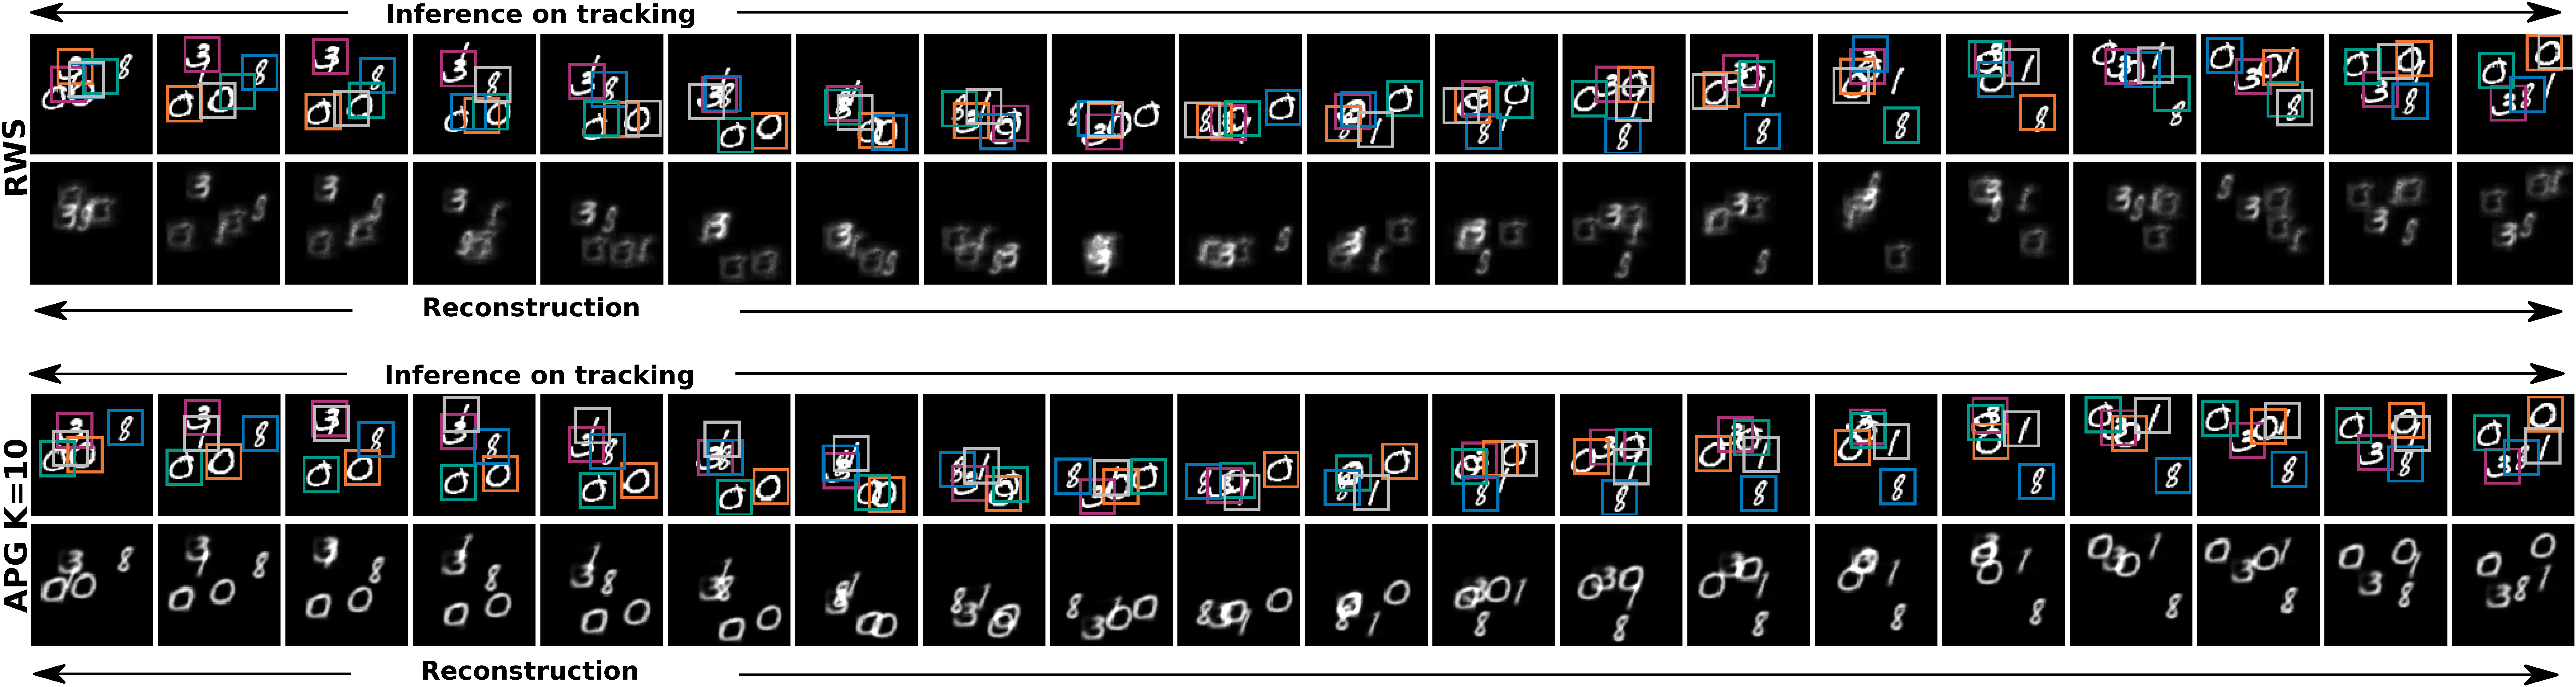
\includegraphics[width=150mm]{figures/bmnist-5digits-samples-with-rws-2.pdf}
\caption{Example 1.}
\end{figure*}

\begin{figure*}[th!]
\centering
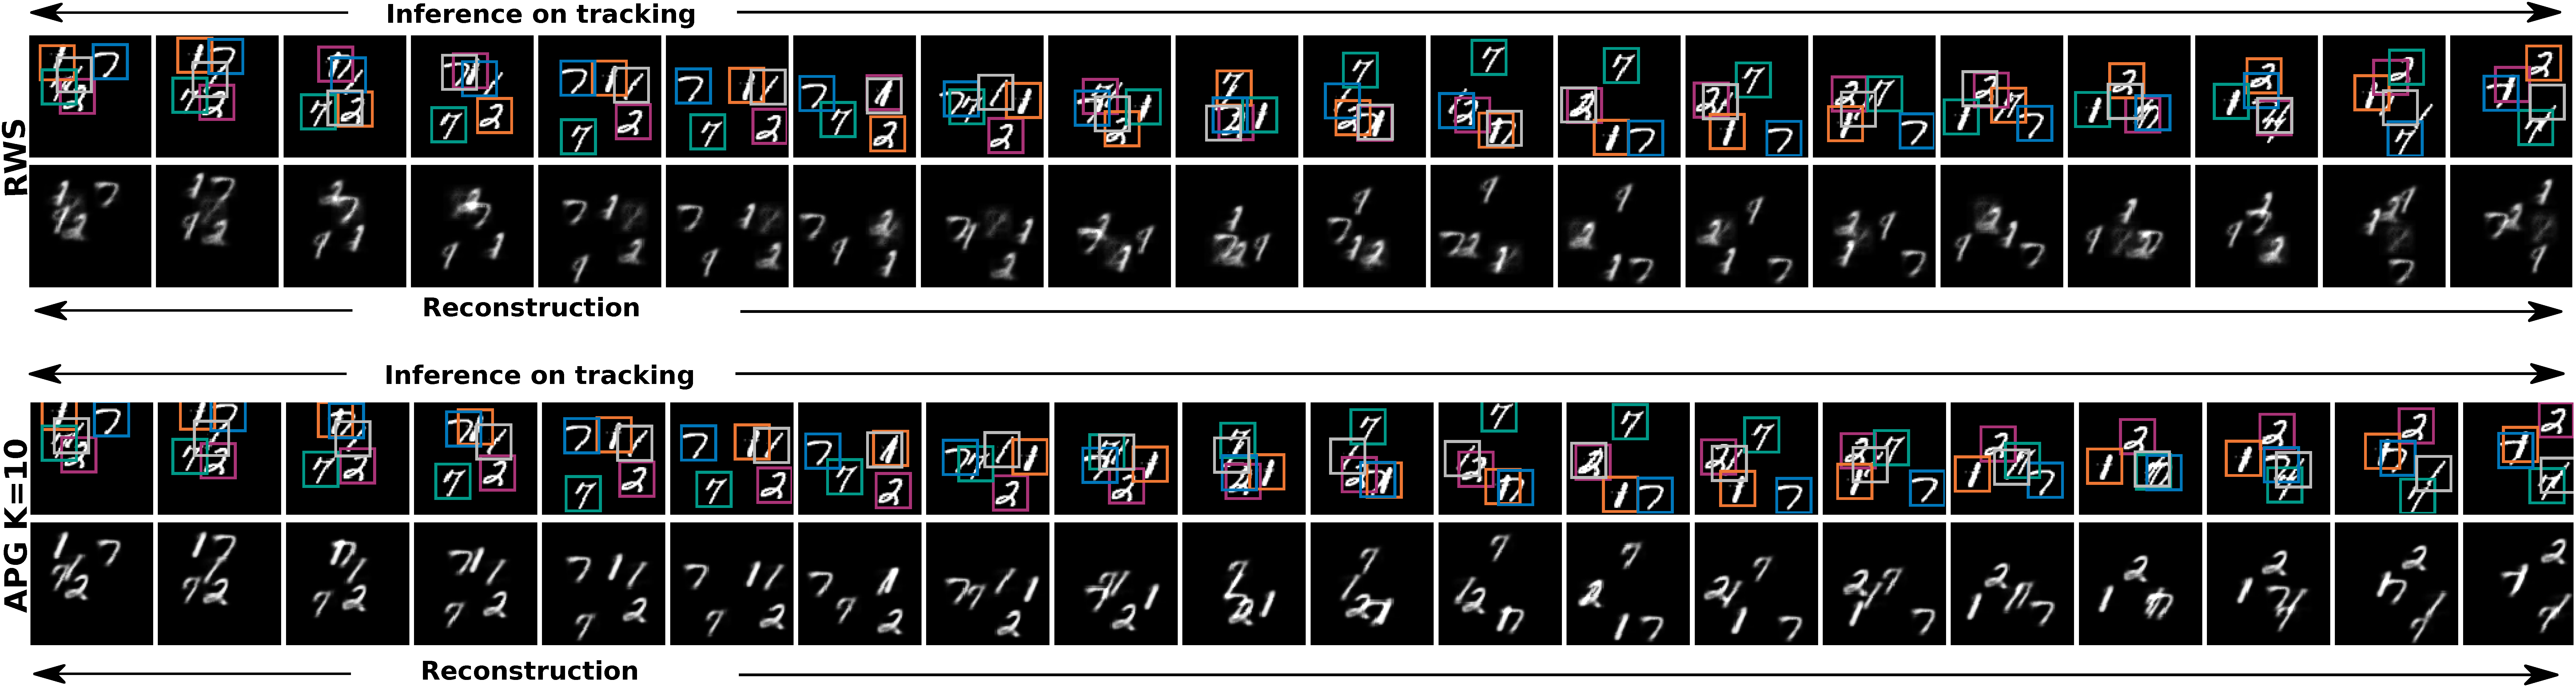
\includegraphics[width=150mm]{figures/bmnist-5digits-samples-with-rws-3.pdf}
\caption{Example 2.}
\end{figure*}

\begin{figure*}[h!]
\centering
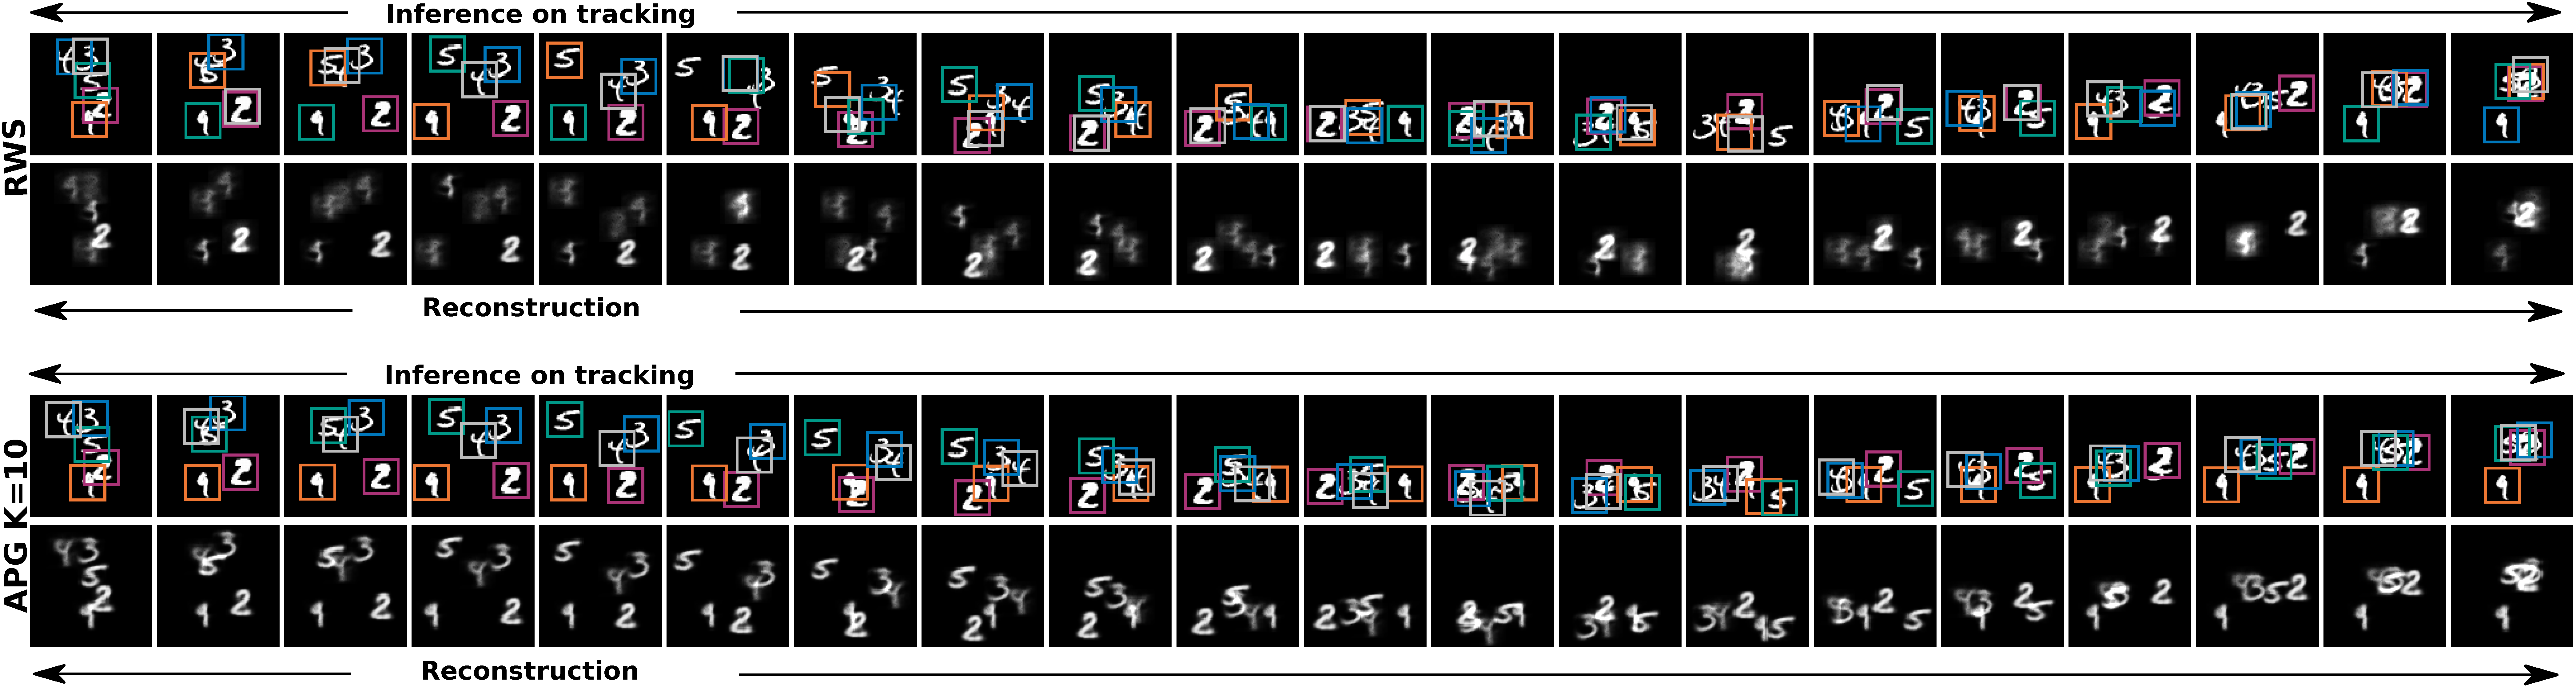
\includegraphics[width=150mm]{figures/bmnist-5digits-samples-with-rws-4.pdf}
\caption{Example 3.}
\end{figure*}


\newpage
\section{Inference Results and Reconstruction on large time steps Bouncing MNIST}
\label{appendix:full-recons}
The following are full reconstructions on test sets where time steps $T=100$ and number of digits $D=3, 4, 5$, respectively. In each figure, the 1st, 3rd, 5th, 7th, 9th rows show the inference results, while the other rows show the reconstruction of the series above.
\begin{figure*}[h!]
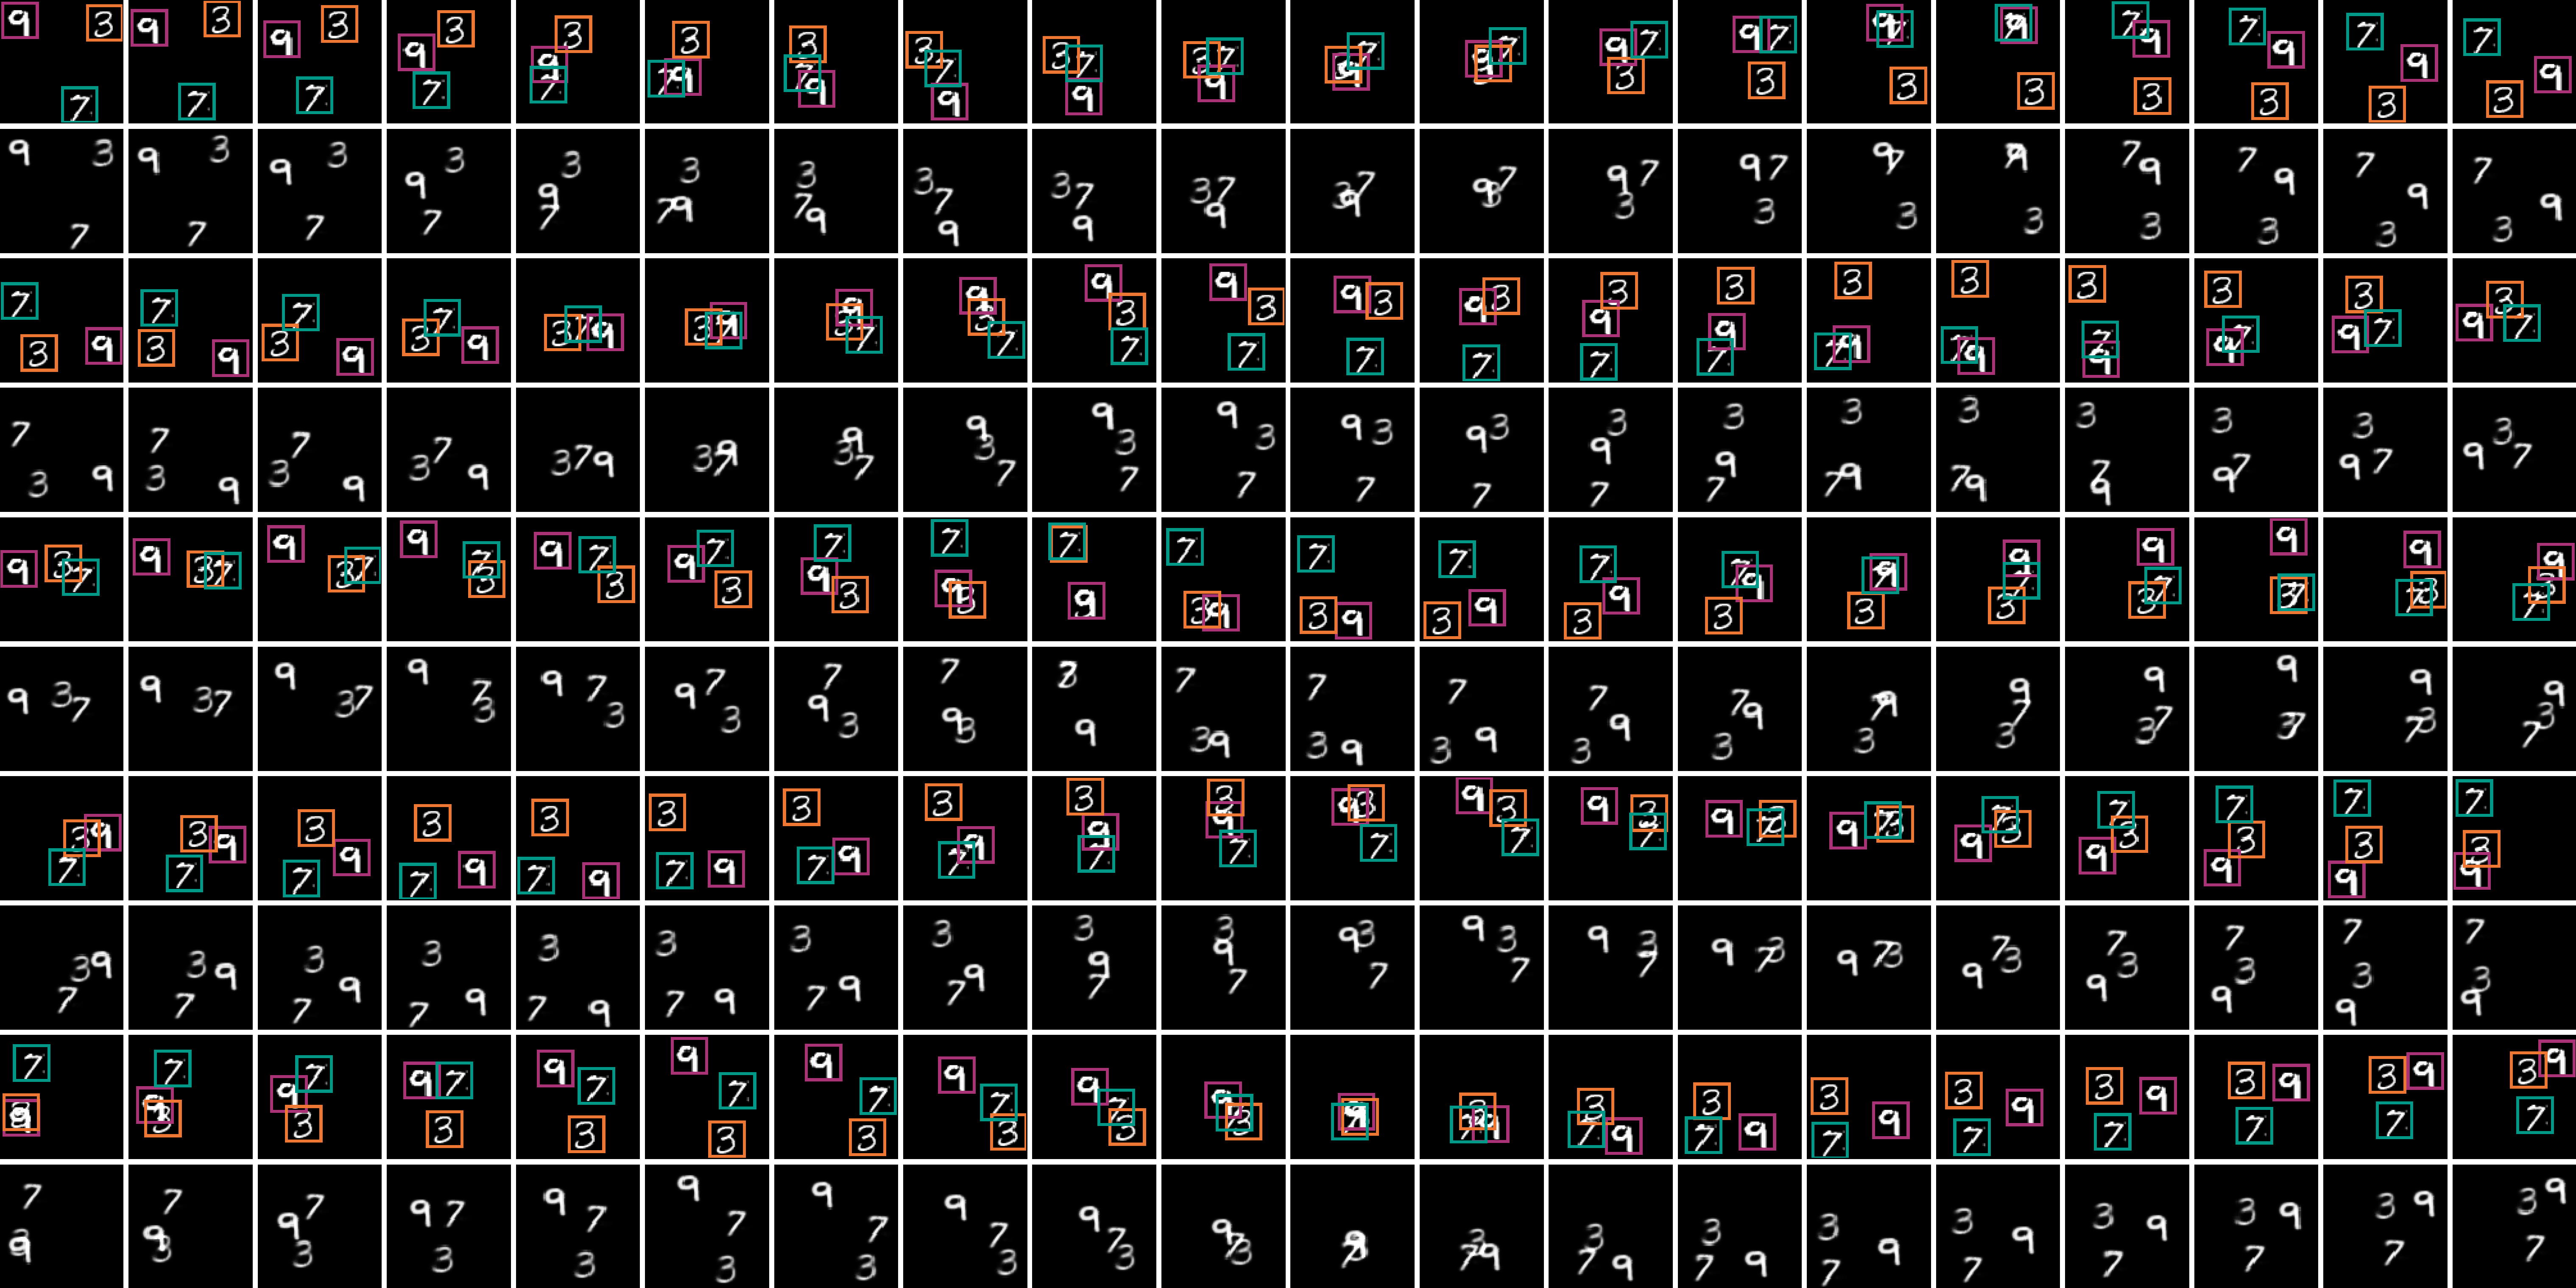
\includegraphics[width=170mm]{figures/T=100-D=3.pdf}
\caption{Full reconstruction for a video where $T=100, D=3$.}
\end{figure*}


\begin{figure*}[h!]
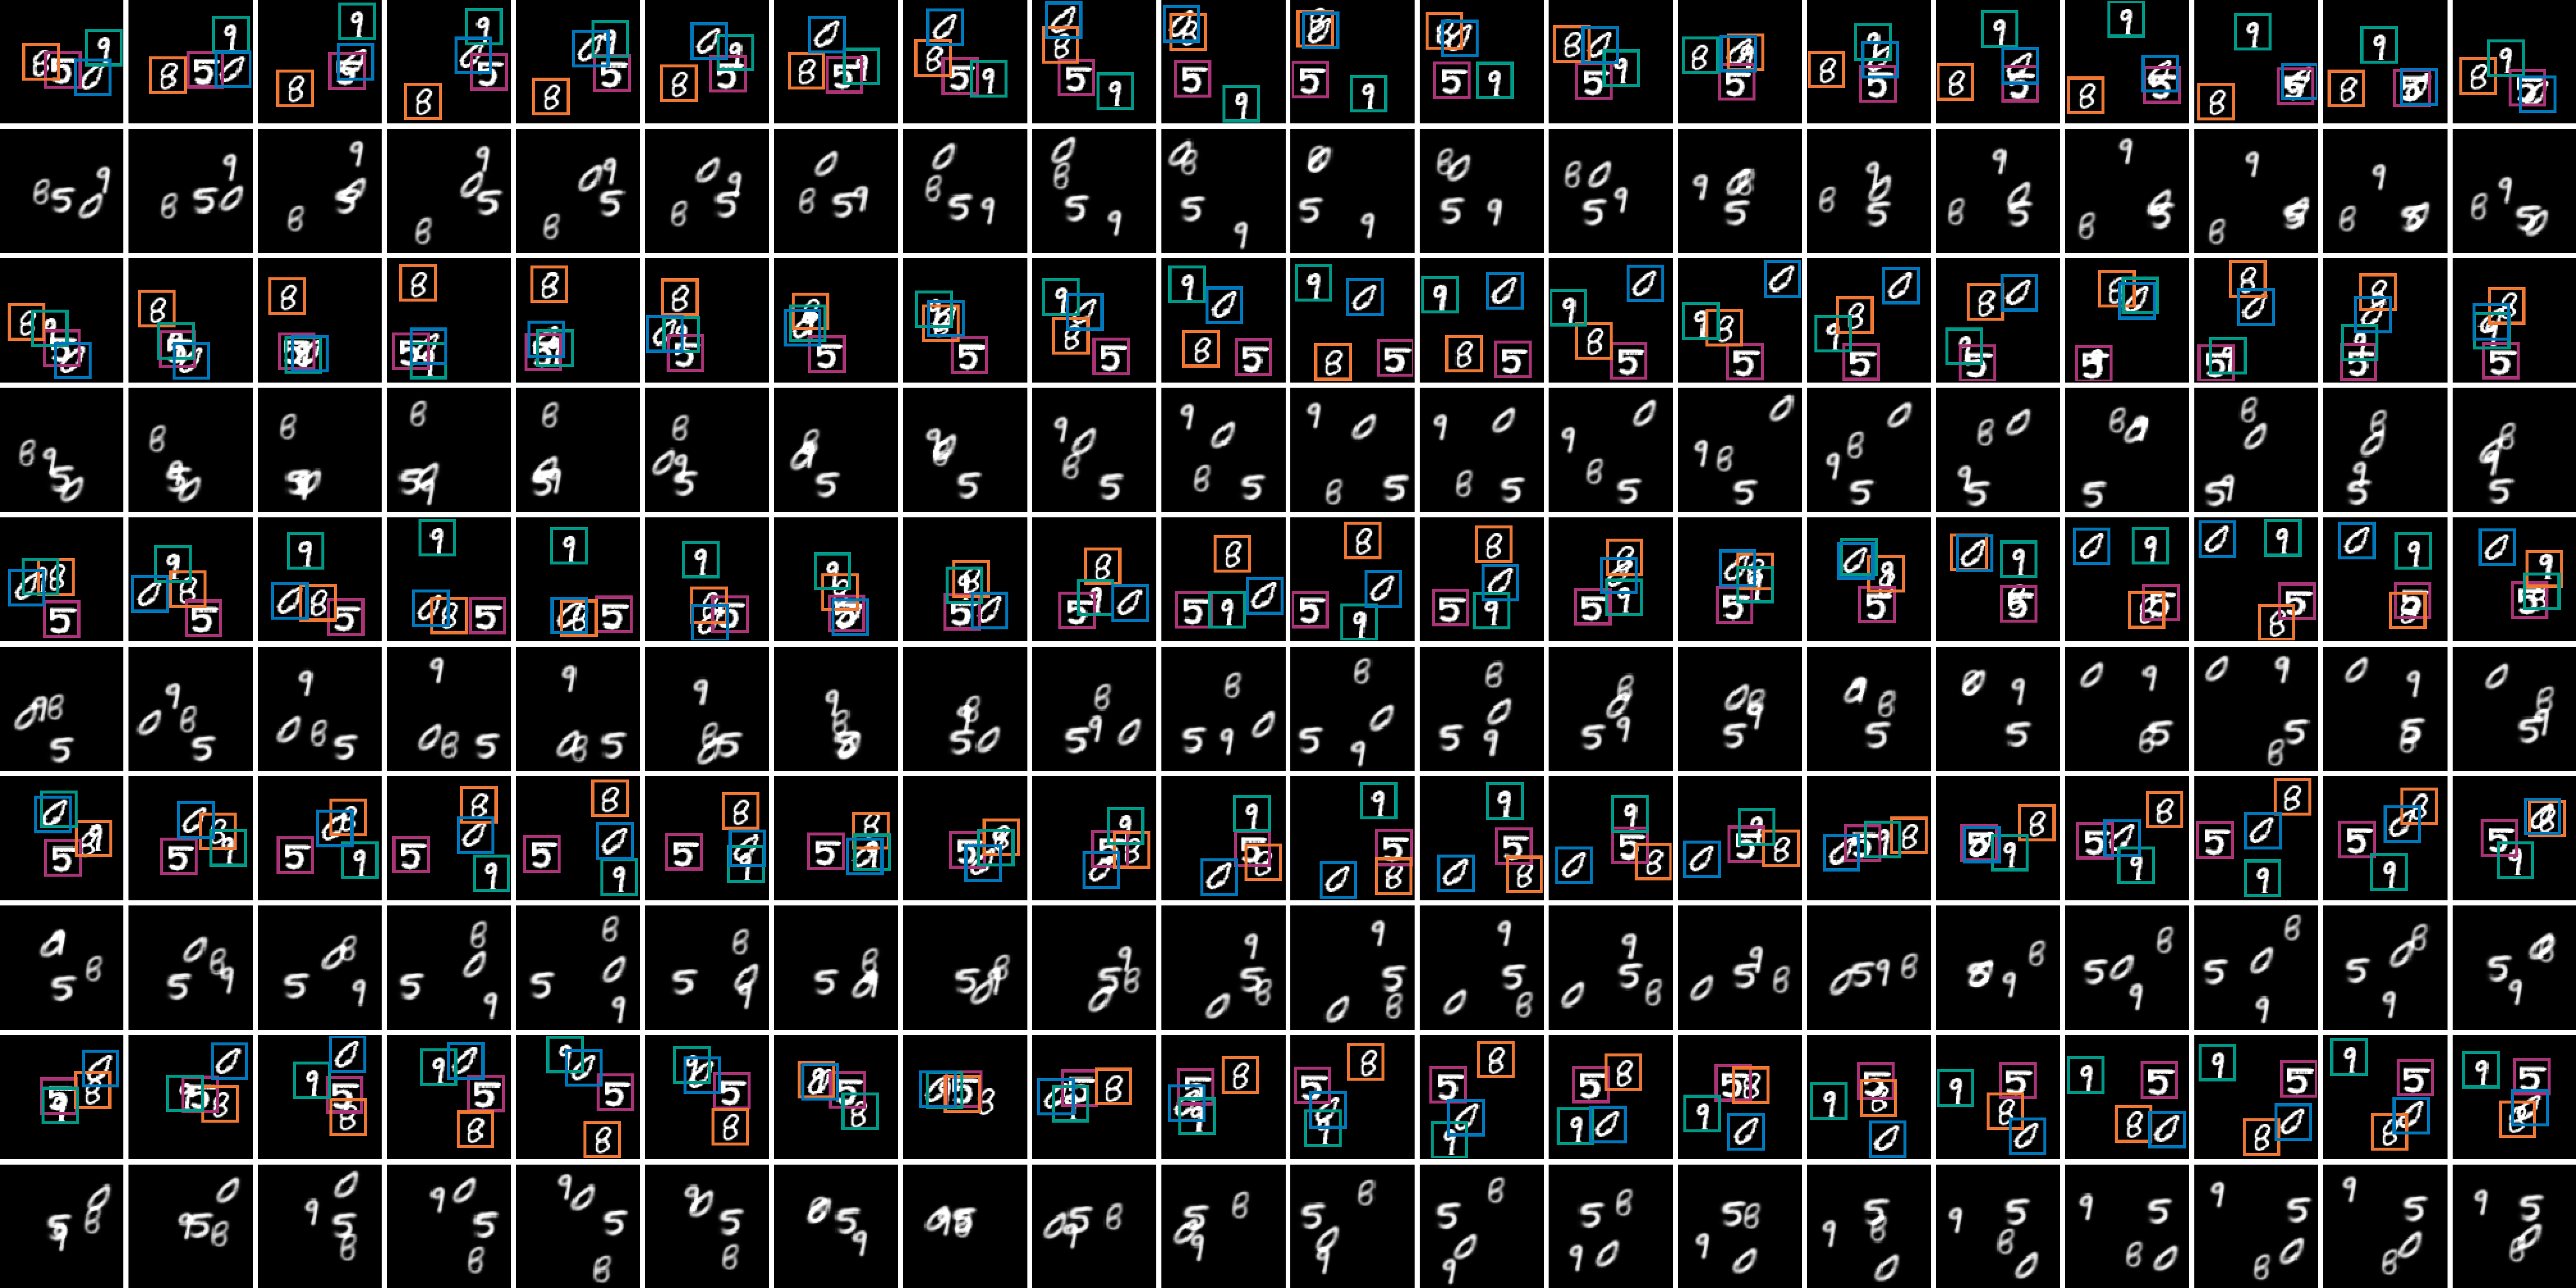
\includegraphics[width=170mm]{figures/T=100-D=4.pdf}
\caption{Full reconstruction for a video where $T=100, D=4$.}
\end{figure*}
\newpage
\begin{figure*}[h!]
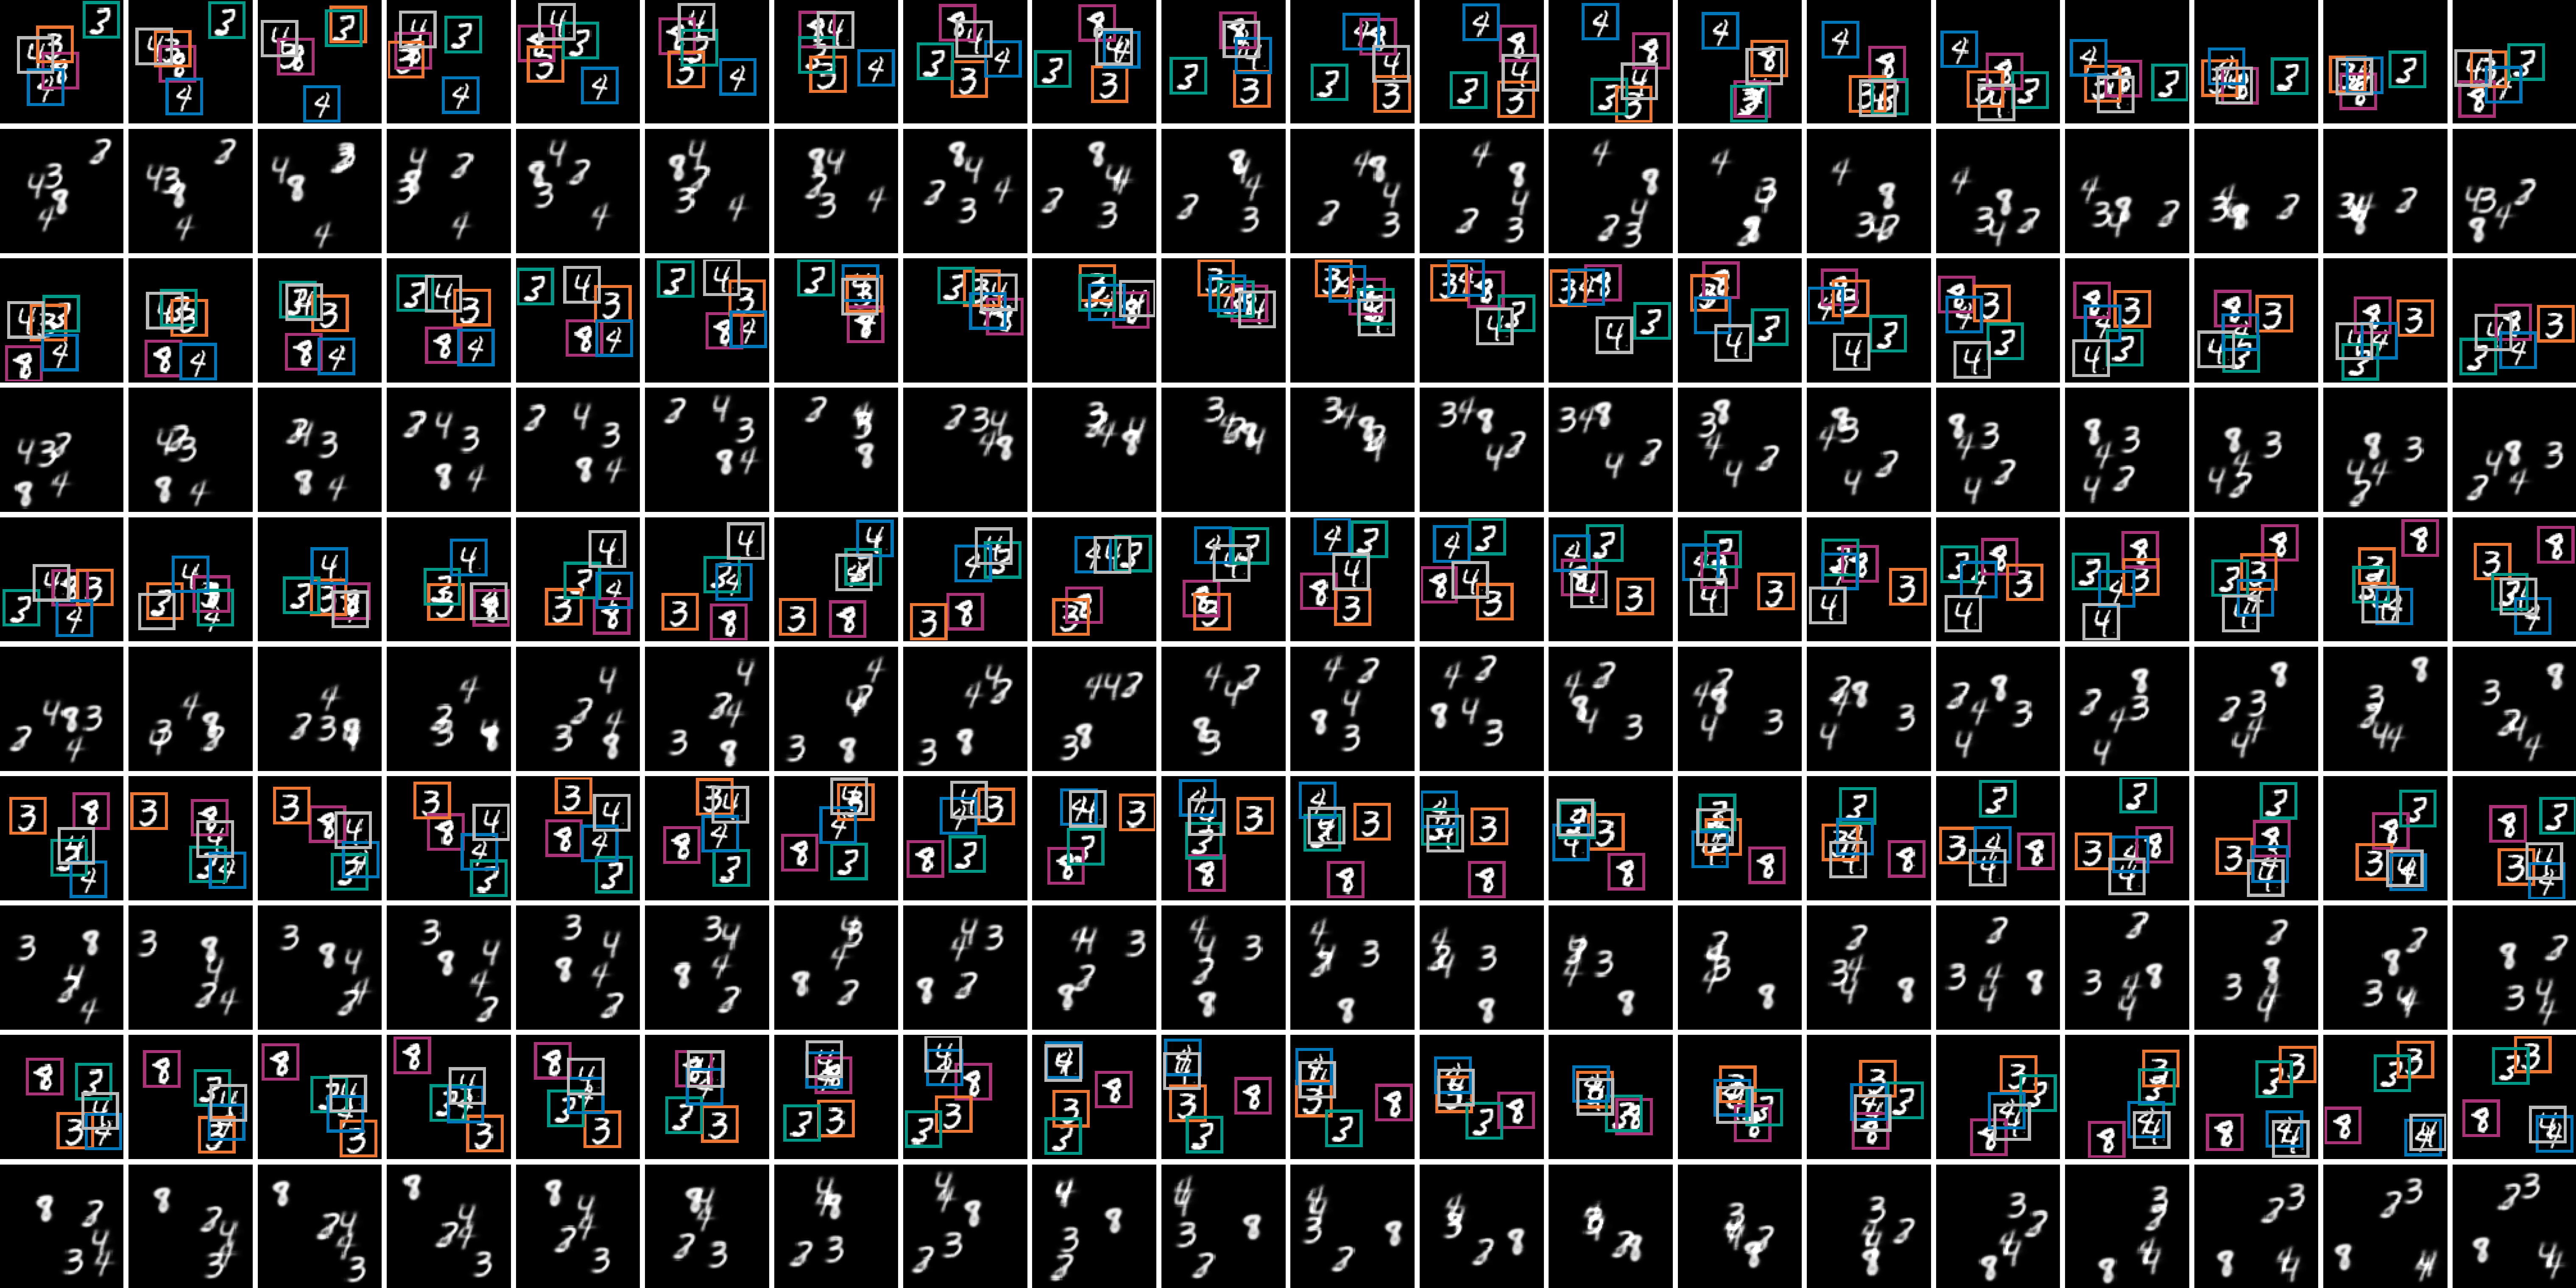
\includegraphics[width=170mm]{figures/T=100-D=5.pdf}
\caption{Full reconstruction for a video where $T=100, D=5$.}
\end{figure*}

\begin{figure*}[h!]
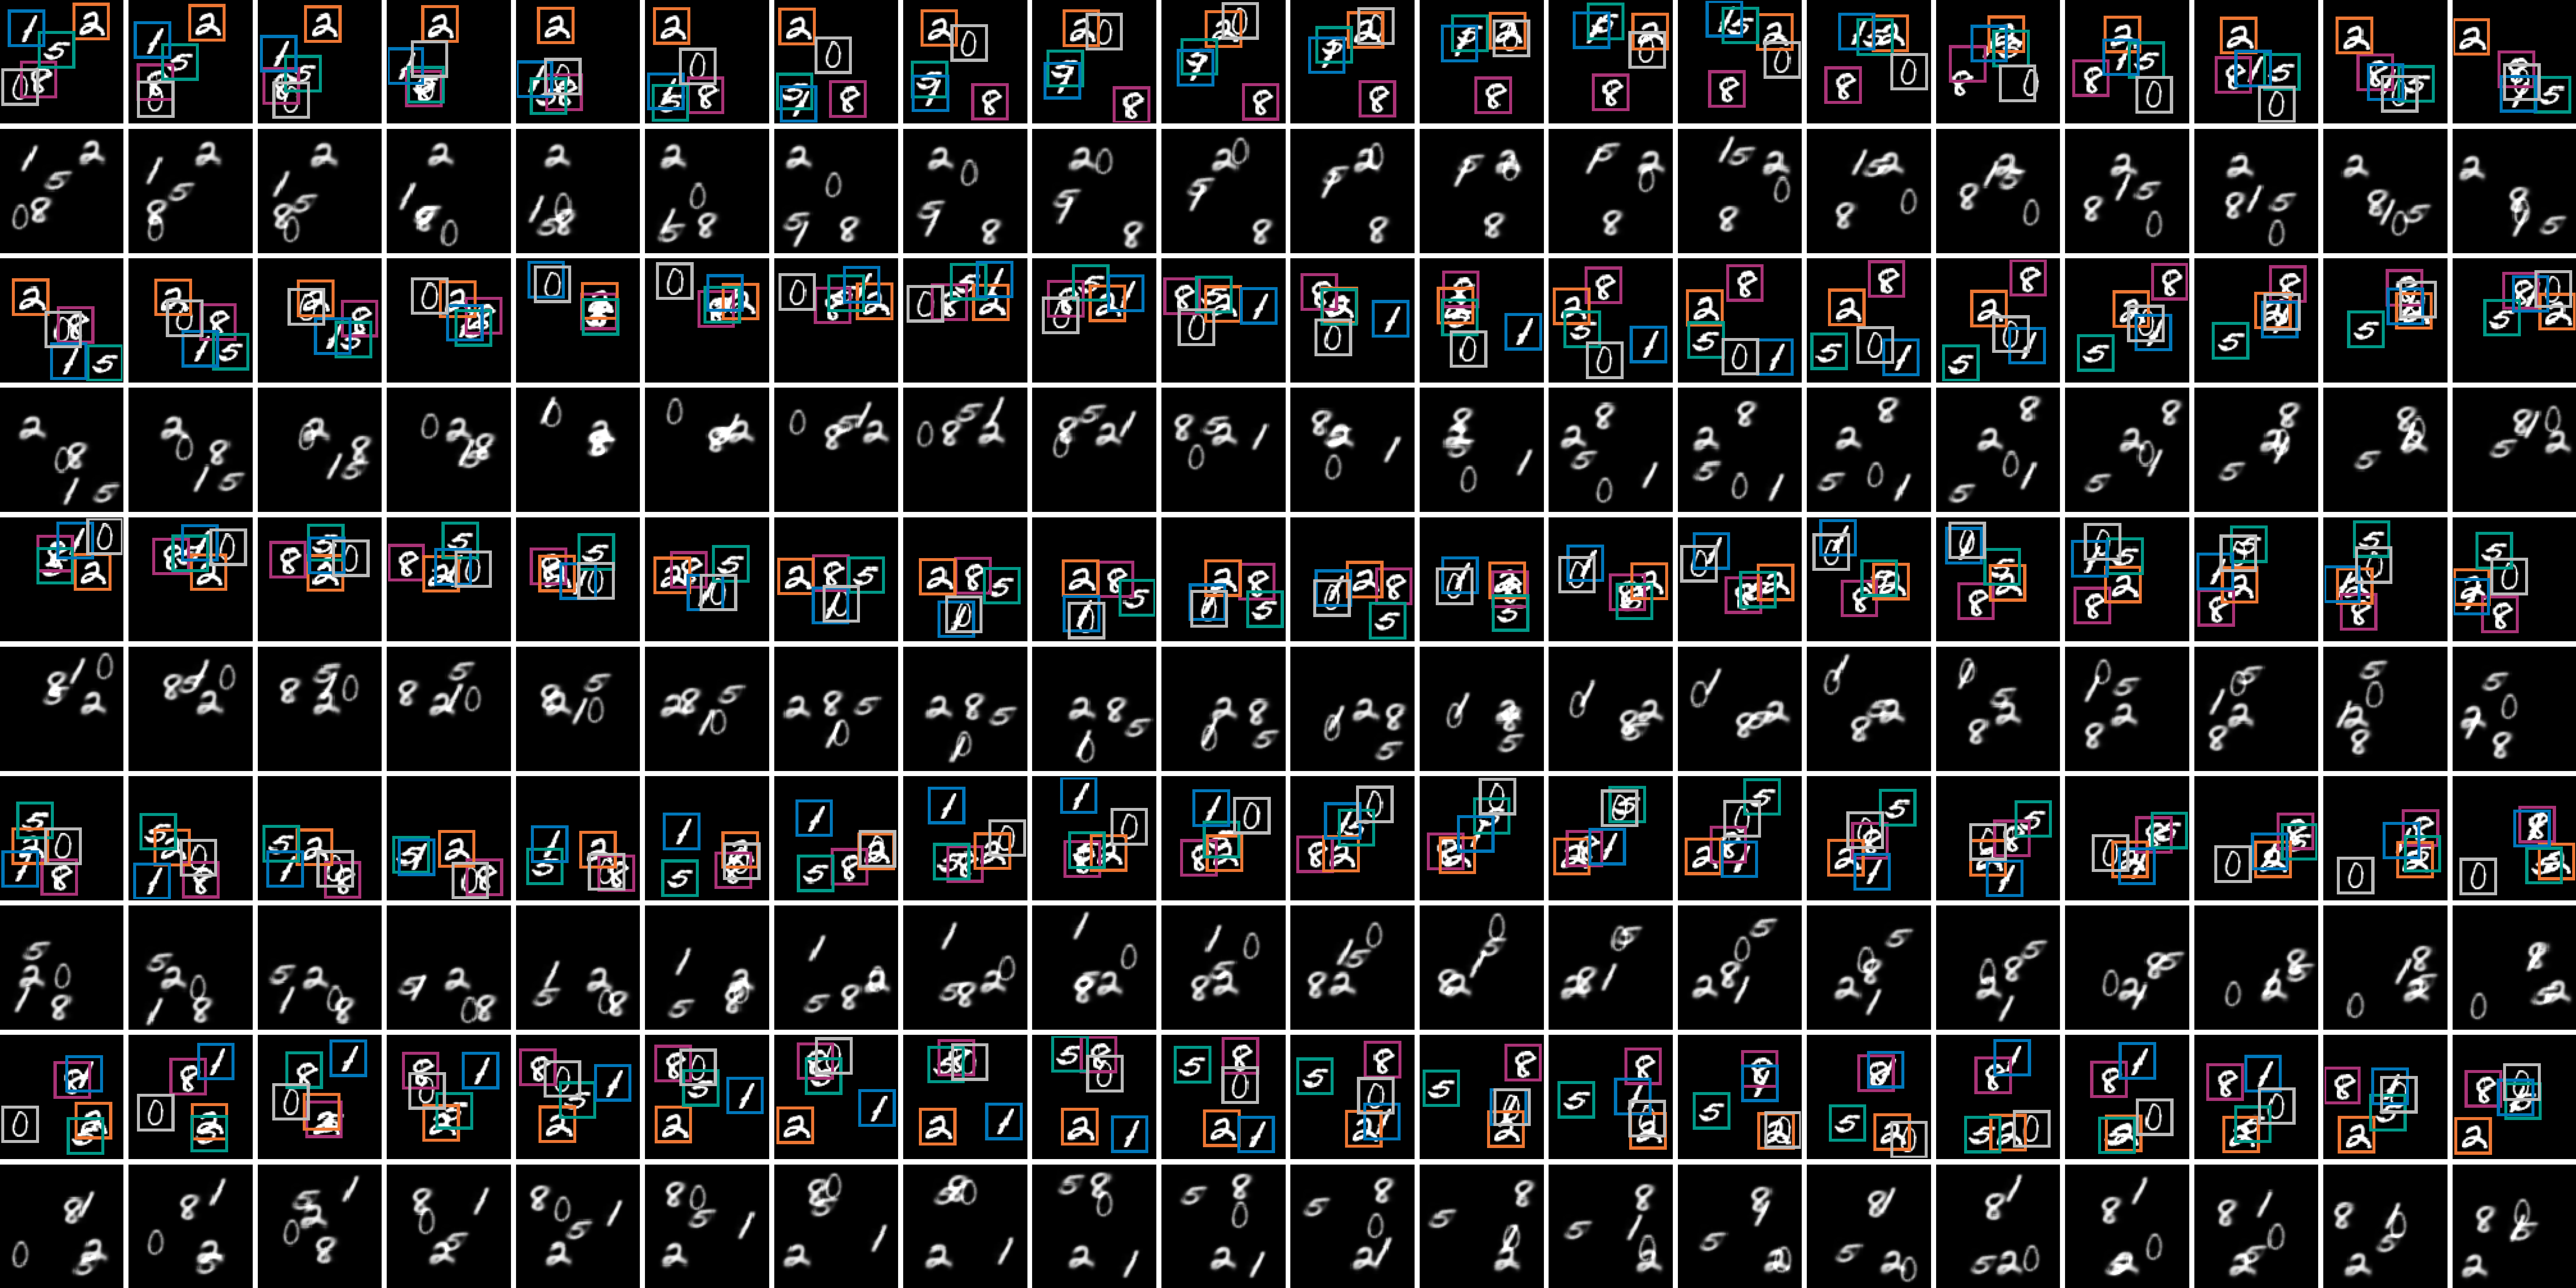
\includegraphics[width=170mm]{figures/T=100-D=5-2.pdf}
\caption{Full reconstruction for a video where $T=100, D=5$.}
\end{figure*}

% \appendix
% \section{Do \emph{not} have an appendix here}

% \textbf{\emph{Do not put content after the references.}}
%
% Put anything that you might normally include after the references in a separate
% supplementary file.

% We recommend that you build supplementary material in a separate document.
% If you must create one PDF and cut it up, please be careful to use a tool that
% doesn't alter the margins, and that doesn't aggressively rewrite the PDF file.
% pdftk usually works fine. 

% \textbf{Please do not use Apple's preview to cut off supplementary material.} In
% previous years it has altered margins, and created headaches at the camera-ready
% stage. 
%%%%%%%%%%%%%%%%%%%%%%%%%%%%%%%%%%%%%%%%%%%%%%%%%%%%%%%%%%%%%%%%%%%%%%%%%%%%%%%
%%%%%%%%%%%%%%%%%%%%%%%%%%%%%%%%%%%%%%%%%%%%%%%%%%%%%%%%%%%%%%%%%%%%%%%%%%%%%%%


\end{document}
